%%%  Pacchetto di stile A4  %%%
\documentclass[12pt,a4paper,oneside]{book}
\usepackage[T1]{fontenc} 
\usepackage[utf8]{inputenc}
\usepackage{phdthesis} % Pacchetto di stile per le tesi

% Ridefiniamo la riga di testa delle pagine:
\usepackage{fancyhdr}
\pagestyle{fancy}
\usepackage{titlesec}
\usepackage{setspace}
\usepackage{wrapfig}
\usepackage{sectsty}
\usepackage{adjustbox}
\usepackage{lipsum}
\usepackage{multicol}
\usepackage[font=footnotesize]{caption}
\usepackage{listings} %Per inserire codice
\usepackage[usenames]{color} %Per permettere la colorazione dei caratteri 
\definecolor{dkgreen}{rgb}{0,0.6,0}
\definecolor{gray}{rgb}{0.5,0.5,0.5}
\definecolor{mauve}{rgb}{0.58,0,0.82}

\definecolor{lightgray}{rgb}{.9,.9,.9}
\definecolor{darkgray}{rgb}{.4,.4,.4}
\definecolor{purple}{rgb}{0.65, 0.12, 0.82}
\renewcommand\lstlistingname{}
\lstdefinelanguage{javascript}{
  keywords={typeof, new, true, false, catch, function, return, null, catch, switch, var, if, in, while, do, else, case, break, for},
  keywordstyle=\color{blue}\bfseries,
  ndkeywords={class, export, boolean, throw, implements, import, this},
  ndkeywordstyle=\color{darkgray}\bfseries,
  identifierstyle=\color{black},
  sensitive=false,
  comment=[l]{//},
  morecomment=[s]{/*}{*/},
  commentstyle=\color{purple}\ttfamily,
  stringstyle=\color{red}\ttfamily,
  morestring=[b]',
  morestring=[b]"
}

\lstset{frame=tb,
  captionpos=b,
  abovecaptionskip=0.5cm,
  aboveskip=0.8cm,
  belowskip=0.3cm,
  showstringspaces=false,
  columns=flexible,
  basicstyle={\small\ttfamily},
  numbers=left,
  numberstyle=\tiny\color{gray},
  keywordstyle=\color{blue},
  commentstyle=\color{dkgreen},
  stringstyle=\color{red},
  breaklines=true,
  breakatwhitespace=true
  tabsize=4,
  frame=lrbt,
  rulecolor=\color{gray}
}
\renewcommand{\chaptermark}[1]{\markboth{#1}{}}
\renewcommand{\sectionmark}[1]{\markright{\thesection\ #1}}
\fancyhf{}
\fancyhead[RO]{\thepage}
\fancyhead[LO]{\leftmark}
\renewcommand{\headrulewidth}{0.1pt}
\renewcommand{\footrulewidth}{0pt}
\headsep=20pt
\sectionfont{\Large} 
\subsectionfont{\itshape\large} 
\titleformat{\chapter}[display]
  {\normalfont\huge\bfseries}{\chaptertitlename\ \thechapter}{20pt}{\huge}
\titlespacing*{\chapter}{0pt}{-10pt}{40pt}

\setlength{\skip\footins}{1cm}
\setlength{\footnotesep}{0.4cm}

\graphicspath{{./figure/}}	% path directory figure
\linespread{1.5}	% interlinea
%%%%%%

\usepackage{graphics,graphicx}

\usepackage{amsmath,amsfonts,amssymb,amsthm} % pacchetti tipici per scrivere matematica  
\usepackage{latexsym}
\usepackage{array}
\usepackage{tocbibind}
\usepackage{listings}  % listati di codice

\usepackage{cite}
\usepackage{algorithm}
\usepackage{algpseudocode}

\makeatletter
\def\BState{\State\hskip-\ALG@thistlm}
\makeatother

\usepackage{color}

\usepackage{textcomp}
\usepackage{subfigure}
\usepackage{subfloat}

% TOC INFO: sono le info salvate nelle proprieta' del file pdf
\hypersetup{ 
  pdftitle=Master Thesis in Computer Science,
  pdfauthor=Lorenzo Cioni,
  pdfsubject=Illuminant map analysis for image splicing detection
}    

%%%  Frontespizio  %%%

\university{}	% Universita' degli Studi di xxx (Firenze)
\faculty{Scuola di Ingegneria} %Nome della Scuola
\degree{}
\dept{} % nome dipartimento
\course{Corso di Laurea Magistrale in Ingegneria Informatica} %Corso di Laurea

\accademicyear{Anno Accademico 2015/2016} %anno accademico
\supervisor{Prof. Alessandro Piva} % relatore
\supervisor{Prof. Carlo Colombo} %correlatore
\advisor{Dott. Massimo Iuliani} %correlatore
\advisor{Dott. Marco Fanfani} %correlatore
\author{Lorenzo Cioni}

%titolo in italiano
%\title{\textbf{{\Huge Analisi della sorgente luminosa per la rivelazione di fotomontaggi}}}

%titolo in inglese
%\englishtitle{\textbf{{\Huge Illuminant map analysis for image splicing detection}}}
\title{\textbf{{\Huge Illuminant map analysis for image splicing detection}}}

\setcounter{tocdepth}{3}
\setcounter{secnumdepth}{3}

%%%  BEGIN DOCUMENT  %%%
\begin{document}

%%%  FRONT MATTER  %%%
\frontmatter
\maketitle  	% stampa la pagina di frontespizio

\chapter*{Abstract}
\addcontentsline{toc}{chapter}{Abstract}
\chaptermark{Abstract}

With the advent of powerful image editing tools, manipulating images and changing their content is becoming a trivial task. Unfortunately, most of the times, these modifications are aimed at deceiving viewers, changing their opinions or even affecting how people perceive reality. Therefore, the development of efficient and effective forgery detection techniques has become a hot research topic. 

From all types of image forgeries, image compositions are specially interesting. This type of forgery uses parts of two or more images to construct a \emph{new reality} from scenes that never happened. Among all different telltales investigated for detecting image compositions, illumination inconsistencies are considered the most promising ones since a perfect light matching in a forged image is still difficult to achieve. 

This thesis builds upon the hypothesis that image illumination inconsistencies are strong and powerful evidence of image composition and presents an extension of two approaches in literature, both based on the illuminant maps analysis. The first method is specific for human face forgeries, the second is a blind approach for detecting regional splicing.


\chapter*{Sommario}
\addcontentsline{toc}{chapter}{Sommario}
\chaptermark{Sommario}

Con l'avvento di sempre più potenti strumenti di modifica di immagini, la manipolazione di contenuti visuali è diventata un'operazione molto comune. Purtroppo, il più delle volte, queste modifiche sono volte ad ingannare gli spettatori, cambiare le loro opinioni o perfino a modificare il modo in cui percepiscono la realtà. Di conseguenza, lo sviluppo di tecniche sempre più efficienti ed efficaci per la rilevazione di fotomontaggi  è diventato un argomento di ricerca molto importante. 


Tra tutti i tipi di falsificazione, la composizione di più immagini è particolarmente interessante. Questo tipo di operazione utilizza le parti di due o più immagini al fine di costruire una vera e propria nuova realtà, ricostruendo scene mai accadute realmente. Tra tutte le diverse tecniche di rilevazione di composizione di immagini, quelle basate sulle inconsistenze della luce sono considerate fra le più promettenti, poiché è quasi sempre difficile riuscire a rispettare la coerenza di illuminazione all'interno della stessa immagine quando questa viene modificata.

Questa tesi pone le sue basi proprio sull'ipotesi che l'individuazione di inconsistenze nella luce presenti in un'immagine sia una prova evidente di contraffazione. A partire da questa ipotesi, è presentata un'analisi ed un'estensione di due approcci presenti in letteratura che pongono le loro basi sulle \emph{Illuminant Maps}. Il primo metodo è specifico per la rilevazione di contraffazioni che riguardano volti umani nelle immagini; il secondo invece è un approccio molto più generico che cerca di individuare zone dell'immagine che presentano delle inconsistenze nel colore dell'illuminante.

% DEDICA
\newpage{\thispagestyle{empty}\null\vfil
\begin{flushright}
\textit{{\large Dedica}}
\end{flushright}
}


\tableofcontents

%% Corpo della tesi

\mainmatter{
\chapter*{Introduction}
\addcontentsline{toc}{chapter}{Introduction}
\chaptermark{Introduction}

With the rapid development of multimedia and network technology, digital images, as an effective carrier of information, are having a more and more important impact on people's daily lives. 

However, the image content can easily be tampered with the increasingly powerful image processing software, which threatens the integrity and authenticity of digital images. Moreover, if the tampered images were used for illegal purposes, there would be no doubt causing extremely bad effects on both the individual and society.

Images manipulated with the purpose of manipulating and deceiving user opinions are present in almost all communication channels including newspapers, magazines, TV shows and, obviously, on Internet.\cite{rocha2011vision}

Image splicing is a fundamental operation used in digital image tampering. It is a copy-and-paste
operation of image regions from one image onto the same or another image without performing post-processing such as smoothing \cite{ng2004blind}. Even without post-processing, the artifacts introduced by
image splicing may be almost imperceptible. Therefore, the detection of image splicing is a preliminary but desirable study for image forensics.

Generally speaking, there are two approaches of image forgery detection: active and passive detection. 

Active approaches require pre-processing (e.g. watermark embedding  \cite{rey2002survey}\cite{ye2005watermarking}) when generating the image and a post-processing on image distribution.

Passive approaches \cite{ng2006passive} do not need this operation and could make analysis on various images based on supervised learning. Hence, it gains more attention and becomes
a hot research topic in image forensics.

Investigating image's lighting is one of the most common approaches for splicing detection. This kind of approach is particularly robust since it's really hard to preserve the consistency of the lighting environment while creating an image composite (i.e. a splicing forgery). 

In this scenario, there are mainly two main approaches:
\begin{enumerate}
\item based on the object-light geometric arrangement
\item based on the image illuminant colors
\end{enumerate}

We focused our attention on the illuminant-based approach, which assumes that a scene is lit by the same light source. More light sources are admitted but far enough such as to produce a constant brightness across the image. In this condition, pristine images will show a coherent illuminant representation; on the other hand, inconsistencies among illuminant maps will be exploited for splicing detection. 

\emph{Illuminant maps} locally describes the lighting in a small region of the image. In the computer vision literature exists many different approaches for determining the illuminant of an image. In particular, such techniques are divided into two main groups: statistical-based and physics-based approaches.

Regarding the first group, we start investigating on the \emph{Grey-World algorithm} \cite{Buchsbaum19801}, which is based on the Grey-World assumption, i.e. the average reflectance in a scene is achromatic. In \cite{finlayson2004shades}, this algorithm proved to be special instances of the Minkowski-norm. Van de Weijer et al. \cite{van2007edge} than proposed an extension of the Gray-World assumption, called \emph{Gray-Edge hypothesis} \cite{van2007edge}, which assumes that the average of the reflectance differences in a scene is achromatic. 

These differences can be determined by taking derivatives of the image. Therefore, the authors present a framework with which many different algorithms can be constructed.
We focus our attention on this framework, called \emph{Generalized Grey-World algorithm} (GGE).

For the latter group, was investigate the method proposed by Riess et al. \cite{riess2010scene}, which extends the \emph{Inverse Intense Chromaticity} (\emph{IIC}) space approach proposed by Tan et al. \cite{tan2004color} and tries to model the illuminants considering the dichromatic reflection model \cite{tominaga1989standard}. In this case, the illuminant map is evaluated dividing  images into blocks, named \emph{superpixels}, of approximately the same object color, then the illuminant color is evaluated for each block solving the lighting models locally. 

Carvalho et al. \cite{carvalho2016illuminant} then presents a method that relies on a combination of the two approaches for the detection of manipulations on images containing human faces. In addition to maps, a large set of shape and texture descriptors are used together. Note that, from a theoretical viewpoint, it is advantageous to consider only image regions that consist of approximately the same underlying material: for this reason, in \cite{carvalho2016illuminant} the authors focused their analysis on human faces.

This work is structured as follows. Chapter 2 describes the main methods grounded on illumination inconsistencies for detecting image composition and the background theories on which this work is based on. In Chapter 3 our contributions for detecting image splicing is presented. Finally, Chapter 4 collects the experimental results, putting our research in perspective and discussing new research opportunities.
\chapter{Related work}

\section{Image forgery}

When dealing with a digital image, it is quite common to wonder if it is original or it has been counterfeited in some way. Images and videos have become the main information carriers in the digital era and they are used to store real world events, but they are very easy to manipulate because of the availability of powerful editing softwares and sophisticated digital cameras.

The contexts where doctored pictures could be involved are very disparate; they could be used in a tabloid or in an advertising poster or included in a journalistic report but also in a court of law where digital (sometimes printed) images are presented as crucial evidences for a trial in order to influence the final judgement. 

Generally speaking, the objective of the image editing operation could be, for example, to improve its quality or to change its semantic content \cite{piva2013overview}. In the first case, the processed image will carry the same information as the original one, but in a more usable/pleasant way. Hence, we refer to this kind of editing as \emph{innocent}. In the latter case, the semantic information conveyed by the image is altered, usually by adding or hiding some information. This kind of editing is considered \emph{malicious} \cite{piva2013overview}.

Forgeries can be classified into three categories:

\begin{itemize}
\item \emph{Copy-move forgery}
\item \emph{Image retouching}
\item \emph{Image splicing}
\end{itemize}

\emph{Copy-move forgery} is one of the most popular forms of tampering in which some regions are copied from a particular location in an image and thereafter pasted at one or more locations within the same image or a different image of preferably the same scene. This technique is useful when the forger wants either to hide or duplicate something that is already present in the original image.

\emph{Image retouching} is an image editing method that pertains to a slight change in the image for various aesthetic and commercial purposes, not necessarily conforming to the standards of morality. The retouching is mostly used to enhance or reduce the image features. Usually this type of forgery is realised by changing the colour or texture of the objects, intensify the weather conditions or simply
introducing some blur for defusing the objects.

\emph{Image splicing}, also known as \emph{cut-and-past attack}, is another common form of photographic manipulation. This kind of forgery involves the composition of more than one image that are combined together to generate a tampered image, usually to alter its content and original meaning \cite{qazi2013survey}\cite{piva2013overview}. When performed carefully, the border between the spliced regions can be visually imperceptible. 

\begin{figure}
  \centering
    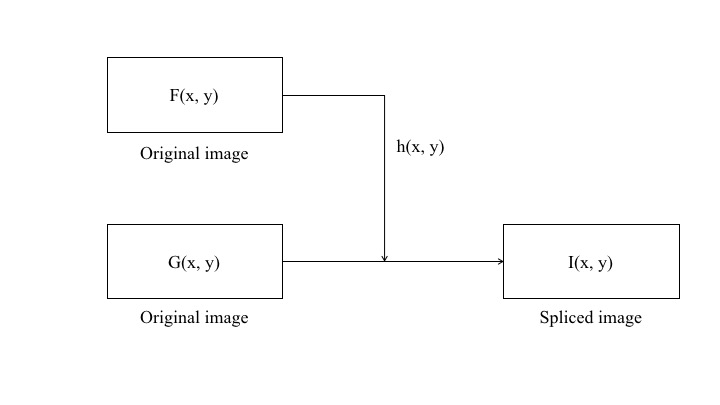
\includegraphics[width=0.8\textwidth]{imagesplicing}
    \caption{Image splicing process}
\end{figure}

This composition process includes all the necessary operations (such as brightness and contrast adjustment, affine transformations, color changes, etc.) to construct realistic images able to deceive viewer. In this process, normally, we refer to the parts coming from other images as \emph{aliens} and to the image receiving the other parts as \emph{host}. One common studied case is image composition involving very popular people, which can be employed with many different aims.

\subsection{Some famous cases}

Photography has lost its innocence since the early days of its birth. Image forgery can be traced back to as early as 1840s when Hippolyte Bayrad created the very first fake image \ref{fig:firsttampered}, in which he was shown committing a suicide, only a few decades after Niépce created the first photo.

\begin{figure}[!h]
  \begin{center}
    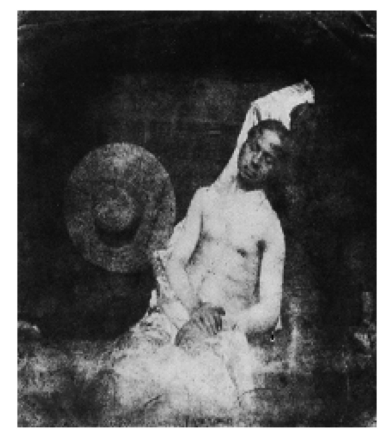
\includegraphics[width=0.35\textwidth]{firsttampered}
  \end{center}
  \caption{The first tampered image}\label{fig:firsttampered}
\end{figure}

\paragraph{O.J. Simpson - June 1994}

This altered photo of O.J. Simpson (Fig. \ref{fig:ojsimpson}) appeared on the magazine's cover Time Magazine, soon after his arrest for murder. 

\begin{figure}[!h]
  \begin{center}
    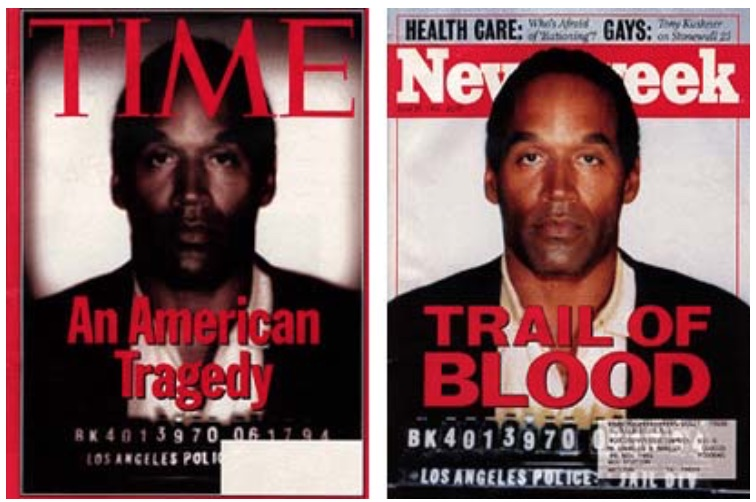
\includegraphics[width=0.45\textwidth]{ojsimpson}
  \end{center}
  \caption{The Time Magazine cover with O.J. Simpson}\label{fig:ojsimpson}
\end{figure}

In fact, the photograph was altered compared to the original image that appeared on the cover of Newsweek magazine. Time magazine was accused of manipulation of the photography in order to make darker and more menacing the figure of Simpson.

\paragraph{Iraq - April 2003}

This composition (Fig. \ref{fig:iraq}) of a British soldier in Basra, who keeps pointing toward a civilian Iraqi gesticulating, appeared on the cover of the Los Angeles Times, immediately after the Iraq invasion. 

Brian Walski, a staff photographer for the Los Angeles Times was summarily fired from his publisher because he merged two of his shots in order to improve the composition.

\begin{figure}[!h]
  \begin{center}
    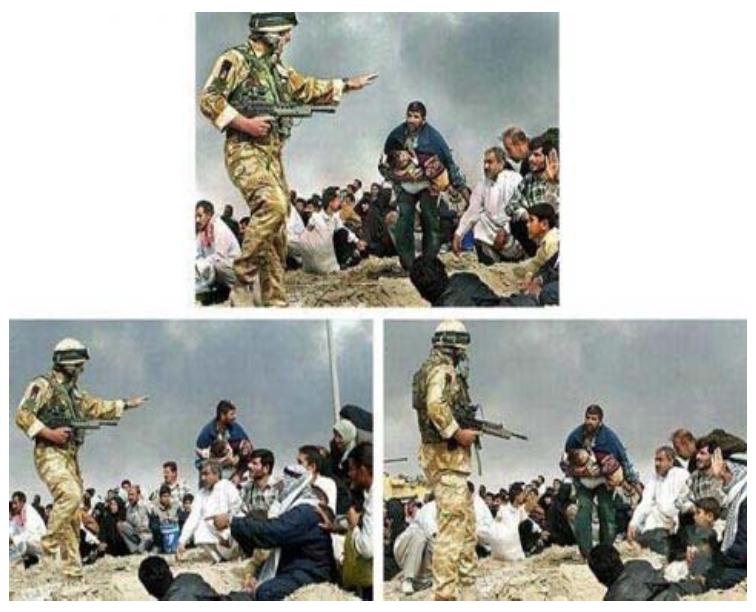
\includegraphics[width=0.60\textwidth]{iraq}
  \end{center}
  \caption{An example of image composition}\label{fig:iraq}
\end{figure}

\paragraph{George W. Bush - March 2004}

This image (Fig. \ref{fig:bush}), taken from the election campaign of George W. Bush, outlined a packed audience of soldiers as a backdrop to a child who was flying the American flag. This image was digitally edited, using a crude copy and paste, removing Bush from the podium. 

\begin{figure}[!h]
  \begin{center}
    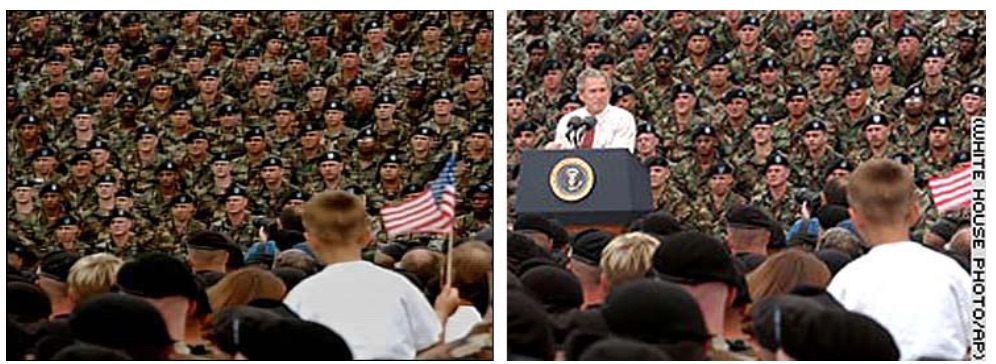
\includegraphics[width=0.60\textwidth]{bush}
  \end{center}
  \caption{An example of image composition}\label{fig:bush}
\end{figure}

Cases like these show how present image composition is in our daily lives. Unfortunately, it also decreases our trust on images and highlights the need for developing methods for recovering back such confidence.

\section{Image forgery detection techniques}

As a consequence of all previous facts, a reliable assessment of image integrity becomes of fundamental importance\cite{zhu2004seeing} \cite{farid2009digital} \cite{piva2013overview}.

Forgery detection intends to verify the authenticity of images.  The research community interested in multimedia content security has proposed several approaches aimed at detecting image forgeries that can be classified into \emph{active} and \emph{passive} techniques.

\begin{figure}[!h]
  \begin{center}
    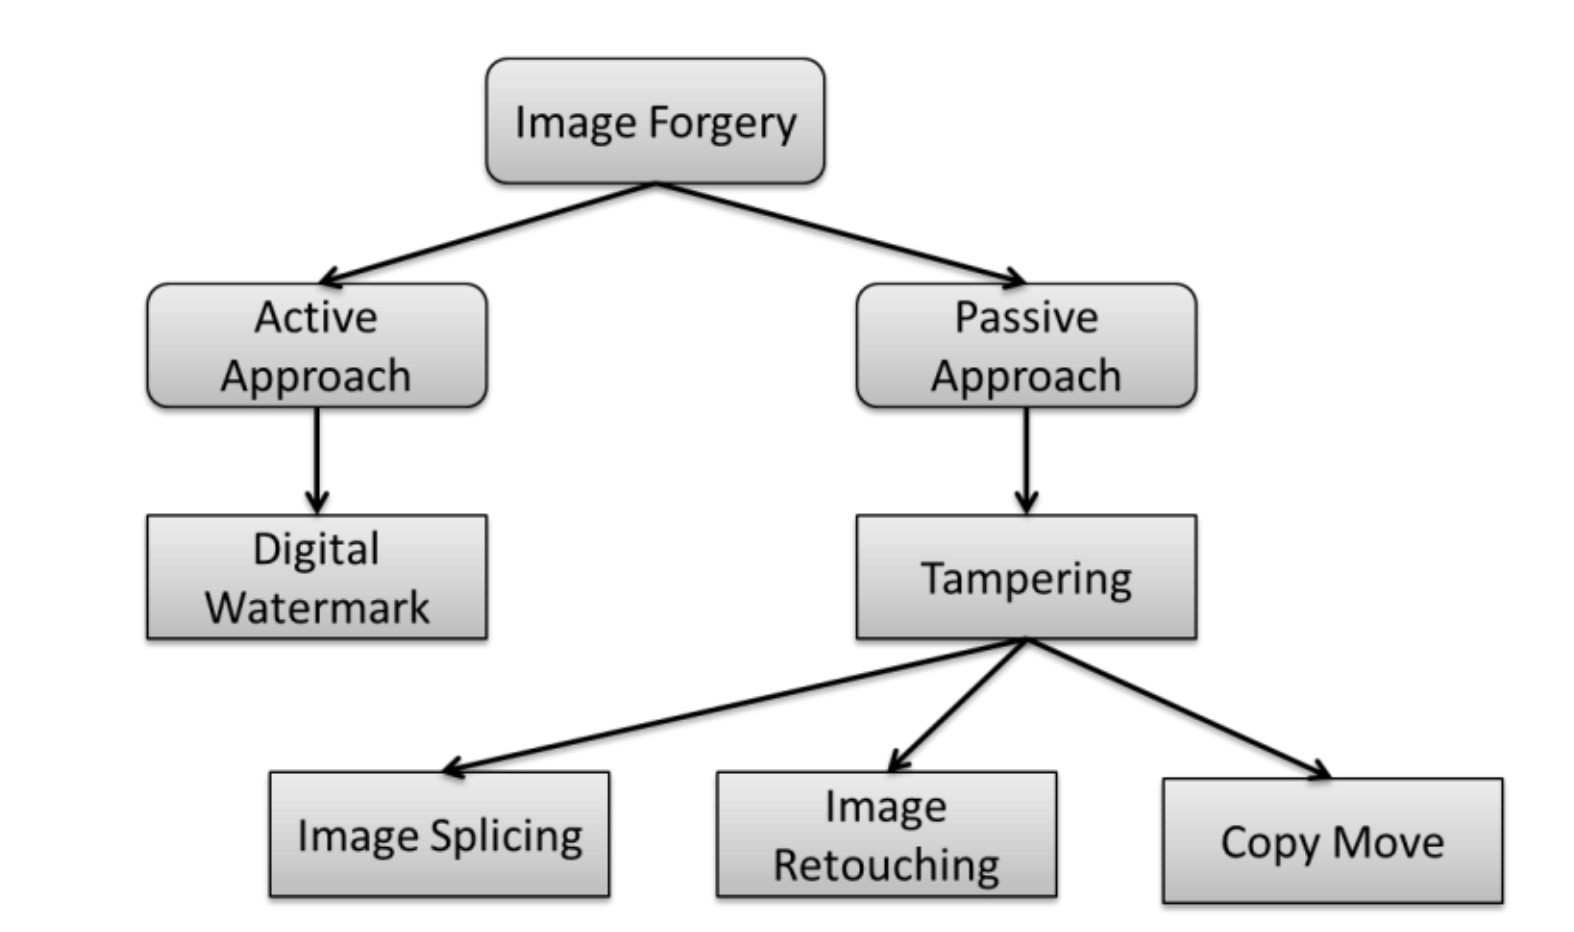
\includegraphics[width=0.75\textwidth]{forgerydetectionclass}
  \end{center}
  \caption{Image forgery detection approaches classification}
    \label{fig:forgerydetectionclass}
\end{figure}

\subsection{Active approaches}

Active approaches basically envolve the data hiding approaches and the digital signature approaches. Active approaches are inspired by the idea of granting authenticity to the images generated by digital cameras. \cite{friedman1993trustworthy} \cite{blythe2004secure}. 

In this kind of methods, some additional information is embedded into the image at the instant of its acquisition and any later modification can be detected by checking the value of the \emph{digital watermark} \cite{cox2002digital}\cite{katzenbeisser2000information}\cite{cox2007digital} or the \emph{digital signature}\cite{rivest1978method}\cite{pointcheval2000security}\cite{nikolaidis1996copyright} at the moment of its fruition. Therefore these techniques are also called intrusive techniques \cite{mahdian2010bibliography}. 

The major drawback of these schemes is that they must be used by the image capturing device itself at the time of recording or later by an authorized person, using a specialized embedding software. Therefore, specially equipped cameras or special hardware and software are needed. Furthermore, this kind of approaches may degrade the quality of the original image \cite{van2007survey}.

From the implementation point of view, active approaches need specially equipped camera consisting of a watermarking or a digital signature chip and some private key hard-wired in the camera itself, using which every image captured by the image is authenticated before saving it on its memory card. 

\subsection{Passive approaches}

Passive approaches\cite{ng2006passive} were proposed to overcome the problems encountered in the active approaches. These schemes do not require any image preprocessing and do not alter the image content.  

These approaches are based on the fact that the digital image has some consistent inherent
patterns (statistical properties) which are acquired from the distinct phases that are part of the image history \cite{piva2013overview}, like the acquisition phase, storage and compression, post processing operations etc.. Each phase leaves a unique trace on the image, which works as a digital fingerprint.
These patterns are altered during image forgery operations is performed on the image and the mutated image properties can be detected by applying some statistical image functions.

This technology, defined as \emph{multimedia forensics}\cite{farid2009image}\cite{van2007survey}\cite{mahdian2010bibliography}, deals with such issues by studying and developing technological tools which generally permit determining, by only analyzing a digital photograph, if the considered asset has been manipulated or even which could have been the adopted acquisition device. Moreover, if it has been determined that something has been altered, it could be important to understand in which part of the image itself such modification occurred: for instance, if a person or a specific object has been covered, if an area of the image has been cloned, if something (i.e., a face, an object) has been copied from another different image, or, even more, if a mixture of these processes has been carried out. 

Methods for detecting image composition have become a hot research topic  in the forensic analysis process. Different types of schemes have been proposed for detecting image forgeries: methods based on inconsistencies in compatibility metrics, JPEG compression features and perspective constraints are just a few examples of inconsistencies explored to detect forgeries.

\section{Methods based on light inconsistencies}

After studying and analyzing the advantages and drawbacks of different types of methods for detecting image composition, this work herein relies on the research hypothesis that image illumination inconsistencies are strong and powerful evidence of image composition.

This hypothesis has already been used by some researchers in the literature whose work will be detailed in the next sections, and it is specially useful for detecting image composition because, even for expert counterfeiters, a perfect illumination match is extremely hard to achieve. Furthermore, there are some experiments that show how difficult is for humans to perceive image illumination inconsistencies. \cite{ostrovsky2005perceiving}

We can divide methods that explore illumination inconsistencies into three main groups:
\begin{enumerate}
\item methods based on inconsistencies in the \textbf{light setting}: this group encloses the approaches that look for inconsistencies in the light position and the models that aim at reconstructing the scene illumination conditions.
\item methods based on inconsistencies in the \textbf{shadows}: this group encloses the approaches that look for inconsistencies in the scene illumination using telltales derived from shadows.
\item methods based on inconsistencies in \textbf{light color}: this group of methods encloses the approaches that look for inconsistencies in the color of illuminants present in the scene.
\end{enumerate}


\subsection{Inconsistencies in the light setting}

Johnson and Farid\cite{Johnson:2005:EDF:1073170.1073171} proposed an approach based on illumination inconsistencies, looking for chromaticity aberrations as an indicator of image forgery. They analyzed the light source direction on different objects in the same image trying to detect traces of tampering. The authors start by imposing different constraints for the problem:

\begin{enumerate}
\item All the analyzed objects have \emph{Lambertian surface}\footnote{A Lambertian surface for reflection is a surface that appears uniformly bright from all directions of view and reflects the entire incident light. Lambertian reflectance is the property exhibited by an ideal matte or diffusely reflecting surface.}\cite{mazin2015estimation}.
\item The surface reflectance is constant.
\item The object surface is illuminated by an infinitely distant light source.
\end{enumerate}

Using RGB images, the authors assume that the standard deviation of the chromaticity is constant  for all color channels and they create a model, based on image statistical properties, to provide how the ray light should split for each color channel. Given this premise and using the green channel as reference, the authors estimate deviations between the red and green channels and between the blue and green channels for selected parts of the image. Inconsistencies on this split pattern are used as telltales to detect forgeries. 

A drawback of this method is that chromaticity deviation depends on the camera lens used to take the picture. 

\subsection{Inconsistencies in the shadows}

Another set of methods is based on inconsistencies on the shadows in the image.
 
Zhang and Wang \cite{zhang2009detecting} proposed an approach that utilizes the planar homology\cite{springer1964geometry}, which models the relationship of shadows in an image for discovering forgeries.

Based on this model, the authors proposed to construct two geometric constraints. The first one is based on the relationship of connecting lines. A connecting line is a line that connects some object point with its shadow. According to planar homology, all of these connecting lines intersect in a vanishing point. 

\begin{figure}
  \centering
    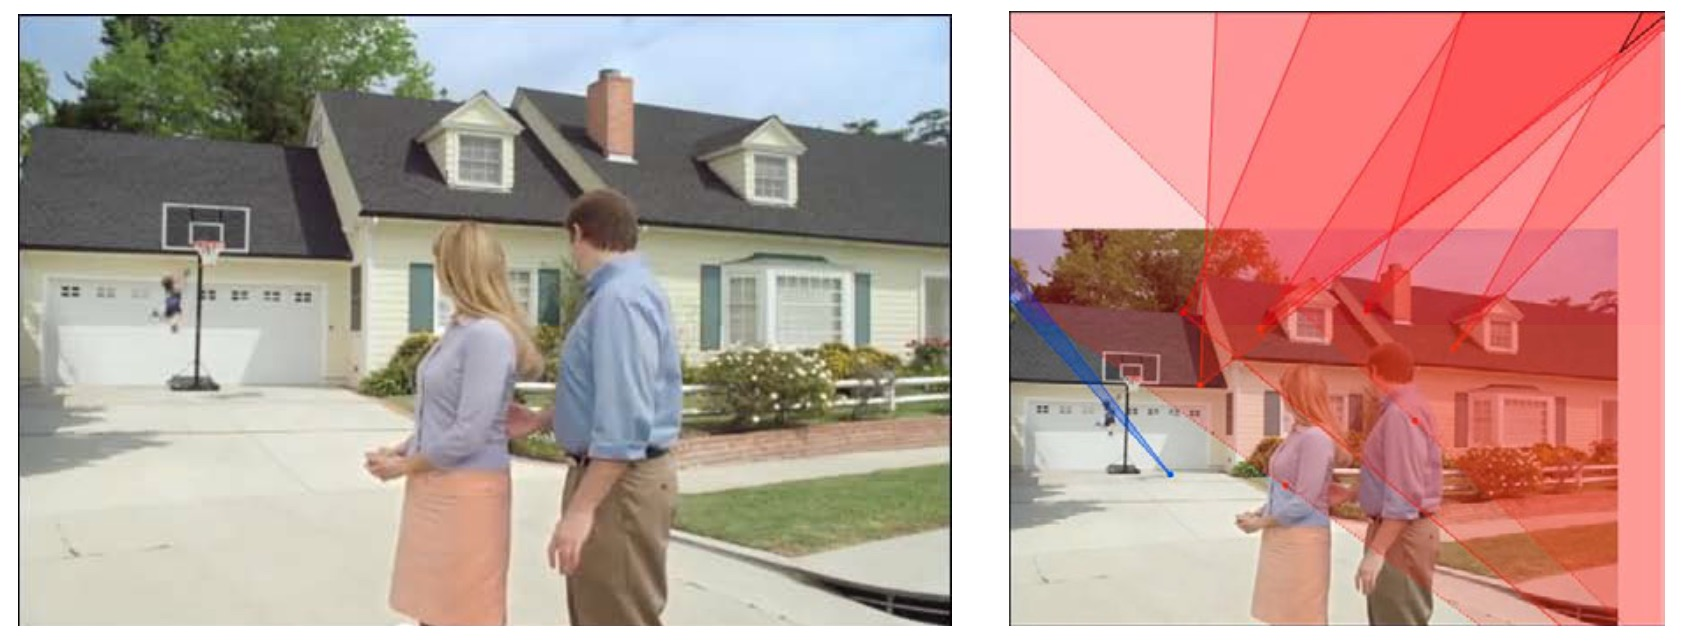
\includegraphics[width=0.8\textwidth]{shadows_inconsistencies}
    \caption{Original image (left) and the extracted shadows constraints (right)}
    \label{shadows_inconsistencies}
\end{figure}

The second constraint is based on the ratio of these connecting lines. In addition, the authors also proposed to explore the changing ratio along the normal direction of the shadow boundaries. 

Geometric and shadow photometric constraints together are used to detect image compositions. However, in spite of being a good initial step in forensic shadow analysis, the major drawback of the method is that it only works with images containing casting shadows, a very restricted scenario.

\subsection{Inconsistencies in light color}

The last group of methods investigate the presence, or not, of composition operations in digital images using color inconsistencies.

Gholap and Bora\cite{gholap2008illuminant}\cite{francis2014illuminant} pioneered this approach using the \emph{illuminant colors}. For that, the authors used a \emph{dichromatic reflection model} proposed by Tominaga and Wandell\cite{tominaga1989standard}, which assumes a single light source to estimate illuminant colors from images.

\begin{figure}
  \begin{center}
    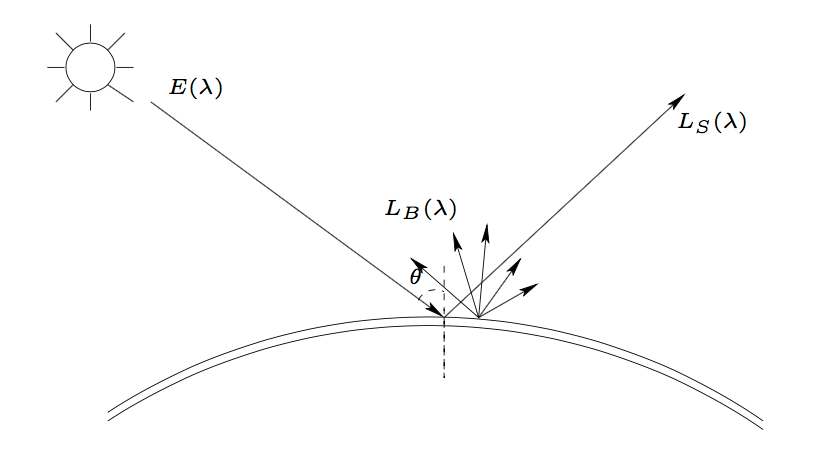
\includegraphics[width=0.65\textwidth]{dichromatic_reflection_model}
  \end{center}
  \caption{The dichromatic reflection model}
    \label{fig:dichromaticreflectionmodel}
\end{figure}


According to this model, the reflection of any non-homogeneous material may be modelled as additive mixture of two components, diffused reflection and surface reflection as shown in Fig. \ref{fig:dichromaticreflectionmodel}.

Considering an object point illuminated by a light source, the reflected ray consists of diffuse reflection $L_B (\lambda)$ and surface reflection $L_S (\lambda)$. The reflected light $L(\Theta, \lambda)$ can be written as:

\begin{equation} \label{eq:dichromaticmodel}
L(\Theta, \lambda) = m_S(\Theta) L_S(\lambda) + m_B(\Theta) L_B(\lambda)
\end{equation}

where $m_S(\Theta)$ and $m_B(\Theta)$ are geometrical factors and $\Theta$ the angle of the incident light. This equation can be rewritten in terms of RGB sensors in matrix form.

The two vectors $L_B(\lambda)$ and $L_S(\lambda)$ span the two dimensional plane called \emph{dichromatic plane}.

Dichromatic planes can also be estimated using principal component analysis (PCA) from each specular highlight region of an image. By applying a \emph{Singular Value Decomposition (SVD)} on the RGB matrix extracted from highlighted regions, the authors extract the eigenvectors associated with the two most significant eigenvalues to construct the \emph{dichromatic plane}. This plane is then mapped onto a straight line, named dichromatic line, in normalized \emph{r-g-chromaticity} space. 

For distinct objects illuminated by the same light source, the intersection point produced by their dichromatic line intersection represents the illuminant color. If the image has more than one illuminant, it will present more than one intersection point, which is not expected to happen in pristine (non-forged images). This method represented the first important step toward forgery detection using illuminant colors, but has some limitations such as the need of well defined specular highlight regions for estimating the illuminants.

Following Gholap and Bora’s work, Riess and Angelopoulou\cite{riess2010scene} used an extension of the \emph{Inverse-Intensity Chromaticity Space}, originally proposed by Tan et al.\cite{tan2004color}, to estimate illuminants locally from different parts of an image for detecting forgeries.

In addition, Wu and Fang\cite{wu2011image} proposed a new way to detect forgeries using illuminant colors. Their method divides a color image into overlapping blocks estimating the illuminant color for each block. To estimate the illuminant color, the authors proposed to use the algorithms Gray-World, Gray-Shadow and Gray-Edge \cite{van2007edge}.

These approaches will be better explained in the next section due their importance for this proposed method.

\section{Illuminant color estimation}


The color of an object observed in an image depends both on its intrinsic color and on the color of light source i.e., the illuminant. 

It is important to keep in mind that even the same light source can generate different illuminants. The illuminant formed by the sun, for example, varies in its appearance during the day and time of year as well as with the weather. We only capture the same illuminant, measuring the sunlight at the same place at the same time.

We can explore illuminants in forensics to check the consistency of similar objects in a scene. If two objects with very similar color stimuli (e.g., human skin) depict inconsistent appearance (different illuminants), it means  that they might have undergone different illumination conditions hinting at a possible image composition. On the other hand, if we consider a photograph with two people and the color appearance on the faces of such people are consistent, it is likely they have undergone similar lighting conditions.

Riess and Angelopoulou\cite{riess2010scene} pioneered the approach of using a color-based method that investigates illuminant colors to detect forgeries in forensic scenario. In their work, illuminant colors are estimated locally, effectively decomposing the scene in a map of differently illuminated regions. Inconsistencies in such a map suggest possible image tampering.

The method can be divided into four steps:

\begin{enumerate}
\item Image segmentation. The image is segmented into regions, called \emph{superpixels}, of approximately the same object color. Each superpixel must be:
\begin{enumerate}
\item Directly illuminated by the same light source.
\item Compliant with the \emph{dichromatic reflectance model}\cite{tan2004color}.
\end{enumerate}
\item Manual user selection of superpixels under investigation.
\item Local illuminant color estimation for each superpixel (both for segmented superpixels and user selected regions).
\item Reference illuminant selection (manual) and \emph{distance map} evaluation. The distance map is the base for an expert analysis for forgery detection.
\end{enumerate}

\begin{figure}
  \centering
    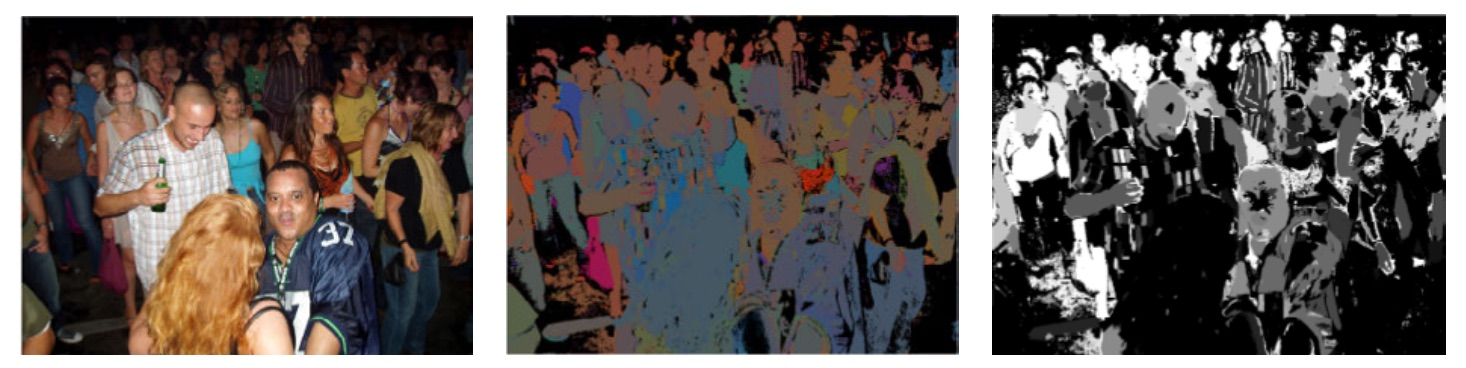
\includegraphics[width=.98\textwidth]{illuminant_maps}
    \caption{An example of a generated distance map using Riess and Angelopoulou\cite{riess2010scene} approach. From left to right: (a) the original image, (b) \emph{illuminant map}, (c) generated distance map}
    \label{illuminant_maps}
\end{figure}

The final decision of this approach is delegated to an expert and not to the algorithm itself.

\subsection{Illuminant maps}


\subsubsection{Generalized Greyworld estimation}

The starting point is the \emph{gray world assumption}, proposed by Buchsbaum\cite{Buchsbaum19801}. In its simplest version, it is assumed that information in the average of each channel of the image is the representative gray level.

Let $f(x) = (\Gamma_R(x), \Gamma_G(x), \Gamma_B(x))^T$ the RGB color of a pixel at position $x$ and $\Gamma_i(x)$ the intensity of that pixel in the $i$-th channel. In their paper, Van de Weijer et al. assumes that the camera response is linear. It is also assumed that the scene is illuminated by a single light source.

The RGB color $f(x)$ can also be rewritten as

\begin{equation}
f(x) = \int_{\omega} e(\beta, x) s(\beta, x) c(\beta) d\beta
\end{equation}

where $\omega$ is the visible light spectrum, $\beta$ is the light wavelenght, $e(\beta, x)$ is the illuminant spectrum, $s(\beta, x)$ is the surface reflectance of an object and $c(\beta)$ is the color sensitivity of the camera for each channel.

As an alternative to the gray-world hypothesis, Van de Weijer et al.\cite{van2007edge} proposed the \emph{gray-edge hypothesis}: the average of the reflectance differences in a scene is achromatic.

This idea led to a framework for low-level based illuminant estimation, called \emph{Generalized Grayworld}.

\begin{equation}\label{eq:ggeframework}
\left( \int 	\left | \frac{\delta^n f^{\sigma}(x)}{\delta x^{n}} \right |^{p} dx \right)^{\frac{1}{p}} = k e ^{n, p, \sigma}
\end{equation}

where $k$ denotes a scaling factor, $|\cdot|$ the norm operand, $\delta$ the differential operator and $f^{\sigma}(x)$ the pixel intensities at position $x$, smoothed with a Gaussian kernel $\sigma$.

The framework defined by (\ref{eq:ggeframework}) produces different estimations for the illuminant color based on three parameters:

\begin{enumerate}
\item The order $n$ determines if the method is a gray-world or a gray-edge algorithm. The gray-world methods are based on the RGB values, whereas the gray-edge methods are based on the spatial derivative of order $n$.
\item The Minkowski norm $p$ determines the relative weights of the multiple measurements from which the final illuminant color is estimated.
\item The scale $\sigma$ of the local measurements. For first or higher order estimation, this local scale is combined with the differentiation operation computed with the Gaussian derivative. For zero-order gray-world methods, this local scale is imposed by a Gaussian smoothing operation.
\end{enumerate}

On varying of these parameter, a different method can be used. An overview of the possible methods that derive from  Eq. (\ref{eq:ggeframework}) is displayed in Table \ref{table:ggemethods}.

\begin{table}[h!]
\caption{Overview of different illuminant estimation methods based on \ref{eq:ggeframework}}
\centering
\small
\begin{tabular}{l c c p{4.5cm}} 
\hline\hline 
Name & Symbol & Equation & Assumption \\ [0.5ex]
\hline 
Gray-World & $e^{0, 1, 0}$ & $(\int f(x) dx) = k e$ & The average reflectance in a scene is achromatic \\
max-RGB & $e^{0, \infty, 0}$ & $(\int |f(x)|^{\infty} dx)^{\frac{1}{\infty}} = k e$ & The maximum reflectance in a scene is achromatic \\
Shades of Gray & $e^{0, p, 0}$ & $(\int |f(x)|^{p} dx)^{\frac{1}{p}} = k e$ & The $p$-th Minkowski norm of scene is achromatic \\
General Gray-World & $e^{0, p, \sigma}$ & $(\int |f^{\sigma}(x)|^{p} dx)^{\frac{1}{p}} = k e$ & The $p$-th Minkowski norm of scene is achromatic after smoothing\\
Gray-Edge & $e^{1, p, \sigma}$ & $(\int |f^{\sigma}_{x}(x)|^{p} dx)^{\frac{1}{p}} = k e$ & The $p$-th Minkowski norm of the image derivative is achromatic\\
Max-Edge & $e^{1, \infty, \sigma}$ & $(\int |f^{\sigma}_{x}(x)|^{\infty} dx)^{\frac{1}{\infty}} = k e$ & The maximum reflectance difference in a scene is achromatic\\
2nd order Gray-Edge & $e^{2, p, \sigma}$ & $(\int |f^{\sigma}_{xx}(x)|^{p} dx)^{\frac{1}{p}} = k e$ & The $p$-th Minkowski norm of the second order derivative in a scene is achromatic\\ [1ex]
\hline
\end{tabular}
\label{table:ggemethods}
\end{table}

\subsubsection{Inverse Intensity-Chromaticity estimation}

The other considered illuminant estimation method is based on the idea proposed by Tan et al.\cite{tan2004color}, called \emph{inverse intensity-chromaticity}.

The base for this kind of approaches is the dichromatic reflectance model\cite{gholap2008illuminant}, which states that the amount of light reflected from a point, $x$, of a dielectric, non-uniform material is a linear combination of diffuse reflection and specular reflection. Further assumptions assume that the color of the specularities approximates the color of the illuminant, and that the camera response is linear.

Considering a trichromatic camera, the sensor response $I_c (x)$, for each color channel $c \in \{R, G, B\}$ is:

\begin{equation}\label{eq:sensorrespiic}
I_c(x) = m_{S}(x) L_{S_c}(x) + m_B(x) L_{B_c}(x)
\end{equation}

as described in \ref{eq:dichromaticmodel}. 

Let $\sigma_c$ the image chromaticity, $\Delta_c(x)$ the diffuse chromaticity and $\Gamma_c(x)$ the specular chromaticity defined as follows:

\begin{equation}
\sigma_c(x) = \frac{I_c(x)}{\sum_i I_i(x)} \textrm{  where } i \in \{R, G, B\}\
\end{equation}
\begin{equation}
\Delta_c(x) = \frac{L_{S, c}(x)}{\sum_i L_{S, i}(x)} \textrm{  where } i \in \{R, G, B\}\
\end{equation}
\begin{equation}
\Gamma_c(x) = \frac{L_{B, c}(x)}{\sum_i L_{B, i}(x)} \textrm{  where } i \in \{R, G, B\}\
\end{equation}

Thus the Eq. \ref{eq:sensorrespiic} can be rewritten as

\begin{equation}
I_c(x) = m_S(x) \Delta_c(x) + m_B(x) \Gamma_c(x)
\end{equation}

Tan et al.\cite{tan2004color} derived a linear relationship between diffuse, specular and image chromaticities:

\begin{equation}
\sigma_c(x) = m(x) \frac{1}{\sum_{i} I_i(x)} + \Gamma_c(x)
\end{equation}

where $i \in \{R, G, B\}$ and $m(x)$ is a geometrical factor (light position, surface orientation, camera position, ...), that can be approximated. In the illuminant estimation, the most important aspect is the $y$-intercept $\Gamma_c$.

\begin{figure}
  \centering
    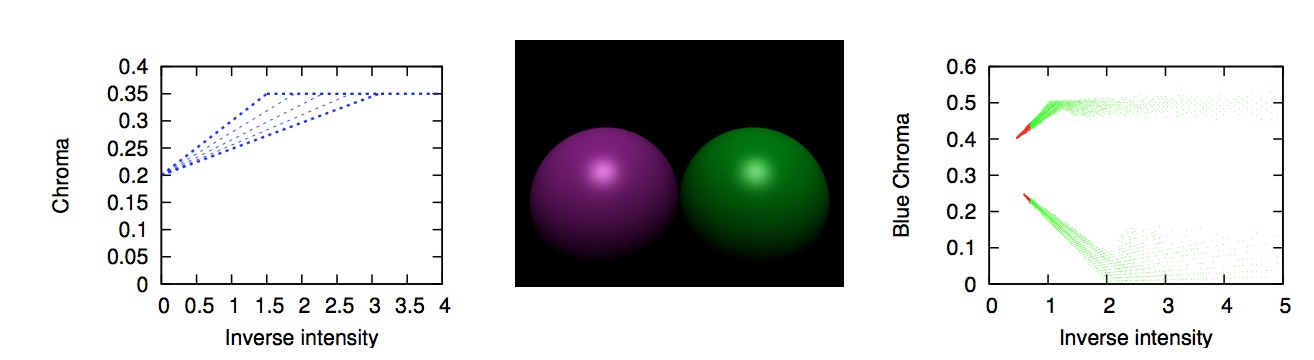
\includegraphics[width=1\textwidth]{iic_space}
    \caption{Pixel distribution in inverse-intensity chromaticity (IIC) space. Left are as ideal distribution, right on a synthetic image (in the center).}
    \label{fig:iic_space}
\end{figure}

The 2D space defined by $\frac{1}{\sum_{i} I_i(x)}$ as domain and $0 \leq \sigma_c \leq 1$ as range is called \emph{inverse-intensity chromaticity (IIC)} space.

An example of the IIC plots for a single channel of a synthetic image is shown in Fig. \ref{fig:iic_space}.
Pixels from the green and purple balls form two clusters. The clusters have spikes that point towards the same location on the $y$-axis. Considering only such spikes from each cluster, the illuminant chromaticity is estimated from the joint $y$-axis intercept of all spikes in IIC space.

Instead of examining the entire pixel distribution, Riess et al.\cite{riess2010scene} perform the analysis over small connected image regions of roughly uniform object color (\emph{superpixels}). Depending on the outcome of our shape analysis, we can either use this local region to obtain an illuminant estimate, or reject it if it does not seem to fulfill the underlying assumptions of the proposed model. Using local regions allows us to incorporate multiple sampling and voting in the estimation of local illuminants.

\section{Human faces splicing detection}

The approach proposed in Chapter 2 is based on two different works, published by Carvalho et al.\cite{carvalho2016illuminant} and Fan et al.\cite{fan2015image}.

The method proposed by Carvalho et al.\cite{carvalho2016illuminant} aims to detect splicing focusing on human faces, minimizing the user interaction. Faces are previously labeled by a human selecting the box within is contained, than the process will associate a label to each face (i.e. \emph{normal} or \emph{fake}).

The method can be divided into four steps:

\begin{enumerate}
\item \emph{Description}: in this step illuminant maps are estimated with the two different approaches, GGE and IIC, and feature vectors are generated. Each feature vector is associated with a face pair.
\begin{figure}[h!]
  \centering
    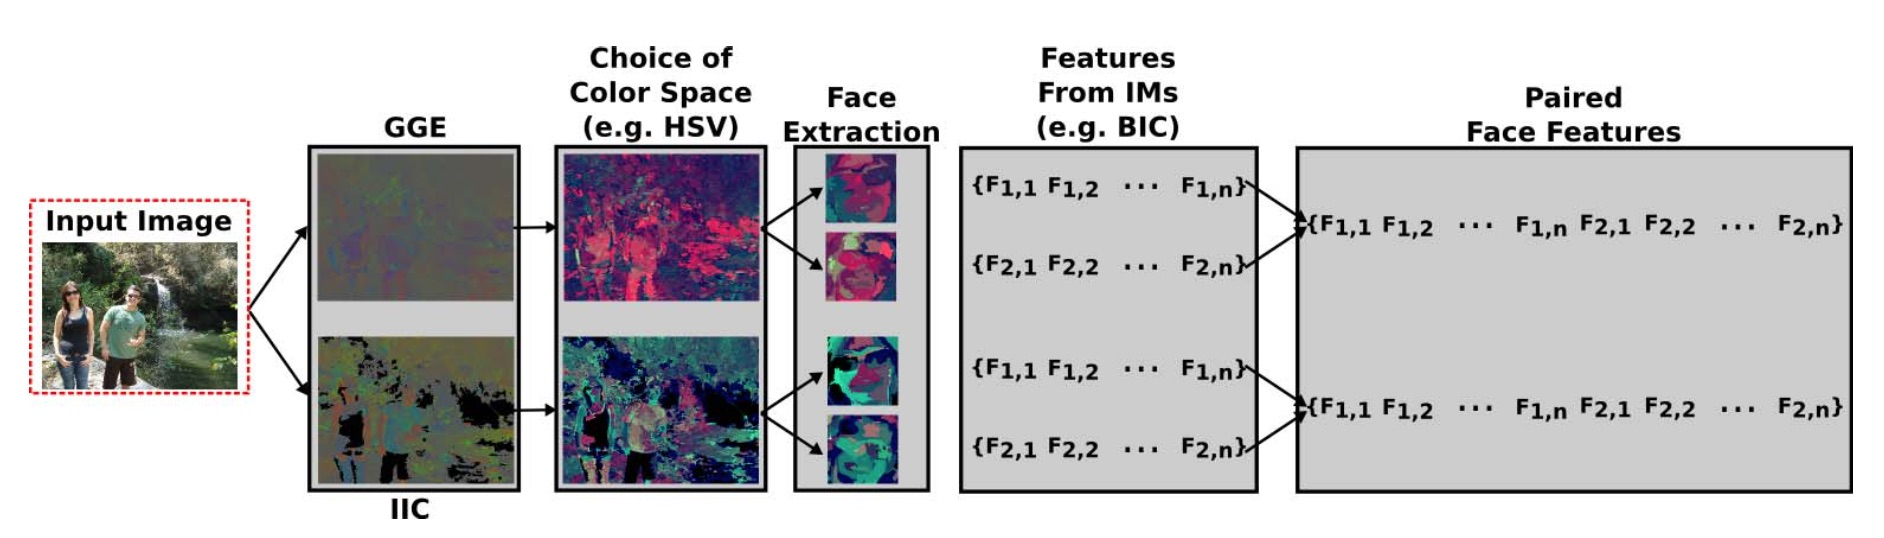
\includegraphics[width=1\textwidth]{tiago_method_extraction}
    \caption{Image description pipeline for extracting paired face feature vectors}
    \label{fig:tiago_method_extraction}
\end{figure}

The Fig. \ref{fig:tiago_method_extraction} shows the image description extraction pipeline. Given an input image, the illuminant maps are estimated and converted to a selected color space (e.g. HSV). So, the faces in the image are extracted (using the defined area). For each face a descriptor is used to generate a feature vector (e.g a color descriptor, texture descriptor or shape descriptors) and finally they are coupled in order to generate paired feature vector simply concatenating the two original vectors.

In this step multiple descriptors and color spaces are used in order to increment the number of final classifiers.

\item \emph{Face Pair Classification}: a set of classification models are trained using the previous step feature vectors. Based on the number of color spaces and descriptors used, a set of KNN classifiers are trained over the paired face feature vectors. The final result is given by a majority voting of all the selected classifiers.

\item \emph{Forgery Classification}: given an image $I$ containing $q$ people (faces), it is characterized by a set $\mathcal{S} = \{\mathcal{P}_1, \ldots, \mathcal{P}_m \}$, where $\mathcal{P}_i$ is the $i$-th paired feature vector and $m = \frac{q(q-1)}{2}, q \geq 2$. If any $\mathcal{P}_i \in \mathcal{S}$ is classified as fake, the image $I$ is classified as fake. Otherwise, the image is considered as pristine.

\item \emph{Forgery Detection}: once knowing that an image is fake, in this stage it is identified which one is more likely to be fake in the image. This is done using a specific SVM classifier.   
\end{enumerate}

\begin{figure}[h!]
  \centering
    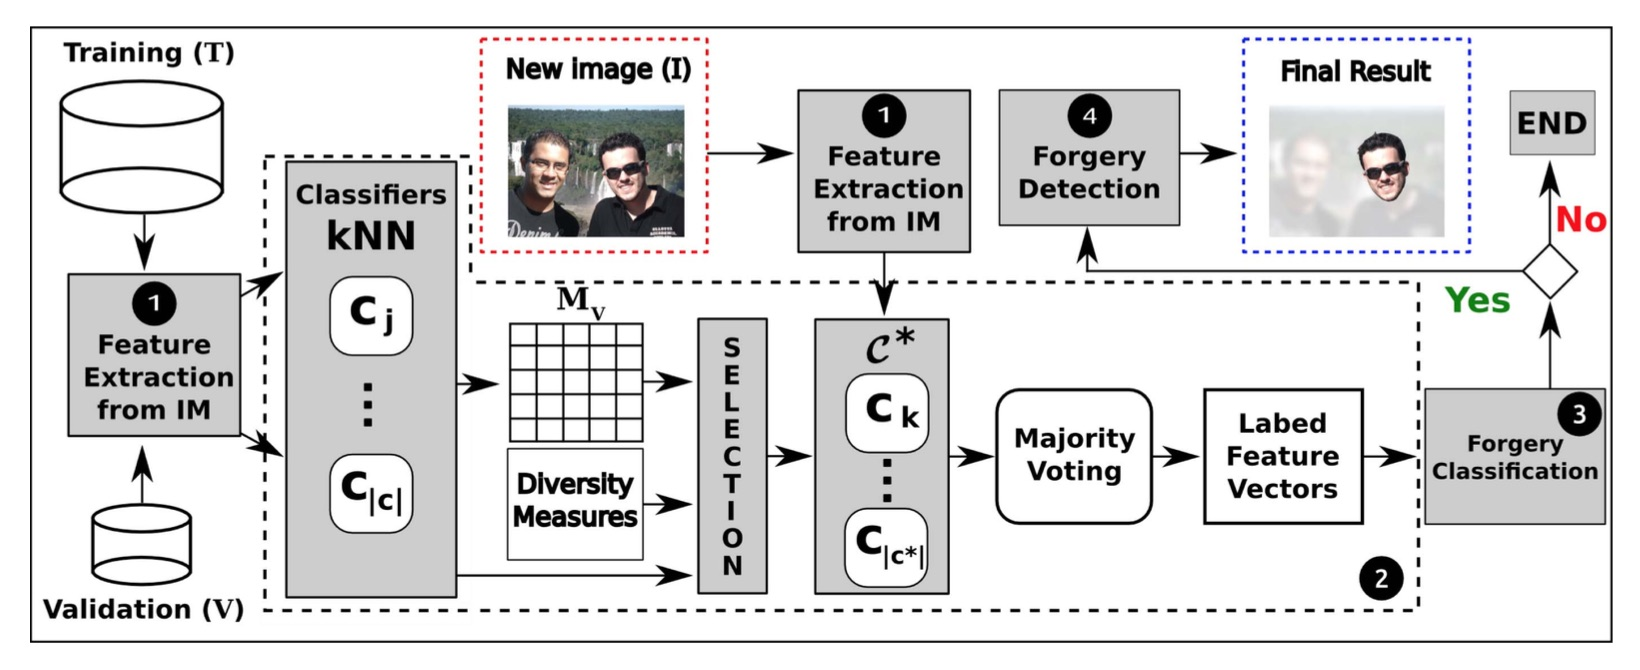
\includegraphics[width=1\textwidth]{tiago_method_full}
    \caption{Image splicing detection over human faces}
    \label{fig:tiago_method_full}
\end{figure}

The Fig. \ref{fig:tiago_method_full} shows the above descripted method pipeline.

\subsection{Method drawbacks}

The main drawback of this approach relies in the manual selection of faces by a human agent. The definition of a face in the image by the operator is made by identification of the bounding box in which it is fully contained.

This manual operation does not allow a blind approach to the problem. Because the faces are considered in pairs, this method can be applied only in the case when there are at least two faces, so you need to know in advance the content of the images to assess the applicability of this algorithm.

Working with pairs of faces, another problem is the choice of which face has been manipulated among those considered. 

In addition, this method is based on the observation that, given two faces (a pristine face and a spliced one), the difference between the two forged faces illuminant maps tend to be higher. This intuition, however, proved to be not applicable in all contexts, so cannot be considered as a starting point for the final evaluation.

\section{Region splicing detection}

The other considered approach is based on the work of Fan et al.\cite{fan2015image}. This method relies on the Van de Weijer et al.\cite{van2007edge} Generalized Gray-World framework \ref{eq:ggeframework} in Eq. \ref{eq:ggeframework}. This algorithm performs better on a scene when it is rich of colors, but in a splicing detection scenario we are interested in a specific region of the image.

This approach splits the image in vertical and horizontal bands (rectangular regions), assuming that each band contains sufficient colors for a correct illuminant estimation. Five different algorithms are used, deduced from Eq. \ref{eq:ggeframework}: Grey-World, Max-RGB, Shades of Grey, first- order Grey-Edge and second-order Grey-Edge, in order to have as many illuminant estimates for each band.

This algorithm can be divided into two steps:
\begin{enumerate}
\item Subsampling of the image horizontally and vertically;
\item Illuminant estimation for each band using the 5 different algorithms and spliced region location.
\end{enumerate}

In the first step the image is sampled into two band categories: horizontal and vertical bands. The height and the width of each band is configured \emph{a priori} based on the minimal height and minimal width separately among the objects of interest. An object of interest is encompassed by a virtual rectangle with its height and width decided by the object itself.

The second step can be also divided into five steps:

\begin{enumerate}
\item For each direction and for each algorithm, a reference illuminant is estimated for a single band.
\item For each direction and for each algorithm, a reference illuminant for each direction is evaluated as the median of all references of that direction. At this stage there are two reference illuminants (one for the vertical and one for the horizontal direction) for each algorithm.
\item A detection map is created, with the same dimensions of the image.
\item For each algorithm, every band estimate is compared with the reference illuminant of that band direction and algorithm with the Euclidean distance. If the distance exceeds a fixed threshold, the band is considered fake and all the pixel values in the detection map are increased by one unit.
\item The forgery is located using the resulting thresholded detection map.
\end{enumerate}

\begin{figure}[h!]
  \centering
    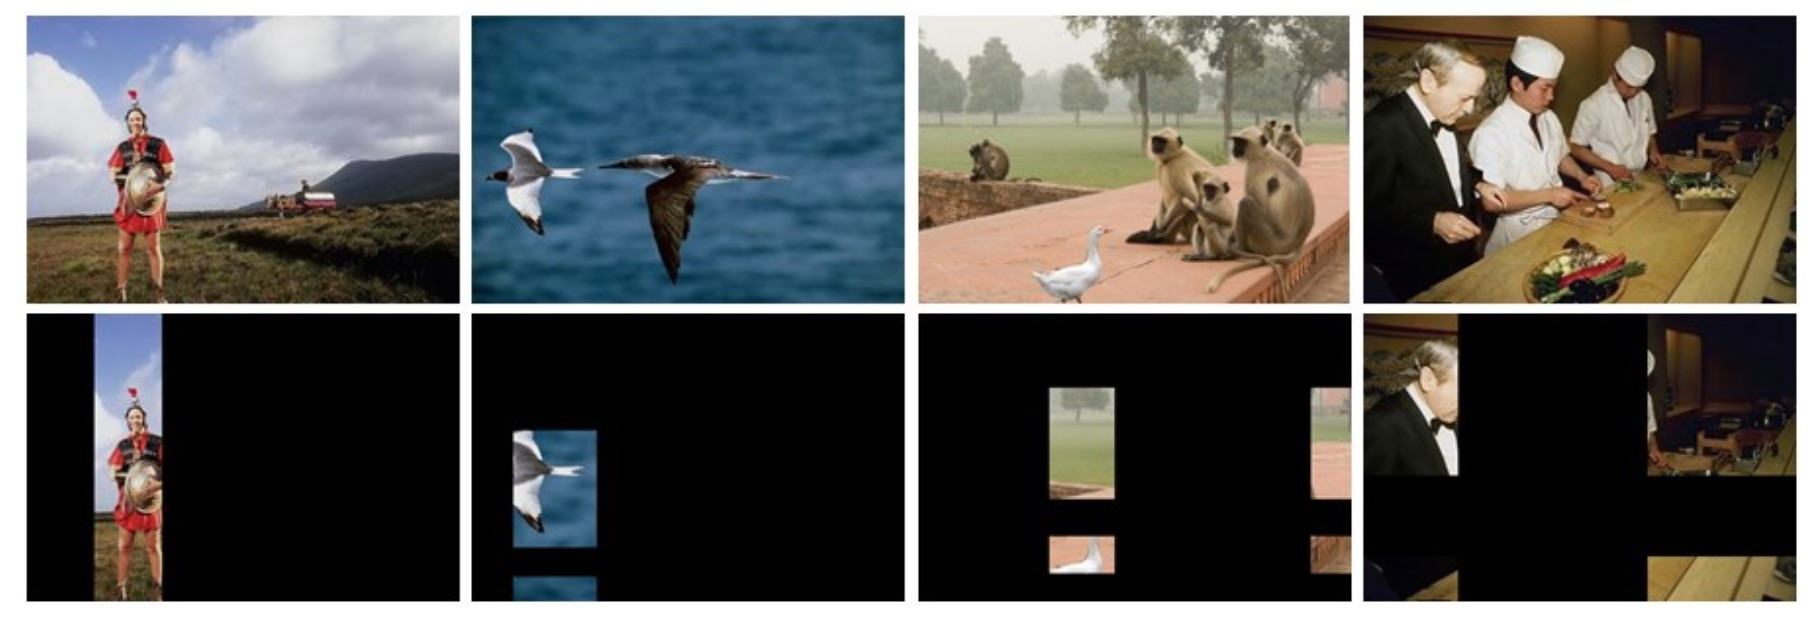
\includegraphics[width=1\textwidth]{regionsmethod}
    \caption{Image regions splicing detection}
    \label{fig:regionsmethod}
\end{figure}

The main advantage of this method is its blind approach: the algorithm is not based on the image content (as it was in the previous case) and no human interaction is needed. The only parameters are the bands minimal dimensions and the threshold. Due these facts it is very simple to implement.

\subsection{Method drawbacks}

Due its simplicity, this approach has some drawbacks. First, because the classification is based on a simple distance between a reference value, a key point is the identification of optimal thresholds.

These thresholds can be calculated experimentally, but their accuracy will depend on the dataset with which they were computed.

For how it's built, moreover, this method tends to have a low detection rate compared to a high false positive rate.
\chapter{Proposed approach}

In the previous chapter, a review of two splicing detection methods based on illuminant colors analysis has been presented. However, their effectiveness still need to be improved for real forensic applications.

The approach proposed in this chapter has been developed to correct some of the two approaches drawbacks and mainly to combine them together in order to realize a more general algorithm for image forgery detection. 

\section{Overview}

Most of the times, the splicing detection process relies on the expert's experience and background knowledge. This process usually is time consuming and error prone once that image splicing is more and more sophisticated and an aural (e.g., visual) analysis may not be enough to detect forgeries.

This approach to detecting image splicing is developed aiming at minimizing the user interaction. 

The two methods, presented in the previous chapter \cite{carvalho2016illuminant} and \cite{fan2015image}, are now being used in synergy with each other, going to analyze the suspicious image at the same time looking for potential signs of forgery.

Starting from an image we want to analyze, the method will output a set of results.
\begin{itemize}
\item A classification \textbf{label} indicating whether an image is believed to be original or counterfeit.
\item A classification \textbf{score} indicating the confidence of the algorithm output.
\item A \textbf{detection map} highlighting the detected spliced regions.
\end{itemize}

The proposed approach minimizes the needed human interaction and aims at being a fully automated process. However, not both the modules can operate in any circumstance. The face splicing detection module will work only if there is a number of faces greater than or equal to two.

\section{Face splicing detection module}

The first module consists in the implementation, with few enhancements and simplifications, of the method proposed by Carvalho et al. \cite{carvalho2016illuminant} and presented in Section 1.6.

The algorithm can be used on an image that contains at least two human faces, looking for inconsistencies in the illuminant color in presence of human skin. In particular, in case of a forgery detection, the algorithm tries to guess which faces in the images are doctored.

The algorithm requires an initial training phase, so a dataset with annotated human faces is needed. 

This module consists of 4 consecutive stages:

\begin{enumerate}
\item \textbf{Illuminant maps extraction}: given an input image, two different illuminant maps are evaluated, using the IIC and GGE extraction methods.
\item \textbf{Face detection}: after the illuminant maps extraction, the human faces in the image are detected. In the training phase the faces positions are read from the groundtruth file. If the given image contains less than two faces, it is discarded.
\item \textbf{Paired face feature extraction}: human faces are considered and classified in pairs. From each extracted face in the previous step, a color descriptor is used in order to extract features.
\item \textbf{KNN models training}: fixed a value of $K$, a set of KNN models are trained using previous feature vectors.
\item \textbf{Forgery detection and classification}: in this step an image is classified as fake or normal. Given an image classified as fake, the analysis is refined pointing out which face of the image is the result of a composition.
\end{enumerate}

\subsection{Illuminant maps extraction}

Given a single image $I$ the two different illuminant maps are extracted: both generalized grayworld algorithm (GGE) and inverse-intensity chromaticity estimation (IIC) are used.

\begin{figure}[!htb]
\minipage{0.32\textwidth}
  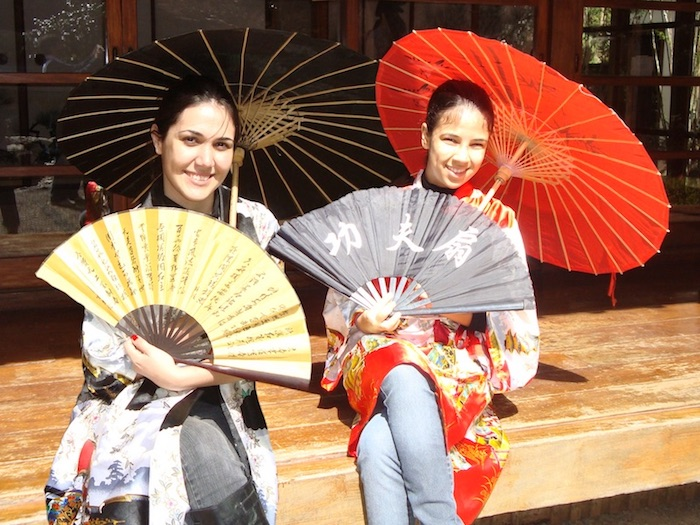
\includegraphics[width=\linewidth]{splicing-33.jpg}
  \caption{The original image}\label{fig:awesome_image1}
\endminipage\hfill
\minipage{0.32\textwidth}
  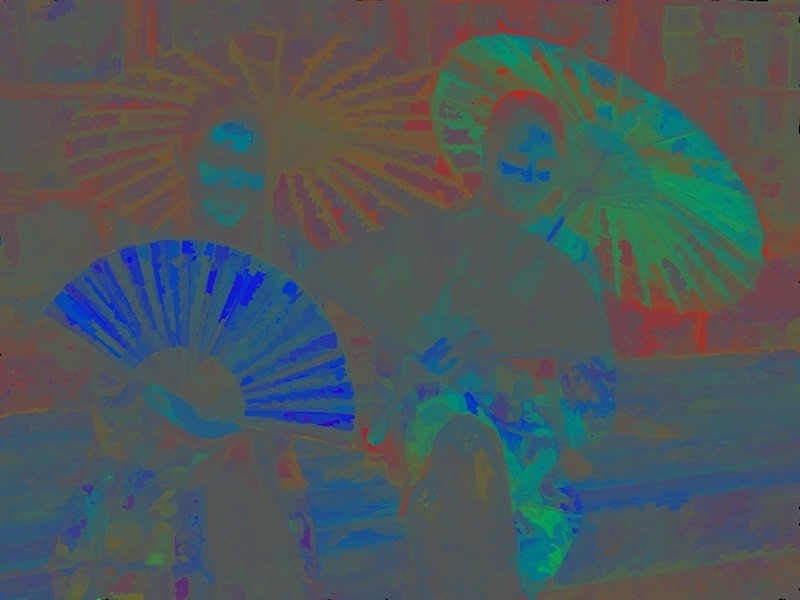
\includegraphics[width=\linewidth]{splicing-33_gge_map.jpg}
  \caption{GGE illuminant map}\label{fig:awesome_image2}
\endminipage\hfill
\minipage{0.32\textwidth}%
  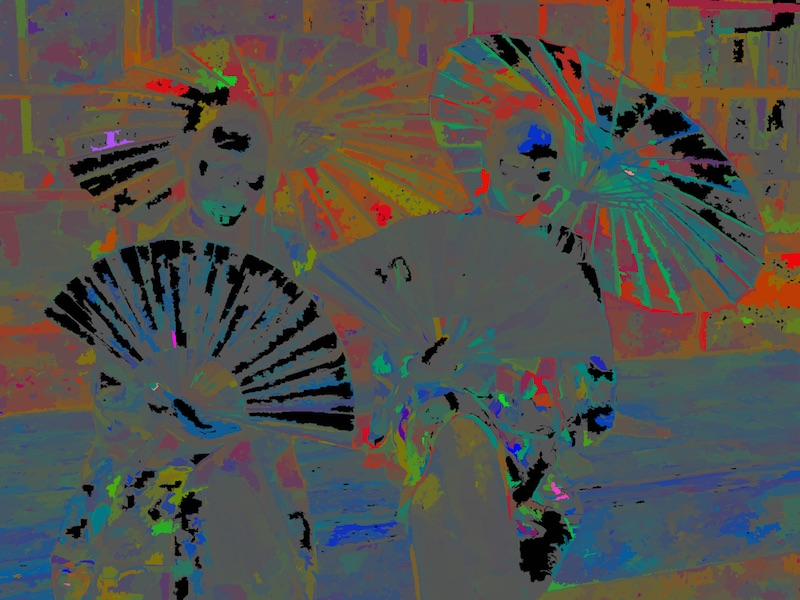
\includegraphics[width=\linewidth]{splicing-33_iic_map.jpg}
  \caption{IIC illuminant map}\label{fig:awesome_image3}
\endminipage
\end{figure}

Differently from de Carvalho et al. \cite{carvalho2016illuminant}, who have used the conversion of IMs to the YCbCr color space, the two IMs are considered as two different color maps theirself.

The illuminant maps extraction algorithm implementation used is the one proposed by Riess et. al. for \cite{riess2010scene} and downloadable in the project page\footnote{Homepage of the project \cite{riess2010scene} - www5.cs.fau.de/research/areas/computer-vision/image-forensics/scene-illumination-as-an-indicator-of-image-manipulation}. The code provides an implementation of both of the two illuminant map extraction methods, using a local estimation approach.

\subsection{Face detection}

One of the drawback of the method proposed by Carvalho et al. \cite{carvalho2016illuminant} relies on the user interaction needed for detecting human faces in the image. In this approach a common face detection module is used to achieve the same results, aiming at minimizing the user dependency and making the entire algorithm user independent.

The face detector used is the one initially proposed by Viola and Jones \cite{viola2001rapid}\cite{viola2004robust} and improved by Lienhart et al. \cite{lienhart2002extended}. Usually called simply \emph{Viola-Jones}, its original motivation was face detection, but it can be trained to detect different object classes. 

This detector combines four key concepts: 
\begin{itemize}
\item Simple rectangular features, called \emph{Haar features}
\item \emph{Integral Image}\cite{crow1984summed} concept for rapid feature detection 
\item \emph{AdaBoost}\cite{freund1995desicion} machine-learning method 
\item A \emph{cascade classifier} to combine all features efficiently 
\end{itemize}

The used rectangle combinations are not true \emph{Haar wavelets}\cite{haar1910theorie}. Instead, they contain better suited rectangle combinations used for visual object detection. The presence of a Haar feature is determined by subtracting the pixel values of the dark region to the pixel values of the light one. If the difference exceeds a threshold value set during the training process, the feature is said to be present. 

\begin{figure}[h!]
  \centering
    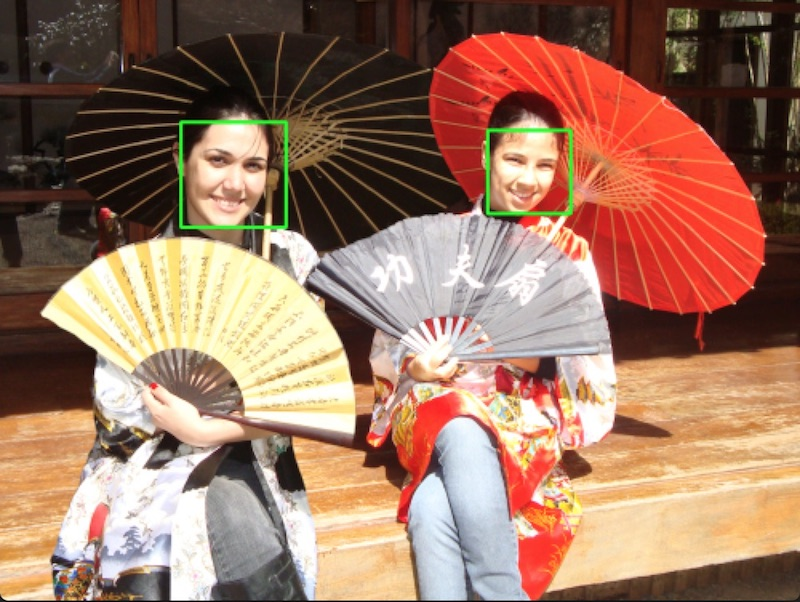
\includegraphics[width=0.5\textwidth]{facedetected}
    \caption{The output of the face detection module}
    \label{fig:facesdetected}
\end{figure}

\emph{OpenCV}\footnote{OpenCV - Open source computer vision. http://opencv.org} provides an implementation of the Viola-Jones face detector as \emph{cvHaarDetectObjects}.

Figure \ref{fig:facesdetected} shows the output of the face detector module. Given the output faces bounding boxes, the corresponding regions in the illuminant maps are extracted, Figure \ref{fig:facesdetectedmaps}.

\begin{figure}[h!]
  \centering
    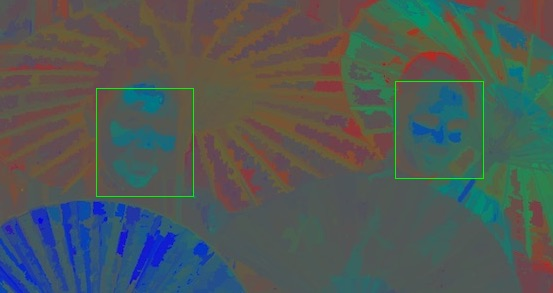
\includegraphics[width=0.5\textwidth]{splicing-33_gge_map_faces}
    \caption{The extracted faces from illuminant map}
    \label{fig:facesdetectedmaps}
\end{figure}

\subsection{Paired face feature extraction}

From each extracted face in the previous step, we need to find telltales that allow identification of spliced images. 

According to Riess and Angelopoulou \cite{riess2010scene}, when the output illumination maps are analyzed by an expert for detecting forgeries, the main observed feature is color. Thus, differently from Carvalho et al. \cite{carvalho2016illuminant} who have explored a large set of descriptors of different visual properties (e.g., texture, shape, color, among others) we focused our attention on color descriptors.

The considered color description techniques are ACC \cite{huang1997image}, BIC \cite{stehling2002compact}, CCV \cite{pass1997comparing}, and LCH \cite{swain1991color}.

\subsubsection{ACC descriptor}

\emph{Color Autocorrelogram (ACC) }\cite{huang1997image} maps the spatial information of colors by pixels correlations in different distances. Let $I$ an image, the \emph{autocorrelogram} (the term \emph{“correlogram”} is adapted from spatial data analysis \cite{upton1985spatial}) computes the probability of finding two pixels in $I$ with a color $c$ in a distance $d$ from each other. 

After the autocorrelogram computation, a set of $m$ probability values for each distance $d$ are considered, where $m$ stands for the number of colors in the quantized space. 

The implemented version quantized the RGB color space into 64 bins and considered 4 distance values (1, 3, 5, and 7). The \emph{L1} distance function is used.

\subsubsection{BIC descriptor}

\emph{Border/Interior Pixel Classification (BIC)} \cite{stehling2002compact} is a region-based color descriptor. Its extraction algorithm classifies the image pixels in border or interior
pixels. 

The image is first quantized into 64 colors in RGB color space. Then, each pixel is classified as interior
if its neighbors (above, below, left and right pixels) have the same color. Otherwise it is classified as border pixel. After the classification, two histograms are generated: one for border pixels and other for interior pixels. These histograms are stored as one single histogram with 128 bins.

\subsubsection{CCV descriptor}

\emph{Color Coherence Vector (CCV)} \cite{pass1997comparing} is a very popular color descriptor in the literature. Its extraction algorithm classifies the image pixels in coherent or incoherent pixels. This classification considers if the pixel belongs or not to a region with similar colors, called \emph{coherent region}. After the classification, two color histograms are computed: one for coherent pixels and other for incoherent pixels.

Both histograms are concatenated to compose the final feature vector. The RGB color space is quantized into 64 bins and L1 distance function is used.

\subsubsection{LCH descriptor}

\emph{Local Color Histogram (LCH)} \cite{swain1991color} is one of the most popular descriptors that is based on fixed size regions to describe image properties. Its extraction algorithm splits the image into fixed size blocks and computes a color histogram for each region. After that, the histograms of each region
are concatenated to compose one single histogram. 

The implemented version splits the image
in 16 regions (4x4 grid) and quantized the RGB color space into 64 bins. This generated feature vectors with 1024 values. The L1 distance function is used.


\subsubsection{Paired features}

In order to detect a face forgery, we need to compare the current analyzed image region against other, looking for color inconsistencies. Thus, instead of considering each face separately, faces are encoded in pairs.

Given two face feature vectors of the same type (i.e. extracted with the same color descriptor), $\mathcal{D}_1$ and $\mathcal{D}_2$, whose length depends on the color descriptor used, the final descriptor is computed concatenating them into a single feature vector $\mathcal{P}$. So, in an image $I$ containing $q$ faces, a set $S$ of feature vectors are extracted, with

$$
S = \{\mathcal{P}_1, \ldots, \mathcal{P}_m\} \quad \textrm{  where } m = \frac{q (q-1)}{2}
$$

if $q \geq 2$. 

Each paired face descriptor is computed twice for each considered color descriptor, one based on the GGE map and one based on the IIC map.

\subsection{KNN models training}

After the feature vectors are extracted from all faces in the images, a set of 8 \emph{k-nearest neighbors} binary classifiers are trained, 4 models based on the GGE map and 4 based on the IIC map. 

These models will be used in the classification step with majority voting. Given a paired  face feature vector $\mathcal{P}$ and the detection score is the result of the sum of all the prediction values of the classifiers:

$$
Score_{\mathcal{P}} = \sum_{i = 1}^{8} prediction_{C_i}(\mathcal{P}) \quad \textrm{ where } prediction_{C_i}(\mathcal{P}) \in [0, 1]
$$

Then $\mathcal{P}$ is considered as fake if its score is higher than a given threshold. 

\subsection{Forgery detection and classification}

Differently from Carvalho \emph{et al.} \cite{carvalho2016illuminant}, we used a different approach for classifying the single face as fake using the results of the paired face classification. 

Let $P_{i, j}$ the paired feature vector computed concatenating the $i$-th and the $j$-th face feature. If $P_{i, j}$ is classified as fake, the scores of the considered images are incremented by one unit. At the end of the process, faces with a higher associated scores have been classified as fake multiple times.

The resulting scores are then thresholded for selecting the most probably doctored faces. 

Given an input image $I$ containing $q$ faces, the forgery detection algorithm is summarized in Algorithm \ref{alg:faceforgerydetection}.

\begin{algorithm}[!h]
\begin{algorithmic}[1]
\State $Score_i = 0 \qquad \forall i \in Faces$ 
\For {$im \in \{GGE, IIC\}$}
\For {$desc \in \{ACC, BIC, CCV, LCH\}$}
\State $F = extractFeatures(im, desc)$
\State So $F = \{\mathcal{P}_1, \ldots, \mathcal{P}_m\} $ where $ m = \frac{q(q-1)}{2}$
\For {$f \in F$}
\State $prediction = KNN.predict(f)$
\If {$prediction = Positive$}
\State Let $i, j$ the faces considered for $f$ evaluation
\State Increment $i, j$ scores by $prediction \in [0, 1]$
\EndIf
\EndFor
\EndFor
\EndFor
\For {$i \in Faces$}
\If {$Score_i > Threshold$}
\State Mark $i$ as \emph{fake}
\EndIf
\EndFor
\end{algorithmic}\caption{Face forgery detection}\label{alg:faceforgerydetection}
\end{algorithm}

The output of the detector is a resulting detection mask, which highlights the spliced part of the image.

\begin{figure}[h!]
  \centering
    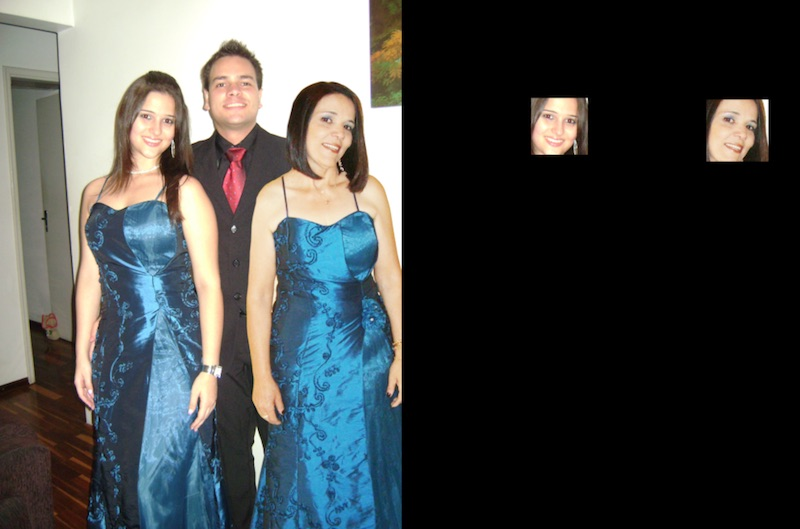
\includegraphics[width=0.55\textwidth]{facesplicingdetectionoutput}
    \caption{The output splicing detection module}
    \label{fig:facesplicingdetectionoutput}
\end{figure}

An example is shown in Figure \ref{fig:facesplicingdetectionoutput}. The two women in the image are counterfeited and their faces are shown in the resulting detection map as fake. In this particular case the detector has a perfect accuracy. 

\section{Region splicing detection module}

The second form of the algorithm is to implement the method proposed by Fan et al.\cite{fan2015image} with some changes in order to try to correct some of its major drawbacks presented in Section 1.7.

The splicing detection task performed by our approach consists in labelling a new image among two pre-defined classes (real and fake) and later pointing the face with higher probability to be the fake face. In this process, a classification model is created to indicate the class to which a new image belongs.

In summary, this module consists of the 6 main steps:

\begin{itemize}
\item \textbf{Image segementation}: relies on vertical and horizontal image segmentations. The outputs of this stage are two set of directional image bands. 
\item \textbf{Band illuminant estimation}: consists in estimating the illuminant color for each segmented band using 5 different GGE algorithms.
\item \textbf{Reference illuminant estimation}: consists in estimating the illuminant reference value for each direction.
\item \textbf{Feature vector evaluation}: relies on encoding the singular band illuminant information into a feature vector for further classification. The feature vector elements are the differences between the current illuminant color and the reference one.
\item \textbf{Band classification}: consists in labelling each image band into one of the know classes (real or fake) based on the previously learned classification model.
\item \textbf{Detection map}: using the classification output of the previous step, a detection map is build. The higher the value of this map, the higher the  resulting classification score for a single pixel.
\end{itemize}

\begin{figure}[h!]
  \centering
    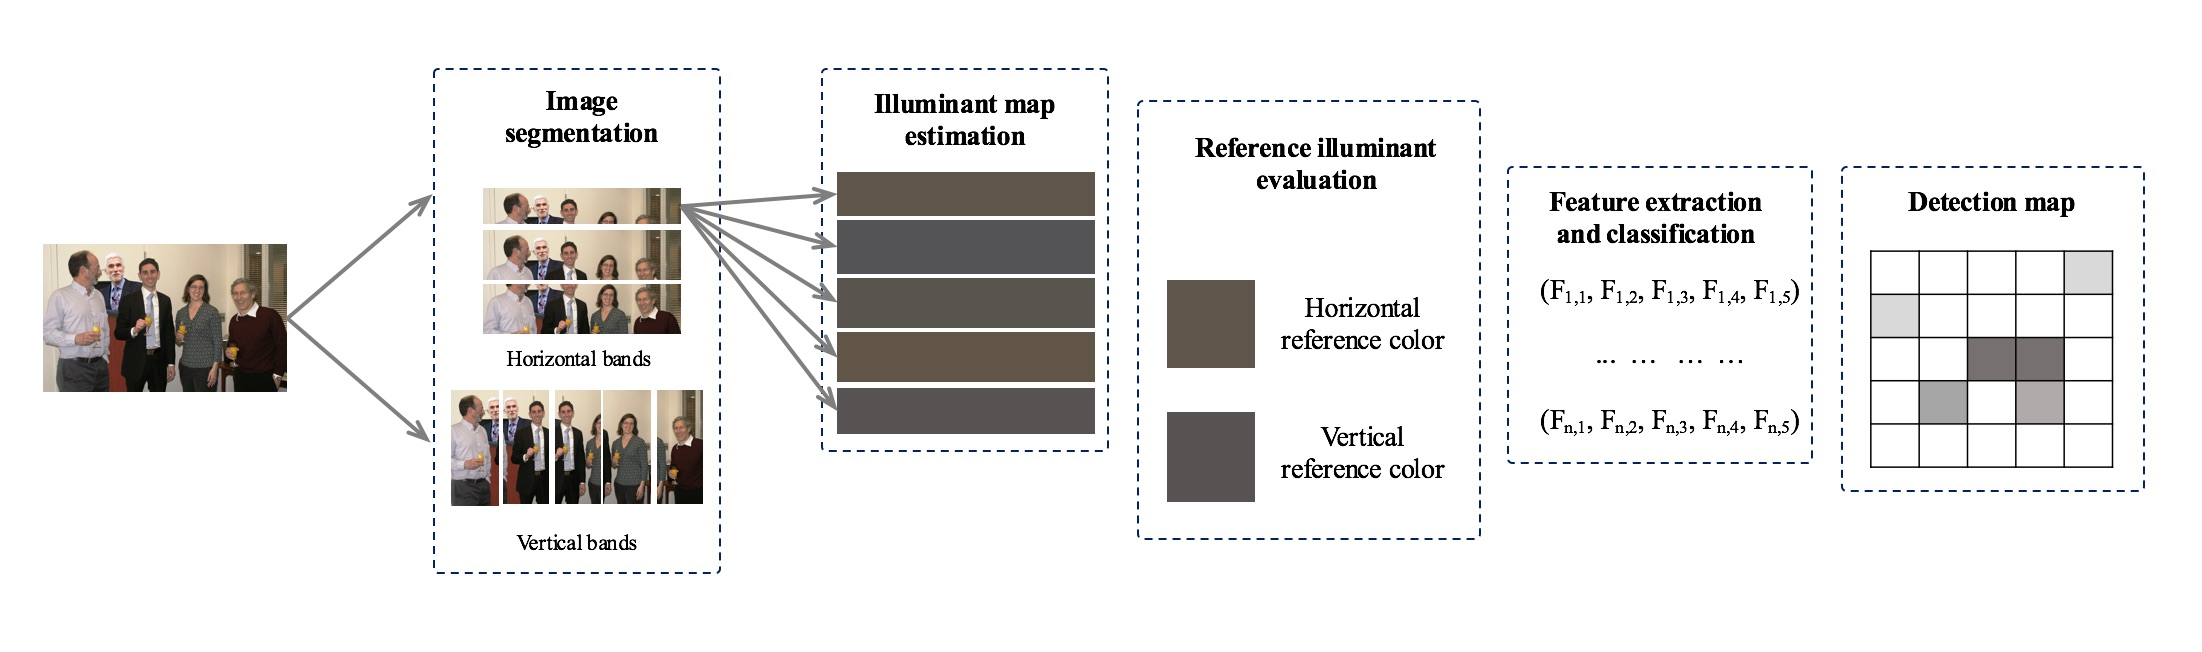
\includegraphics[width=1\textwidth]{pipeline_regions}
    \caption{Image regional splicing detection module pipeline}
    \label{fig:regionsmodulepipeline}
\end{figure}

The Fig \ref{fig:regionsmodulepipeline} summarize the module pipeline.

\subsection{Image segmentation}

In the first step of the process, the input image is segmented in order to obtain two image bands categories: horizontal and vertical bands. This kind of segmentation method is chosen because of its simplicity.

First, a band width $B_w$ and a band height $B_h$ is set. Due to the fact that the segmentation has to produce overlapping bands, we set a delta factor of $\frac{1}{4}$. As a result we get overlapping stripes for a total of 25\% of their area. 

The choice of the band size is a crucial phase of the algorithm: a band too tight would fail to capture the information necessary to classify our object of interest as falsified, unlike a band too wide would capture instead too much additional information.

The choice of the overlapped area percentage makes possible a more detailed evaluation. In this way it is possible to classify the same region of the image more than once, increasing the expressive power of our final classifier, the detection map.
 
In summary, let $I$ be the input image. After the segmentation process we obtain a set $B$ of bands containing all vertical and horizontal bands:

$$
B = \{V_1, \ldots, V_n, H_1, \ldots, H_m\}
$$

The dimension of $B$ is given by the sum of the number of vertical ($n$) and horizontal ($m$) bands.

\subsection{Band illuminant estimation}

The resulting image bands are now processed in order to evaluate the illuminant color using different techniques.

For this step, the Generalized Grayworld \cite{van2007edge} algorithms are used, as presented in Chapter 1. For each band, the illumination estimation is accomplished by using one of algorithms composed of Grey-World, Max-RGB, Shades of Grey, first-order Grey-Edge and second-order Grey-Edge. Thus we have 5 illuminant estimates for each band.
Table \ref{table:ggemethods} in Chapter 1 summarize this algorithm parameters.

In this way we obtain 5 different illuminant estimation for each single band.

$$
\forall b \in B \qquad R_a(b) = GGE_a(b) \qquad a \in \mathcal{A}
$$

where $\mathcal{A}$ is the set of the previously mentioned algorithms and $GGE$ is the algorithm implementation.

\subsection{Reference illuminant estimation}

After estimating the illuminant of each horizontal/vertical band, it is evaluated a reference illuminant color for each used algorithms.

$$
\forall a \in \mathcal{A} \qquad RV_a = median(R_a(b)) \quad \forall \; b \textrm{ vertical}
$$
$$
\forall a \in \mathcal{A} \qquad RH_a = median(R_a(b)) \quad \forall \; b \textrm{ horizontal}
$$

where $RV_a$ and $RH_a$ are the reference illuminant colors for the $a$ algorithm for vertical and horizontal direction respectively. As these two values are calculated using the median, will be identical to one of the values of a band of that same direction.

\subsection{Feature vector estimation}

Given the two reference color for each of the two directions, a feature band for each single image band can be built.

Assuming a single light source in the image, all the evaluated illuminant will point at the same color.
Based on this assumption, a feature vector that capture how the gang present of singularities in the illuminant is built.

Let $b \in B$ a single band lying on $d \in \{vertical, horizontal\}$ direction. The feature vector for $b$ will be:

\begin{equation}\label{eq:regionsfeaturevector}
f_{b} = \{m_1, m_2, m_3, m_4, m_5\}
\end{equation}
where
$$
m_i = dist(R_a(b) - RC)
$$
where $RC = RV_a$ or $RC = RH_a$ in case of vertical and horizontal band respectively and $dist$ is the Euclidean distance function between two RGB values.

\subsection{Band classification}

Given a feature vector, a machine learning approach is used to automatically classify the band. 
In a prior step, a classification model is trained using a set of sample data. A Support Vector Machine (SVM) classifier with a radial basis function (RBF) kernel is used.

$$
\forall \; b \in B \quad Label(b) = SVM(b)
$$

\subsection{Detection map}

In order to collect all the classification outputs, a detection map is build and updated after each evaluation. If the result of the classification is \emph{positive} (\emph{fake}), all the pixel values that belong to the band portion in the image will be increased by one unit.

At the end of the process, all the splicing region pixels will have greater values than the others. At this stage a color map is displayed to give a visual feedback for locating the splicing image parts.



\chapter{Experiments and results}

This chapter describes the experiments we performed to show the effectiveness of the proposed method. 

\section{Evaluation datasets}
To quantitatively evaluate the proposed methods, and to compare it to related work,
we considered two datasets: the DSO-1 and DSI-1 datasets\footnote{Public available for download at https://recodbr.wordpress.com/code-n-data}. Each dataset comes with a face position groundtruth and a splicing region mask. Additionally, the ColorChecker dataset \cite{gehler2008bayesian} is used as a source of pristine images.

The latter dataset has been mainly used for experimenting on pristine data: due its characteristics it is very varied and lends itself well to image analysis based on color.

\subsection{DSO-1}

The DSO-1 dataset is composed of 200 indoor and outdoor images with the resolution of 2048 × 1536 pixels. Out of this set of images, 100 are original, i. e. they have no adjustments, and 100 are forged. 

\begin{figure}[!htb]
\minipage{0.48\textwidth}
  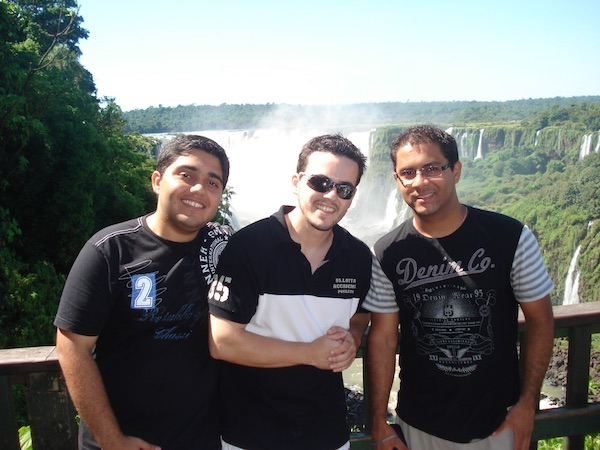
\includegraphics[width=\linewidth]{dso_sample}
  \caption{DSO-1 sample original image}\label{fig:dsooriginalimage}
\endminipage\hfill
\minipage{0.48\textwidth}
  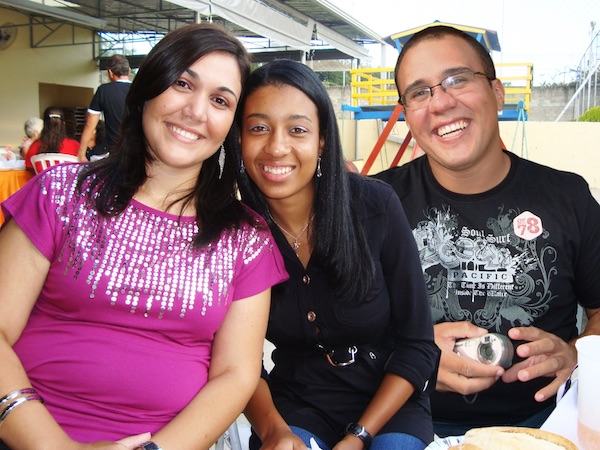
\includegraphics[width=\linewidth]{dso_sample_spliced}
  \caption{DSO-1 sample spliced image}\label{fig:dsosplicedimage}
\endminipage
\end{figure}

The forgeries were created by adding one or more individuals in a source image that already contained one or more people. When necessary, some post-processing operations were made (such as color and brightness adjustments) in order to increase photorealism.

\subsection{DSI-1}

The DSI-1 dataset is composed of 50 images with different resolutions (25 original and 25 doctored) downloaded from different websites in the Internet. Original images were downloaded from Flickr and doctored images were collected from different websites such as \emph{Worth 1000}, \emph{Benetton Group 2011}, \emph{Planet Hiltron}, etc.

\begin{figure}[!htb]
\minipage{0.46\textwidth}
  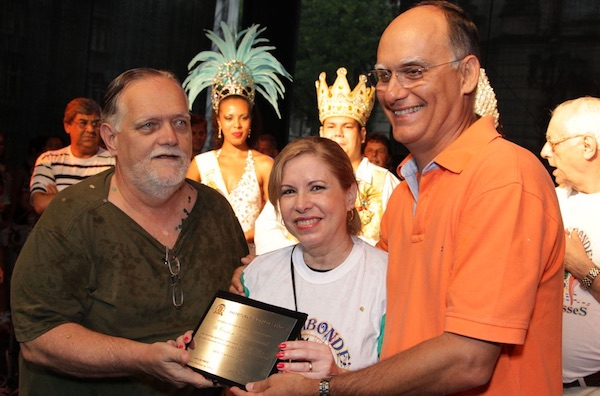
\includegraphics[width=\linewidth]{dsi_sample_normal}
  \caption{DSI-1 sample original image}\label{fig:dsioriginalimage}
\endminipage\hfill
\minipage{0.50\textwidth}
  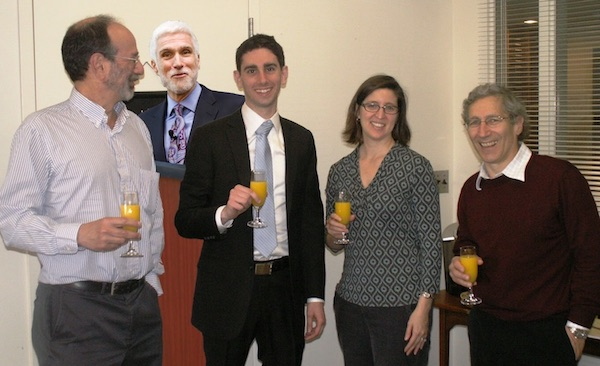
\includegraphics[width=\linewidth]{dsi_sample_spliced}
  \caption{DSI-1 sample spliced image}\label{fig:dsisplicedimage}
\endminipage
\end{figure}

\subsection{ColorChecker}

The ColorChecker dataset is a collection of images for evaluating Color Constancy algorithms built as additional material to \cite{gehler2008bayesian}. It consists in 568 RGB colored images of different scenes, both indoor and outdoor taken under different illuminations. In each scene a Gretag MacBeth Color Checker Chart was placed such that it was illuminated by the main scene illuminant and thus its color could be retrieved. The data is available in Canon RAW format free of any correction.

\begin{figure}[h!]
  \centering
    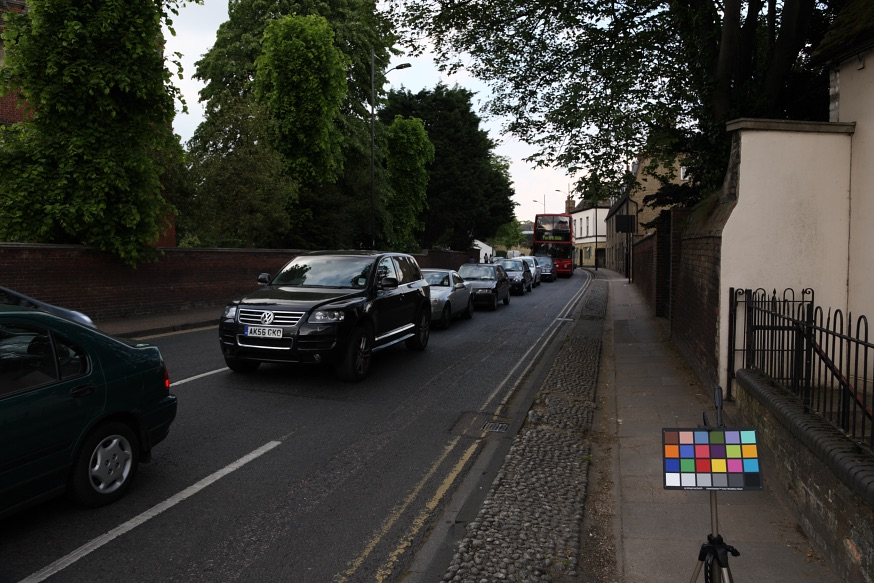
\includegraphics[width=0.65\textwidth]{colorchecker_sample}
    \caption{Example of an image of the ColorChecker dataset}
    \label{fig:colorcheckersample}
\end{figure}

\section{Face forgery detection module performance}

This section describes the experiments performed to evaluate the face forgery detection module. In these experiments, the DSO-1 and the DSI-1 datasets are used for evaluation.

After characterizing an image with a specific image descriptor, the next step consists of using an appropriate learning method.

the proposed method method focuses on using complementary information, the color descriptors, to describe the Illuminant Maps. Accordingly to Carvalho \emph{et al. }\cite{carvalho2016illuminant}, we selected the k-Nearest Neighbor (kNN) classifier instead of more powerful and computational intensive ones such as Support Vector Machines (SVM) due fact that, SVM and kNN, or even fusion of both learning methods, present very similar results, enforcing the choice for a simpler learning technique (kNN)\cite{carvalho2016illuminant}. The value of \emph{k} is set to 5. 

For all image descriptors, we have used the standard configuration proposed by Penatti \emph{et al.} \cite{penatti2012comparative}.

As described in Chapter 2, eight different kNN models are trained and used for the classification, considering all the possible combinations of the couples composed by a IMs transformed space (GGE e IIC)and a color descriptor (chosen from ACC, BIC, CCV and LCH).

\subsection{Color descriptors accuray}

Since the final classification output is given by majority voting of all the selected classifiers, the first round of experiments aimed at evaluating the accuracy of each image descriptors.

\begin{table}[h!]
\centering
\begin{tabular}{l c c c c c c} 
\hline \hline 
\textbf{Test case} & \textbf{Train} & \textbf{Test} & \textbf{ACC} & \textbf{BIC} & \textbf{CCV} & \textbf{LCH} \\ [0.5ex]
\hline
Test 1 & DSO-1 & DSO-1 &	0.75 & 0.75	& 0.72 & \textbf{0.78}\\
Test 2 & DSI-1 & DSI-1 &	0.78 & 0.79 & 0.77 & \textbf{0.82}\\
Test 3 &	DSO-1 &	DSI-1 &	0.56 & \textbf{0.57} & 0.53 & 0.53\\
Test 4 &	DSI-1 & DSO-1 & 0.58 & 0.55 & 0.51 & \textbf{0.59}\\ [1ex]
\hline
\end{tabular}
\caption{Accuracy for kNN technique using a single color descriptor. Experiments are performed using 10-fold cross-validation in test case number 1 and 2.}
\label{table:colordescriptorperformance}
\end{table}

Table \ref{table:colordescriptorperformance} shows the results of all tested combinations of train and test set. The classification results show that, generally, LCH color descriptor yielded the higher accurary, but there is not a descriptor that outperforms the others.

\subsection{Test cases}

After analyzing each single descriptor accuracy, we proceeded to evaluate the overall module using a combination of all of them, as described in Chapter 2. Since not all the color descriptors perform equally, a different weight is given at each classifier.

In the following experiments, the  method has been applied for classifying a face pair as fake or real using uniform (Table \ref{table:performancefacedet}) and non-uniform (Table \ref{table:performancefacedetnonun}) weights. Essentially, these experiments evaluate the forgery detection performances.

For each test case in the suite it is reported:
\begin{enumerate}
\item The training dataset (\textbf{\emph{Train}});
\item The evaluation dataset (\textbf{\emph{Test}});
\item The classification accuracy score (\textbf{\emph{Accuracy}});
\item The area under the R\emph{eceiver Operator Characteristic (ROC)} curve (\textbf{\emph{AUC}})
\item The accuracy score expressed through the $F_1$ score (also known as \textbf{\emph{F-Score}})
\end{enumerate}

Accordingly with Jeni \emph{et al.} \cite{jeni2013facing}, when dealing with AUC score to measure the performance of classifier, one of the major drawbacks relies on the fact that an increasing of AUC doesn't really mean a better classifier, but it could be just the side-effect of too many negative examples used in training.

Therefore, another classification accuracy score is also provided, the \emph{F-Score}. Given $TP$, $FP$ and $FN$ the true positives, false positives and false negatives values. 

Let the classification \emph{precision} score given by

$$
precision = \frac{TP}{TP + FP}
$$

where $TP$ and $FP$ are true positives and false positives respectively.

The \emph{recall} value is defined as
$$
recall = \frac{TP}{TP + FN}
$$
where $FN$ stands for false negatives. The $F_{\beta}$ score is defined as the harmonic mean of precision and recall values:

\begin{equation}
F_{\beta} = (1 + \beta^2) * \frac{precision * recall}{(\beta^2 * precision) + recall}
\end{equation}

where $\beta$ states for the relative importance given to precision comparing to recall. In our experiments, we considered $\beta = 1$ (i.e. the $F_1$ score), so:
\begin{equation}
F_{1} = 2 * \frac{precision * recall}{precision + recall}  = \cdots = \frac{2 * TP}{2 * TP + FP + FN}
\end{equation}

In order to proceed with the comparison between using uniform and non-uniform weights for classifiers, we have to determine the most appropriate weight values for each descriptor. The weights have been found with an exhaustive search by evaluating the performance of the currently analyzed weights combination over the DSO-1 dataset with a 10-fold cross-validation protocol. 

To reduce the computational cost, we limited the range of values to be explored for each classifier basing on the results reached for each single descriptor, presented in Table \ref{table:colordescriptorperformance}, giving more importance to LCH descriptor.

Experimental results are collected in Table \ref{table:performancefacedet}, for the uniform weights case, and in Table \ref{table:performancefacedetnonun}, for non-uniform case. 

\begin{table}[h!]
\centering
\begin{tabular}{l c c c c c} 
\hline \hline 
\textbf{Test case} & \textbf{Train} & \textbf{Test} & \textbf{ACC} & \textbf{AUC} &\textbf{ F-Score} \\ [0.5ex]
\hline
Test 1 & DSO-1 & DSO-1 &	0.82 & 0.88	& 0.77\\
Test 2 & DSI-1 & DSI-1 &	0.87 & 0.92 & 0.87\\
Test 3 &	DSO-1 &	DSI-1 &	0.58 & 0.58 & 0.62\\
Test 4 &	DSI-1 & DSO-1 & 0.62 & 0.59 & 0.53\\ [1ex]
\hline
\end{tabular}
\caption{Performance of face forgery detection module over paired faces using uniform weights.}
\label{table:performancefacedet}
\end{table}

\begin{table}[h!]
\centering
\begin{tabular}{l c c c c c} 
\hline \hline 
\textbf{Test case} & \textbf{Train} & \textbf{Test} & \textbf{ACC} & \textbf{AUC} &\textbf{ F-Score} \\ [0.5ex]
\hline
Test 1 & DSO-1 & DSO-1 &	0.84 & 0.90	& 0.78\\
Test 2 & DSI-1 & DSI-1 &	0.89 & 0.92 & 0.89\\
Test 3 &	DSO-1 &	DSI-1 &	0.59 & 0.58 & 0.64\\
Test 4 &	DSI-1 & DSO-1 & 0.63 & 0.60 & 0.54\\ [1ex]
\hline
\end{tabular}
\caption{Performance of face forgery detection module over paired faces using non-uniform weights.}
\label{table:performancefacedetnonun}
\end{table}

Resulting accuracy scores are obtained as average over 5 consecutive runs of the algorithm. For a better visualization, Figure \ref{fig:compareknnweights} depicts a direct comparison between the accuracy of both results as a bar graph.

\begin{figure}[h!]
  \centering
    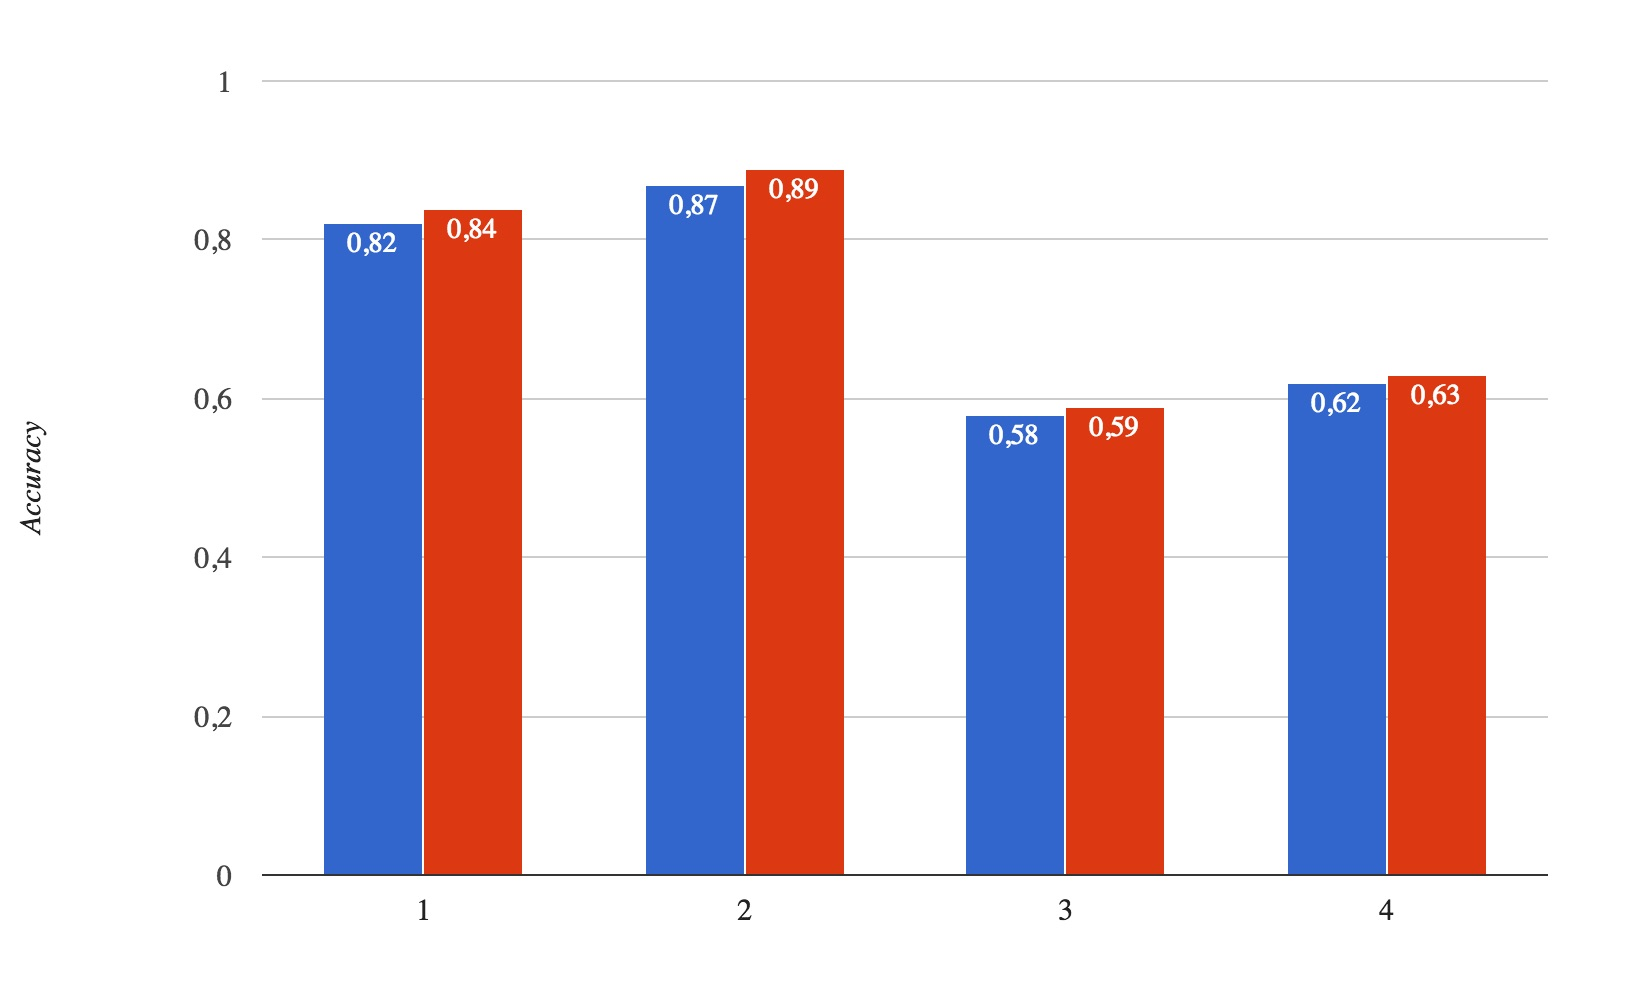
\includegraphics[width=0.9\textwidth]{compareknnweights}
    \caption{Classification accuracies comparison between using uniform and non uniform weights for kNN classifiers over the considered 4 test cases of Table \ref{table:performancefacedet}. The blue bins depict the reached accuracies using uniform weights, reds are for non-uniform case.}
    \label{fig:compareknnweights}
\end{figure}

These results show that, although we can notice a slight performance improvement in all test cases, the use of non-uniform weights do not affect much on the final classification results.

In the following subsections are described the experimental results for each analyzed test case using non-uniform weights. We show results using classical \emph{Receiver Operator Characteristic (ROC)} \cite{fawcett2006introduction} and Precision-Recall curves\cite{Davis:2006:RPR:1143844.1143874}. 

\subsubsection{Performance on DSO-1 dataset}

In this experiment, we applied the proposed method for classifying a face pair as fake or real considering only the DSO-1 dataset. We reached an average accuracy of 84\%.

\begin{figure}[!htb]
\minipage{0.42\textwidth}
  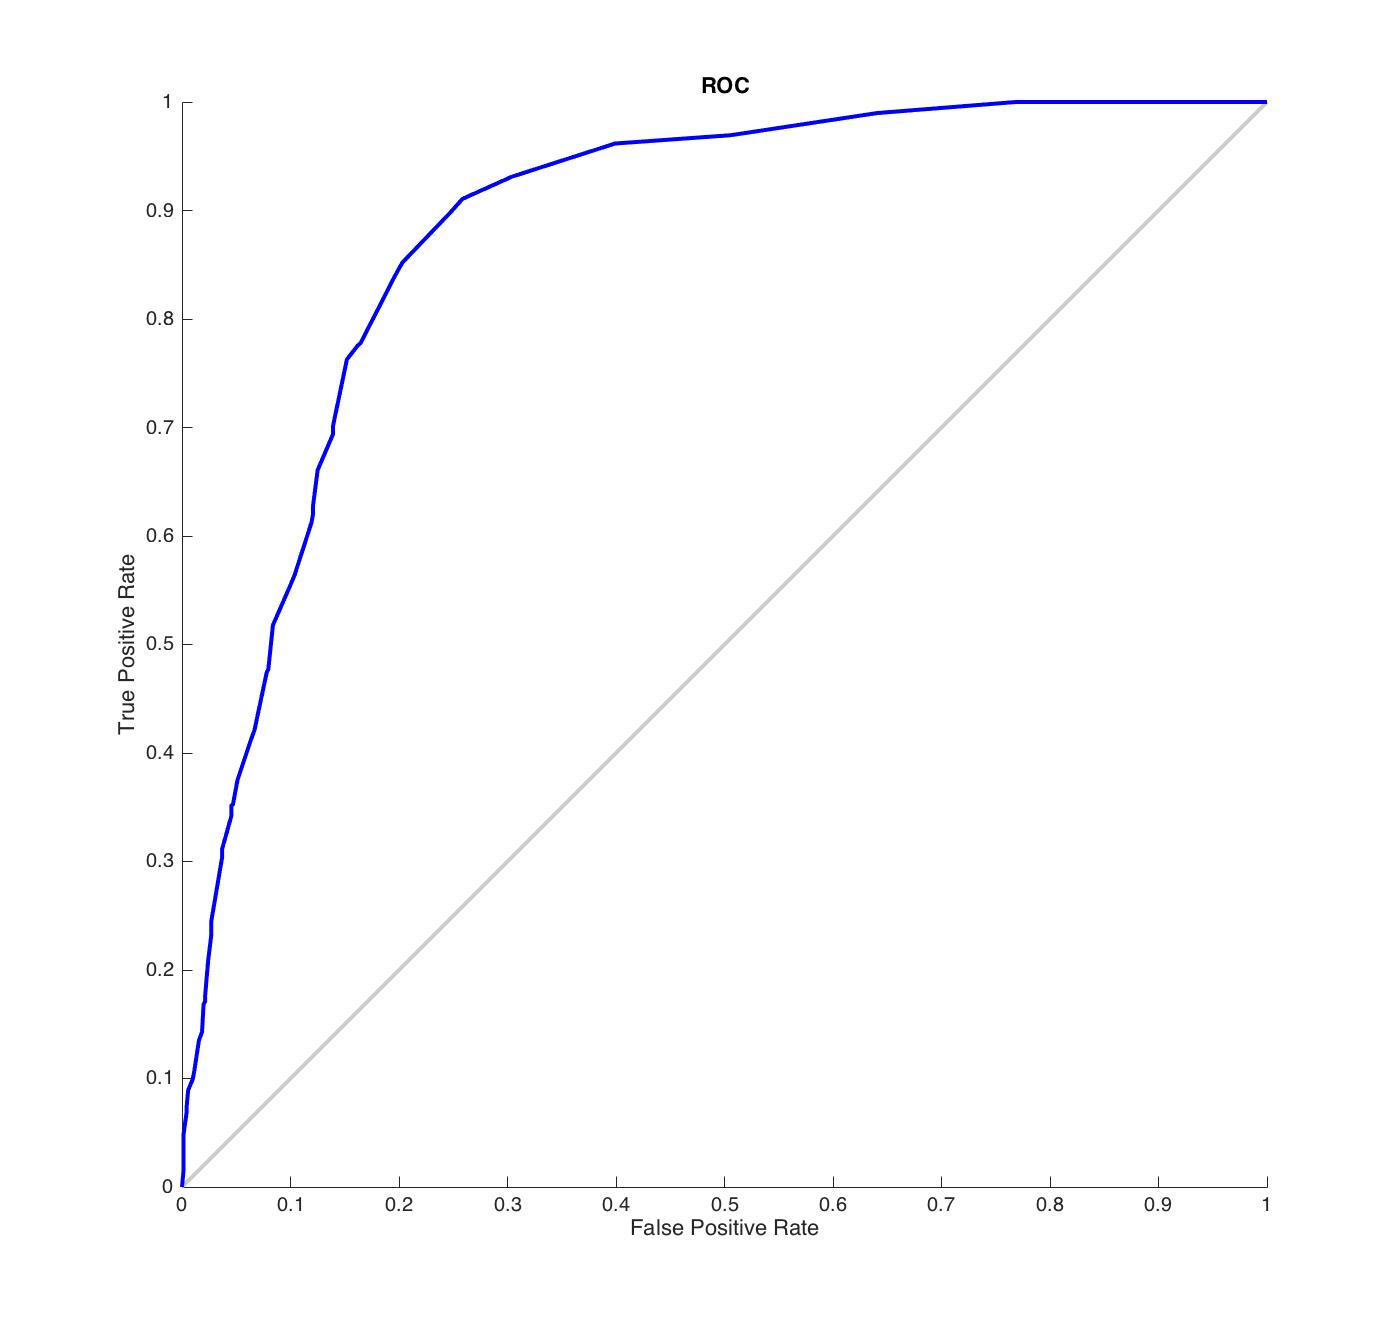
\includegraphics[width=\linewidth]{train_dso_crossvalidation}
\endminipage\hfill
\minipage{0.53\textwidth}
  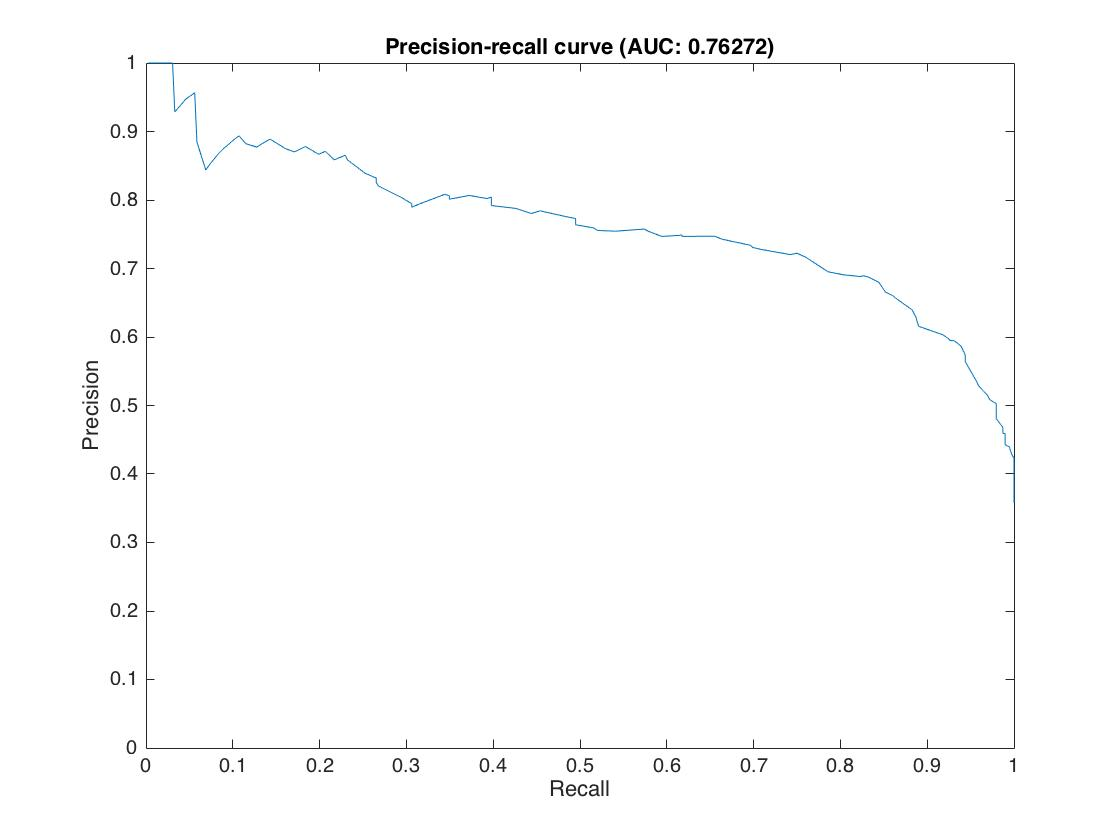
\includegraphics[width=\linewidth]{train_dso_crossvalidation_prec_rec}
\endminipage
\caption{ROC curve and Precision-Recall curve for DSO-1 cross-validation classification of paired faces.}\label{fig:regiondetnormal}
\end{figure}

\subsubsection{Performance on DSI-1 dataset}

\begin{figure}[!htb]
\minipage{0.42\textwidth}
  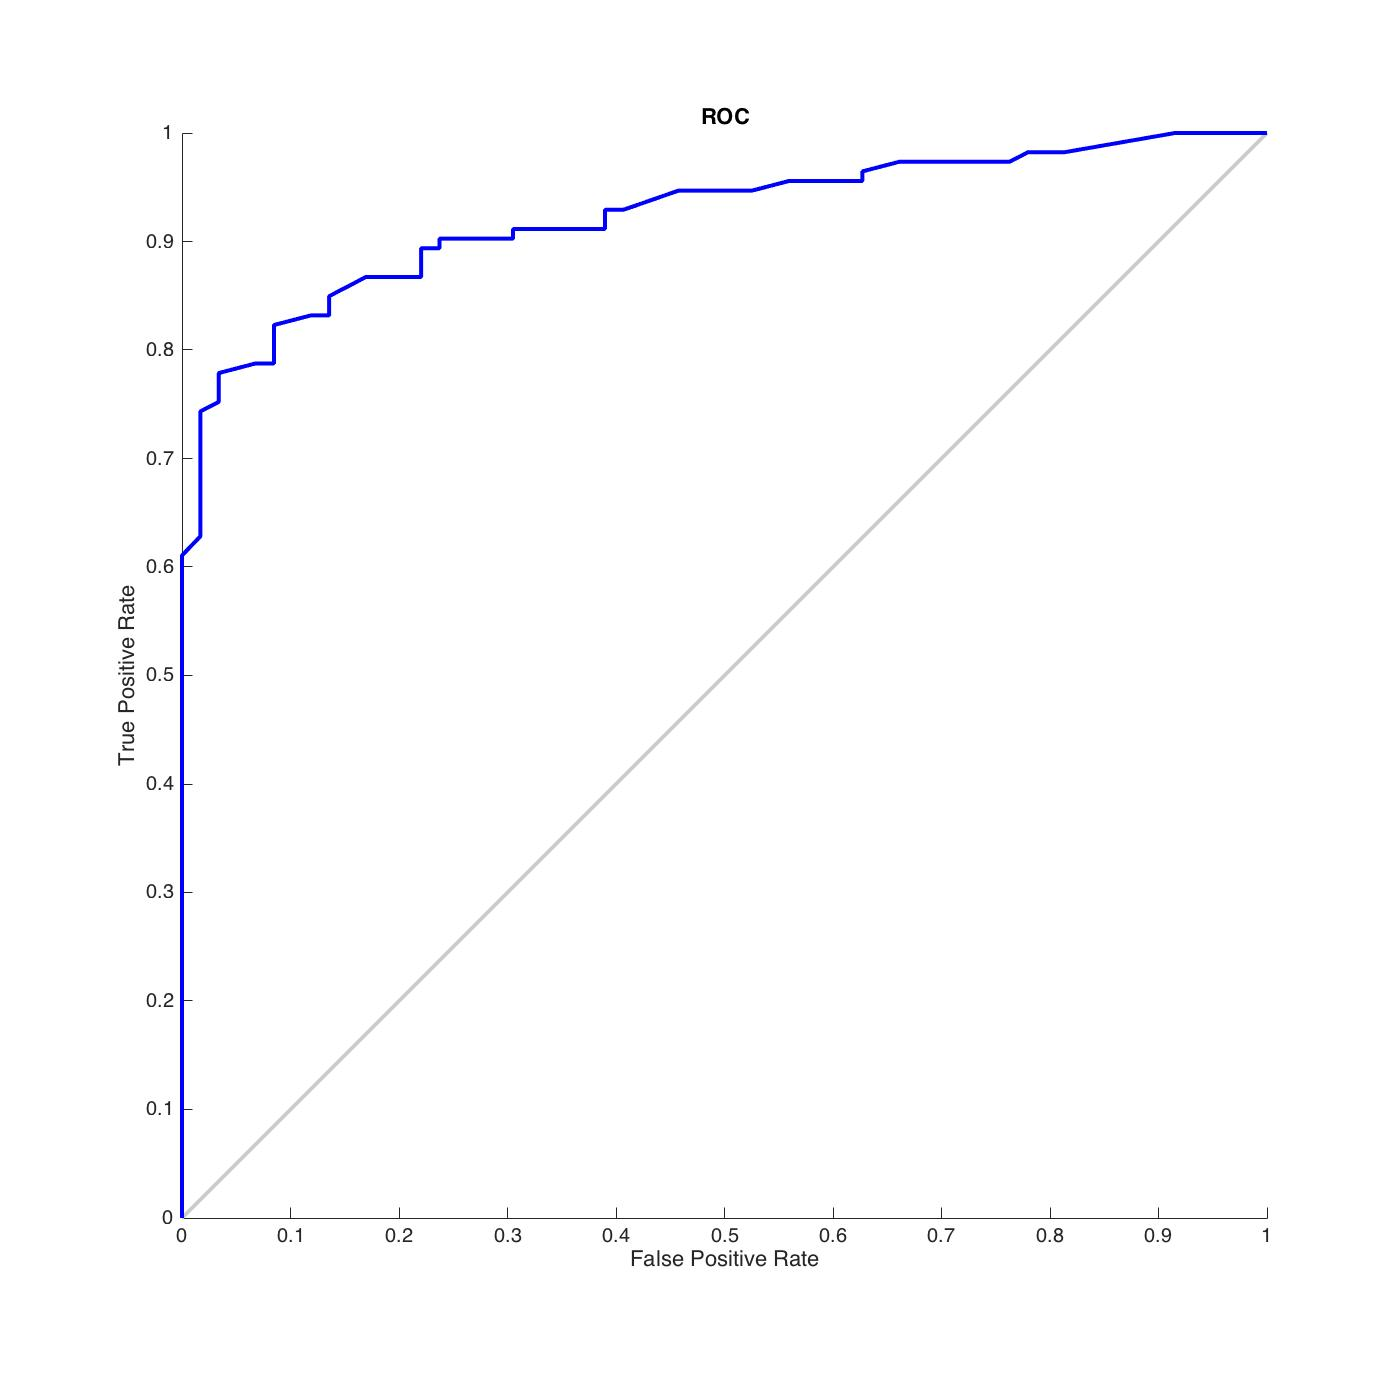
\includegraphics[width=\linewidth]{train_dsi_crossvalidation}
\endminipage\hfill
\minipage{0.53\textwidth}
  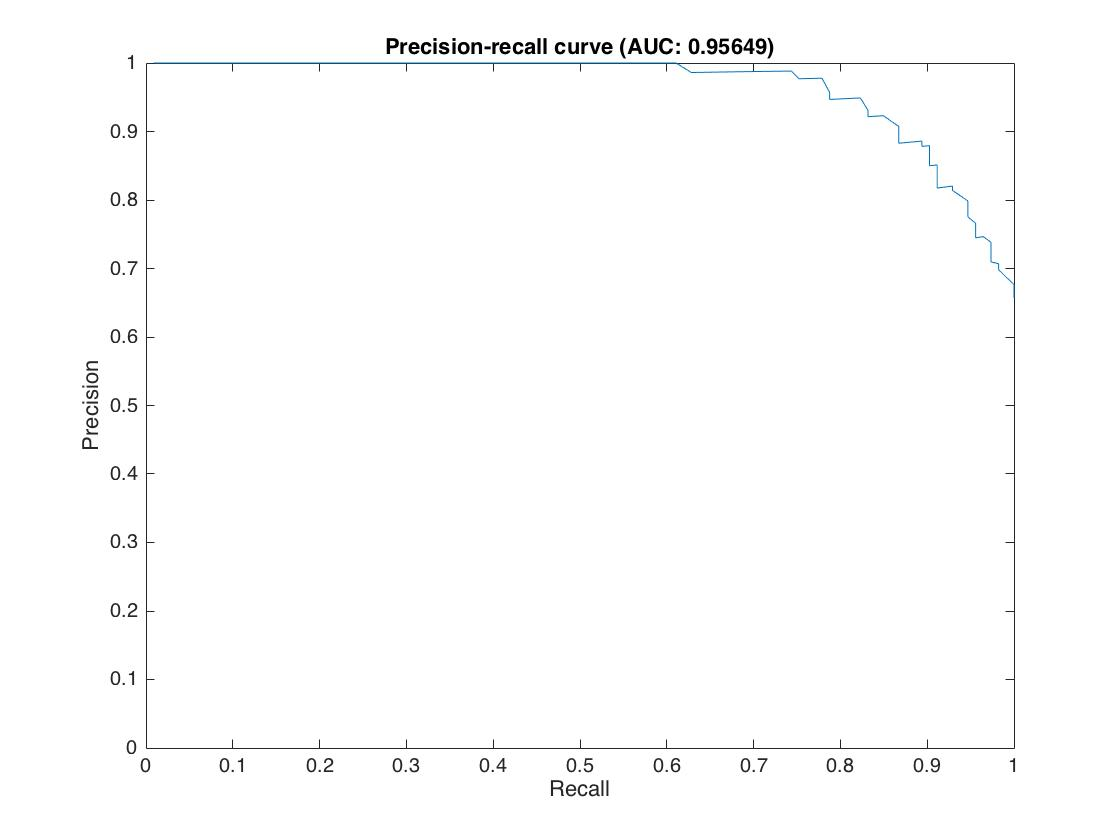
\includegraphics[width=\linewidth]{train_dsi_crossvalidation_prec_rec}
\endminipage
\caption{ROC curve and Precision-Recall curve for DSI-1 cross-validation classification of paired faces.}\label{fig:regiondetnormal}
\end{figure}

\subsubsection{Cross dataset performance on DSO-1}

\begin{figure}[!htb]
\minipage{0.42\textwidth}
  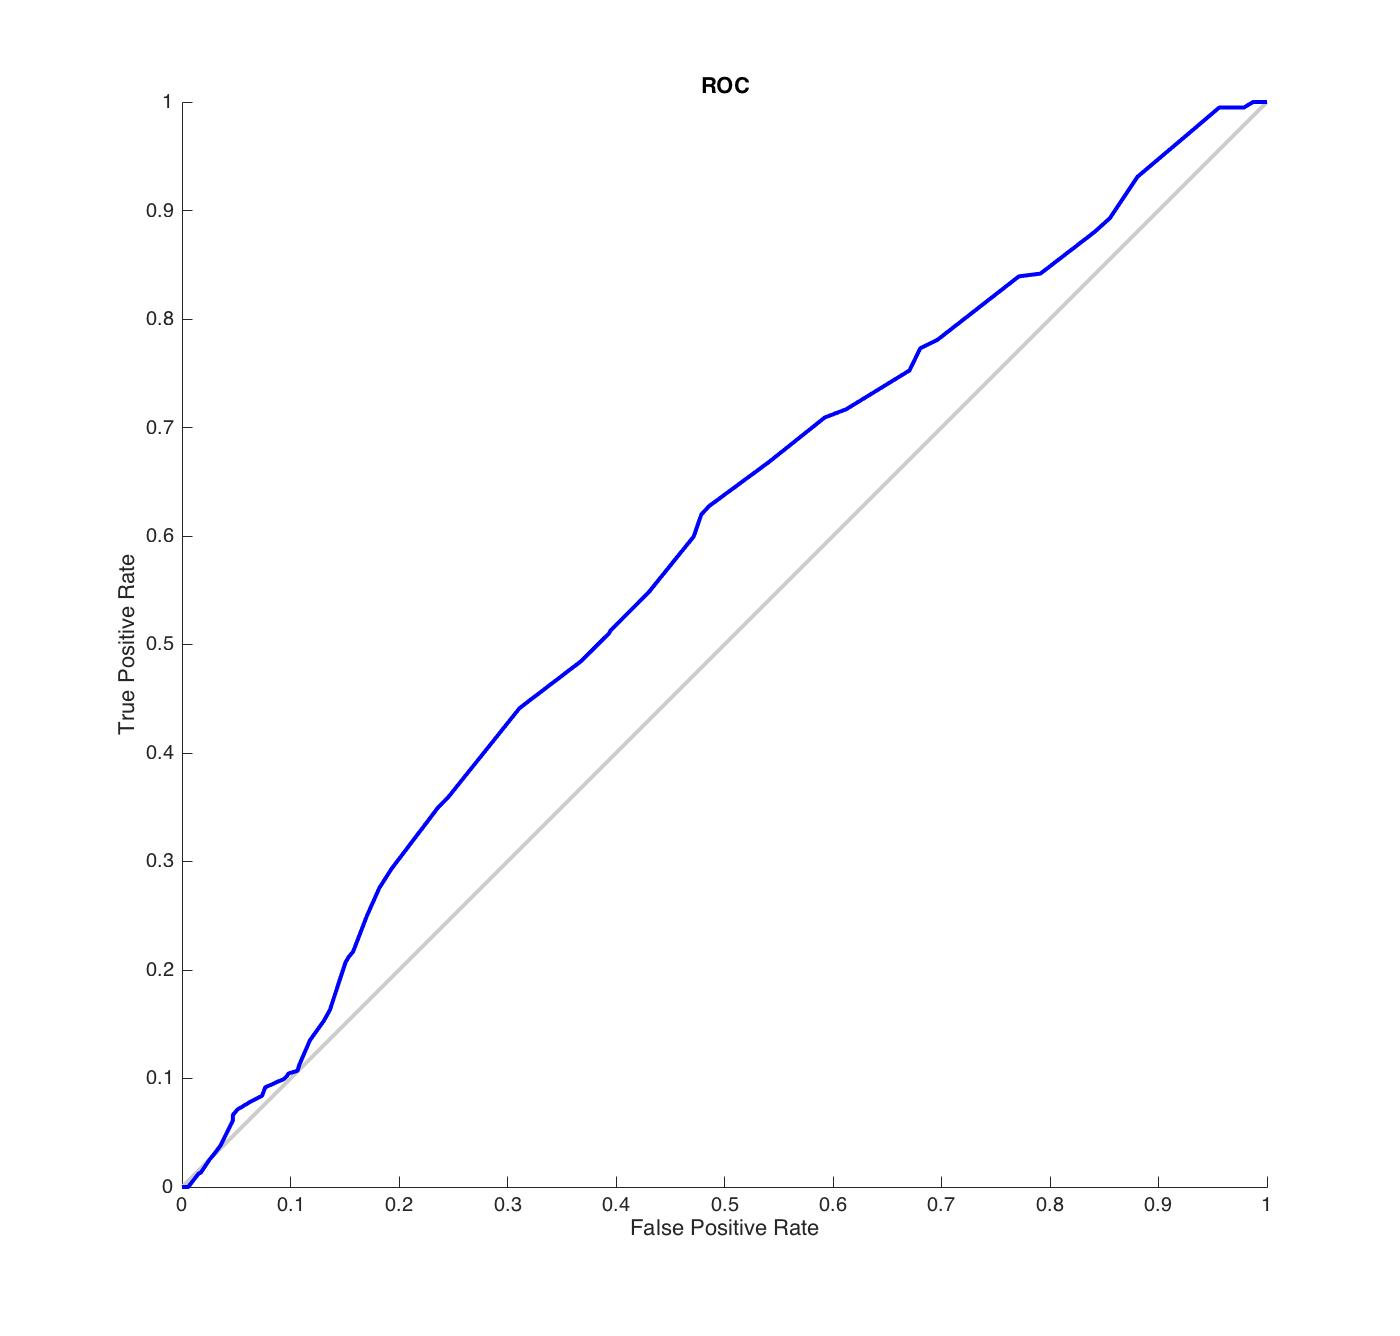
\includegraphics[width=\linewidth]{train_dsi_test_dso}
\endminipage\hfill
\minipage{0.53\textwidth}
  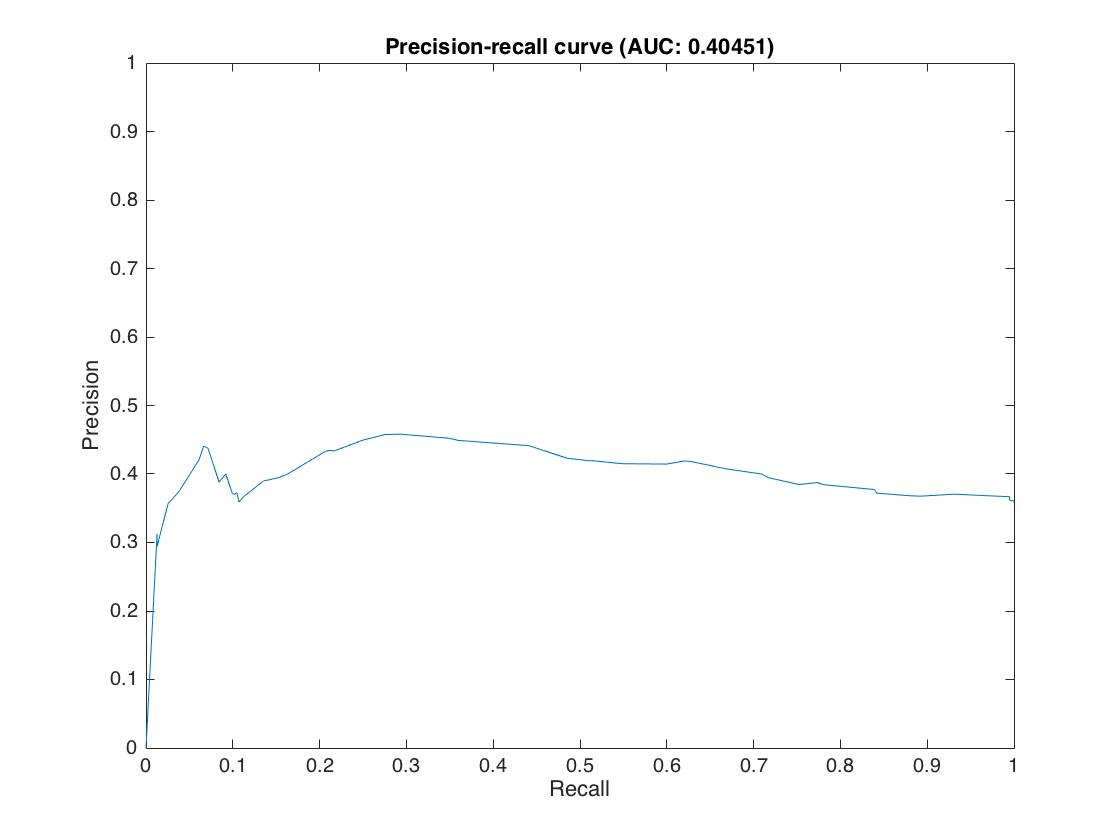
\includegraphics[width=\linewidth]{train_dsi_test_dso_prec_rec}
\endminipage
\caption{ROC curve and Precision-Recall curve for DSO-1 paired faces classification using trained data on DSI-1.}\label{fig:regiondetnormal}
\end{figure}

\subsubsection{Cross dataset performance on DSI-1}

\begin{figure}[!htb]
\minipage{0.42\textwidth}
  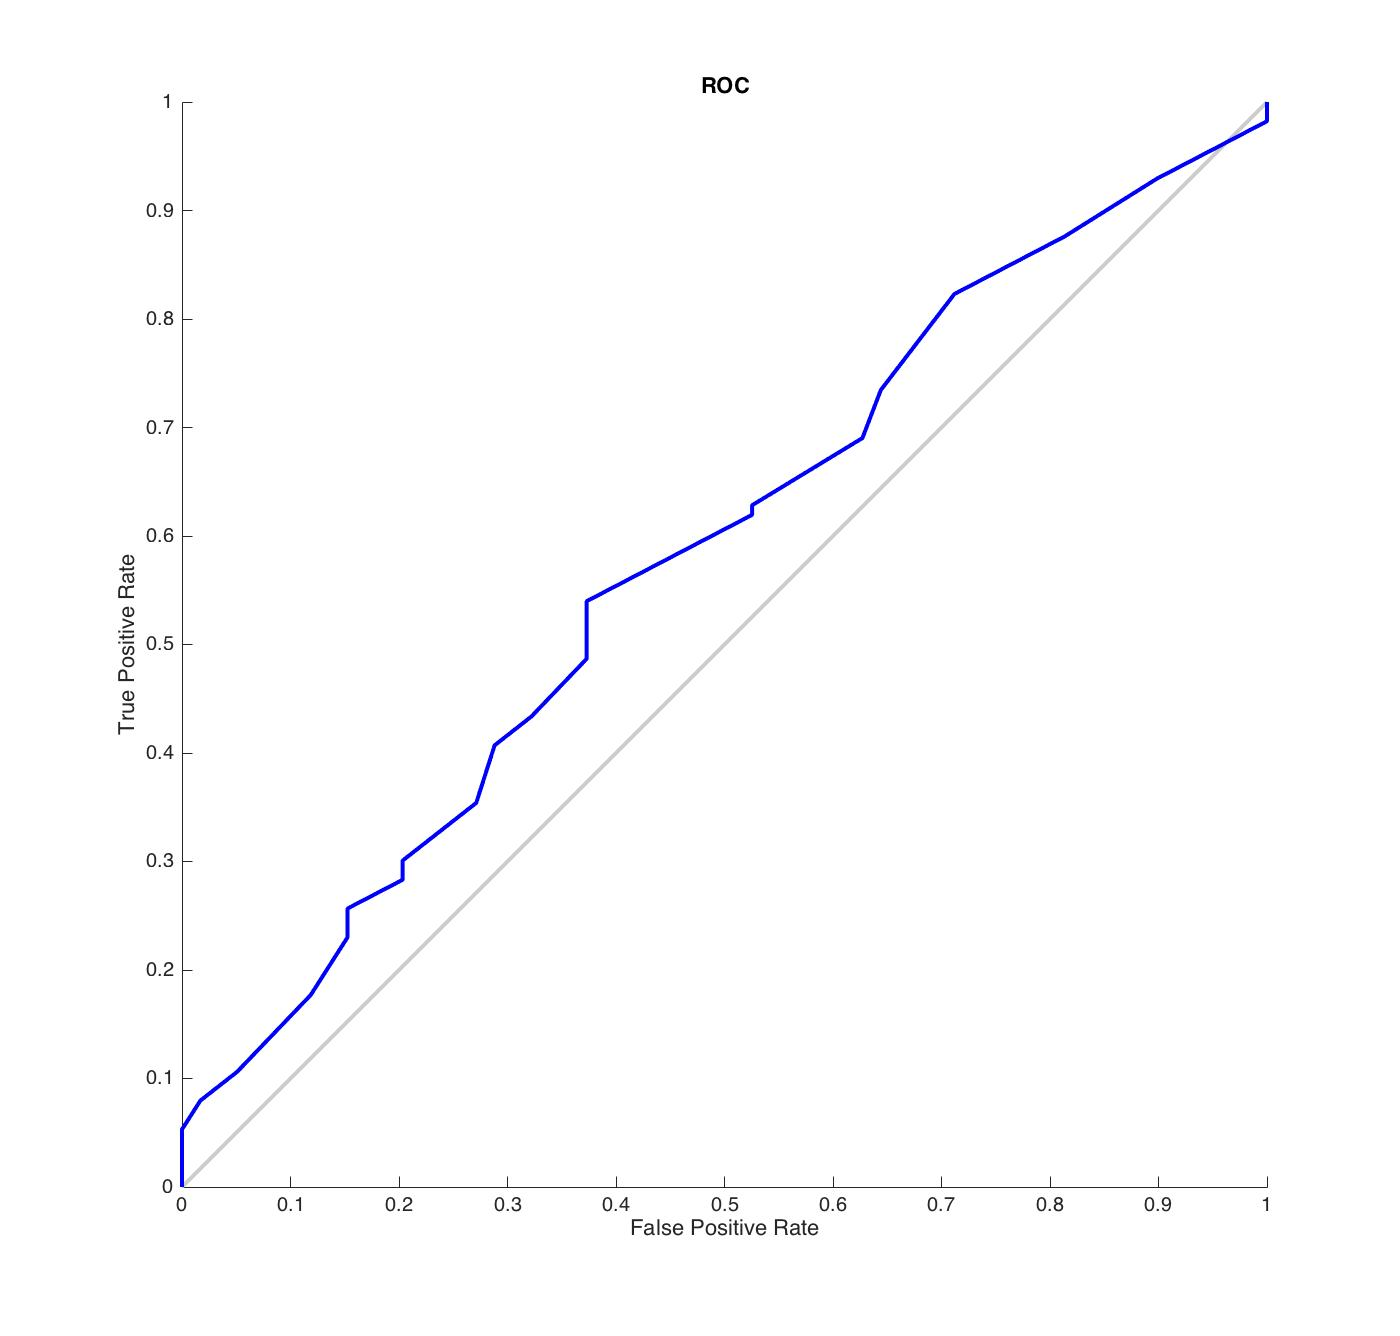
\includegraphics[width=\linewidth]{train_dso_test_dsi}
\endminipage\hfill
\minipage{0.53\textwidth}
  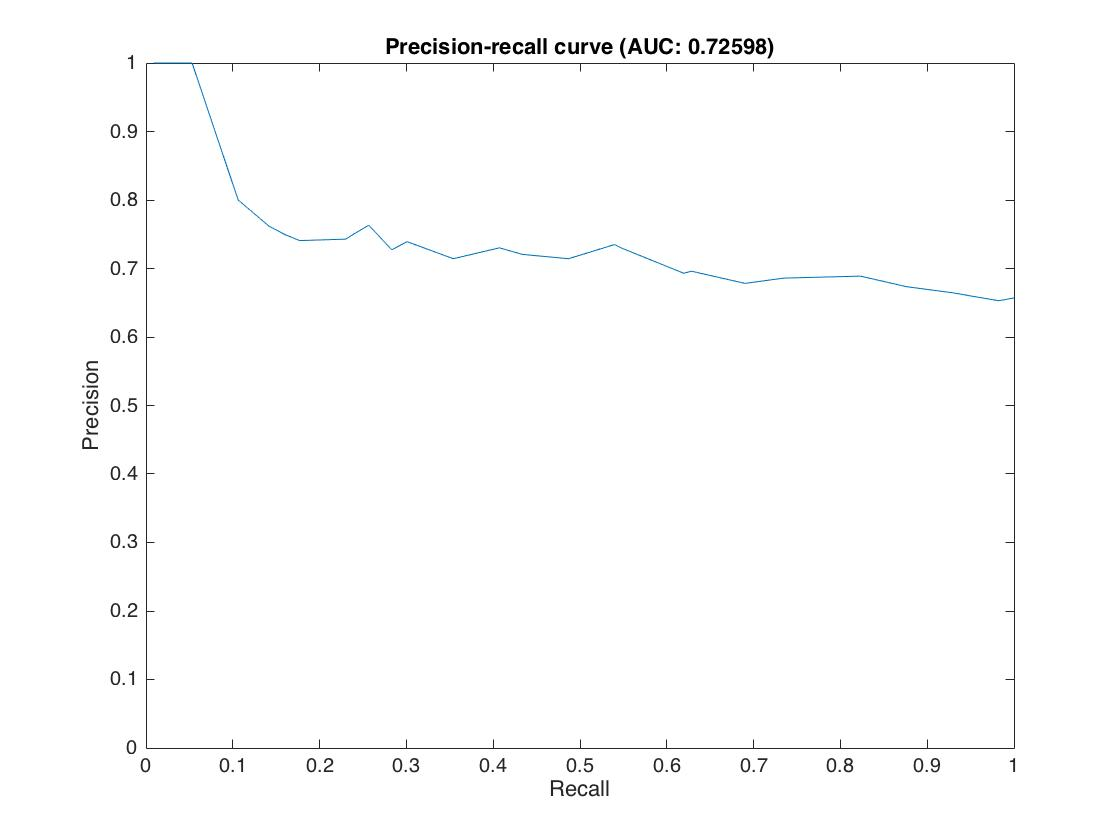
\includegraphics[width=\linewidth]{train_dso_test_dsi_prec_rec}
\endminipage
\caption{ROC curve and Precision-Recall curve for DSI-1 paired faces classification using trained data on DSO-1.}\label{fig:regiondetnormal}
\end{figure}


\subsubsection{Forgery detection performance}

In the following experiments, we used the proposed module to detect the face with the highest probability of being the fake face in an image tagged as fake by the classifier. 

In this round of experiments, we assume that the input image $I$ has already been classified as fake by the classifier (i.e. at least one couple of faces has been classified as fake). 

We performed this kind of experiments using both DSO-1 and DSI-1 datasets. For each test in the suite it is reported:
\begin{itemize}
\item The training dataset (\textbf{Train})
\item The evaluation dataset (\textbf{Test})
\item The total number of faces detected in the images (\textbf{Faces})
\item The true positive rate (\textbf{TPR})
\item The classification accuracy (\textbf{ACC})
\item The classification precision (\textbf{PREC})
\item The classification recall (\textbf{REC})
\item The $F_1$ score (\textbf{F-Score})
\end{itemize}

Experimental results are collected in Table \ref{forgerydetections}.

\begin{table}[h!]
\centering
\begin{tabular}{l c c c c c c c} 
\hline \hline 
\textbf{N.} & \textbf{Train} & \textbf{Test} & \textbf{Faces} & \textbf{PREC} & \textbf{REC} & \textbf{ACC} & \textbf{F-Score} \\ [0.5ex]
\hline
1 & DSO-1 & DSO-1 &	540 & 0.58 & 0.89 & 0.81	& 0.64\\
2 & DSI-1 & DSI-1 &	133 & 0.56 & 0.95 & 0.75 & 0.66\\
3 &	DSO-1 & DSI-1 & 540 & 0.31 & 0.18 & 0.63 & 0.25\\ 
4 &	DSI-1 &	DSO-1 &	130 & 0.34 & 0.43 & 0.67 & 0.37\\[1ex]

\hline
\end{tabular}
\caption{Performance of face forgery detection module over single faces using non-uniform weights.}
\label{table:forgerydetections}
\end{table}


\section{Regions forgery detection module performance}

This section describes the experiments performed to evaluate the regions forgery detection module.

\subsection{Creating the training set}

Since the method is based on the classification of entire bands of images, in order to train the SVM classifiers were created two different training set with specific requirements:
\begin{itemize}
\item Each image must have only one spliced band (either horizontal or vertical)
\item The spliced region of the image must consist only int the whole band
\item The spliced region position in the image must be chosen randomly
\end{itemize}

Each image in the dataset must be shipped with its spliced band position as groundtruth (for performance evaluation).

For the two new training set, the DSO-1 and ColorChecker datasets were used respectively as source. Each training set is splitted into two subset containing only vertical or horizontal spliced bands.

\begin{algorithm}[!h]
\begin{algorithmic}[1]
\State Let $d \in \{vertical, horizontal\}$ a direction
\State Let $S$ be the band size
\For {each image $i \in SourceDataset$}
\State Select another image $j$ randomly from the same set with $i \neq j$
\State Resize $j$ to fit $i$
\State Select a band $b$ of direction $d$ randomly from $j$
\State Put $b$ in $i$ at the same original position
\State Save $i$ as image
\EndFor
\end{algorithmic}\caption{Spliced dataset creation algorithm}\label{alg:spliceddatasetcreation}
\end{algorithm}

The pseudocode used for generating the spliced datasets is proposed in Algorithm \ref{alg:spliceddatasetcreation}. That procedure is repeated for both DSO-1 and ColorChecher as $SourceDataset$ and for each direction. We called \emph{SplicedDSO} the dataset generated from DSO-1, \emph{SplicedCC} the one from ColorCherer. Both have 200 images vertically and horizontally spliced.

\begin{figure}[!htb]
\minipage{0.48\textwidth}
  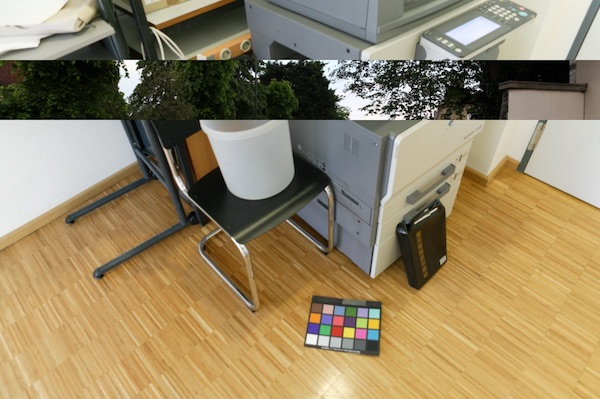
\includegraphics[width=\linewidth]{splicedcchor}
\endminipage\hfill
\minipage{0.48\textwidth}
  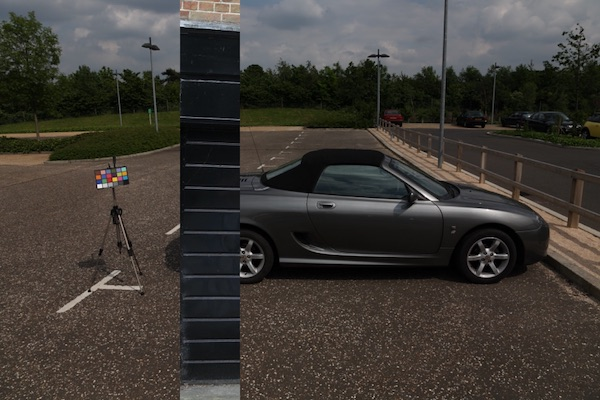
\includegraphics[width=\linewidth]{splicedccver}
\endminipage
\caption{Example images from the generated \emph{SplicedCC} dataset. Left with horizontal spliced band, right with vertical.}\label{fig:splicedccsamples}
\end{figure}

\begin{figure}[!htb]
\minipage{0.48\textwidth}
  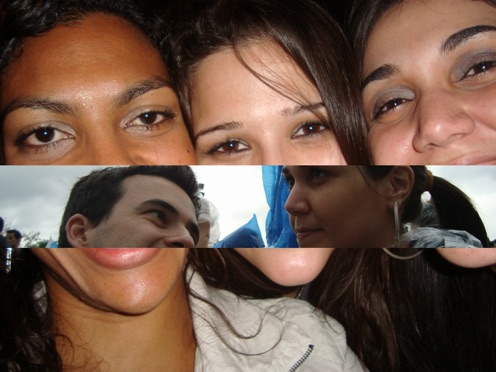
\includegraphics[width=\linewidth]{spliceddsohor}
\endminipage\hfill
\minipage{0.48\textwidth}
  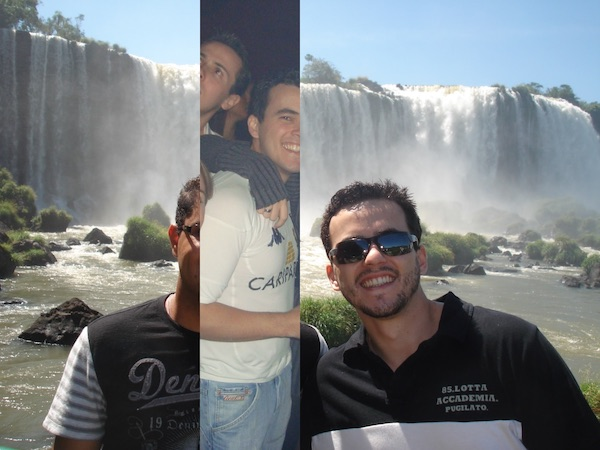
\includegraphics[width=\linewidth]{spliceddsover}
\endminipage
\caption{Example images from the generated \emph{SplicedDSO} dataset. Left with horizontal spliced band, right with vertical.}\label{fig:spliceddsosamples}
\end{figure}

Figure \ref{splicedccsamples} and \ref{fig:spliceddsosamples} show some example of generated images from both dataset. 

\subsection{Evaluating module performance}

The proposed method output consists in a\emph{ detection map} related to the analyzed image. In order to evaluate the performance of the module, we consider the single pixels classification accuracies. The evaluation dataset for all the experiments is the original DSO-1 dataset (considering only the spliced images).

Given a set of $m$ images as validation test, for each test in the suite:
\begin{enumerate}
\item Let $I$ the $i$-th analyzed image, a detection map $D_i$ is computed with our module.
\item Let $\mathcal{P}_i$ the subset of pixels in the image corresponding to the spliced region and let $\mathcal{S}_{\mathcal{P}_i}$ their corresponding values extracted from $D$. Finally, let $N_i$ the subset of pixels in the image corresponding to its original part and let $\mathcal{S}_{\mathcal{N}_i}$ their corresponding values extracted from $D_i$.
\item Step 1 and 2 are repeated for each image in the validation step, joining the resulting sets of scores:
$$
\mathcal{S}_{\mathcal{P}} = \cup_{i = 1}^{m} \mathcal{S}_{\mathcal{P}_i}
$$
$$
\mathcal{S}_{\mathcal{N}} = \cup_{i = 1}^{m} \mathcal{S}_{\mathcal{N}_i}
$$
\end{enumerate}

The two resulting sets of scores, $\mathcal{S}_{\mathcal{P}}$ and $\mathcal{S}_{\mathcal{N}}$ are used for evaluating overall performances.

The size of the evaluation dataset is limited to 25 image due the  required computational time. In the classification stage, we used an SVM classifier with an RBF kernel, and classical grid search for adjusting parameters in training samples \cite{bishop2007pattern}.

Experimental results are collected in Table \ref{table:performanceregionaldet}.

\begin{table}[h!]
\centering
\begin{tabular}{l c c c c c} 
\hline \hline 
\textbf{Test case} & \textbf{Train} & \textbf{RC} & \textbf{ACC} & \textbf{AUC} &\textbf{ F-Score} \\ [0.5ex]
\hline
Test 1 & - & Median & 0.49 & 0.32 & 0.25\\
Test 2 & - & Global & 0.52 & 0.40 & 0.27\\
Test 3 & SplicedCC & Median & 0.54 & 0.53 & 0.26\\
Test 4 & SplicedCC & Global & 0.57 & 0.57 & 0.31\\
Test 5 &	 SplicedDSO & Median & 0.53 & 0.50 & 0.27\\
Test 6 &	 SplicedDSO & Global & 0.61 & 0.63 & 0.33\\ [1ex]
\hline
\end{tabular}
\caption{Performance of region forgery detection module.}
\label{table:performanceregionaldet}
\end{table}

\subsection{Test cases}

\subsubsection{Performance without training}

\begin{figure}[!htb]
\minipage{0.42\textwidth}
  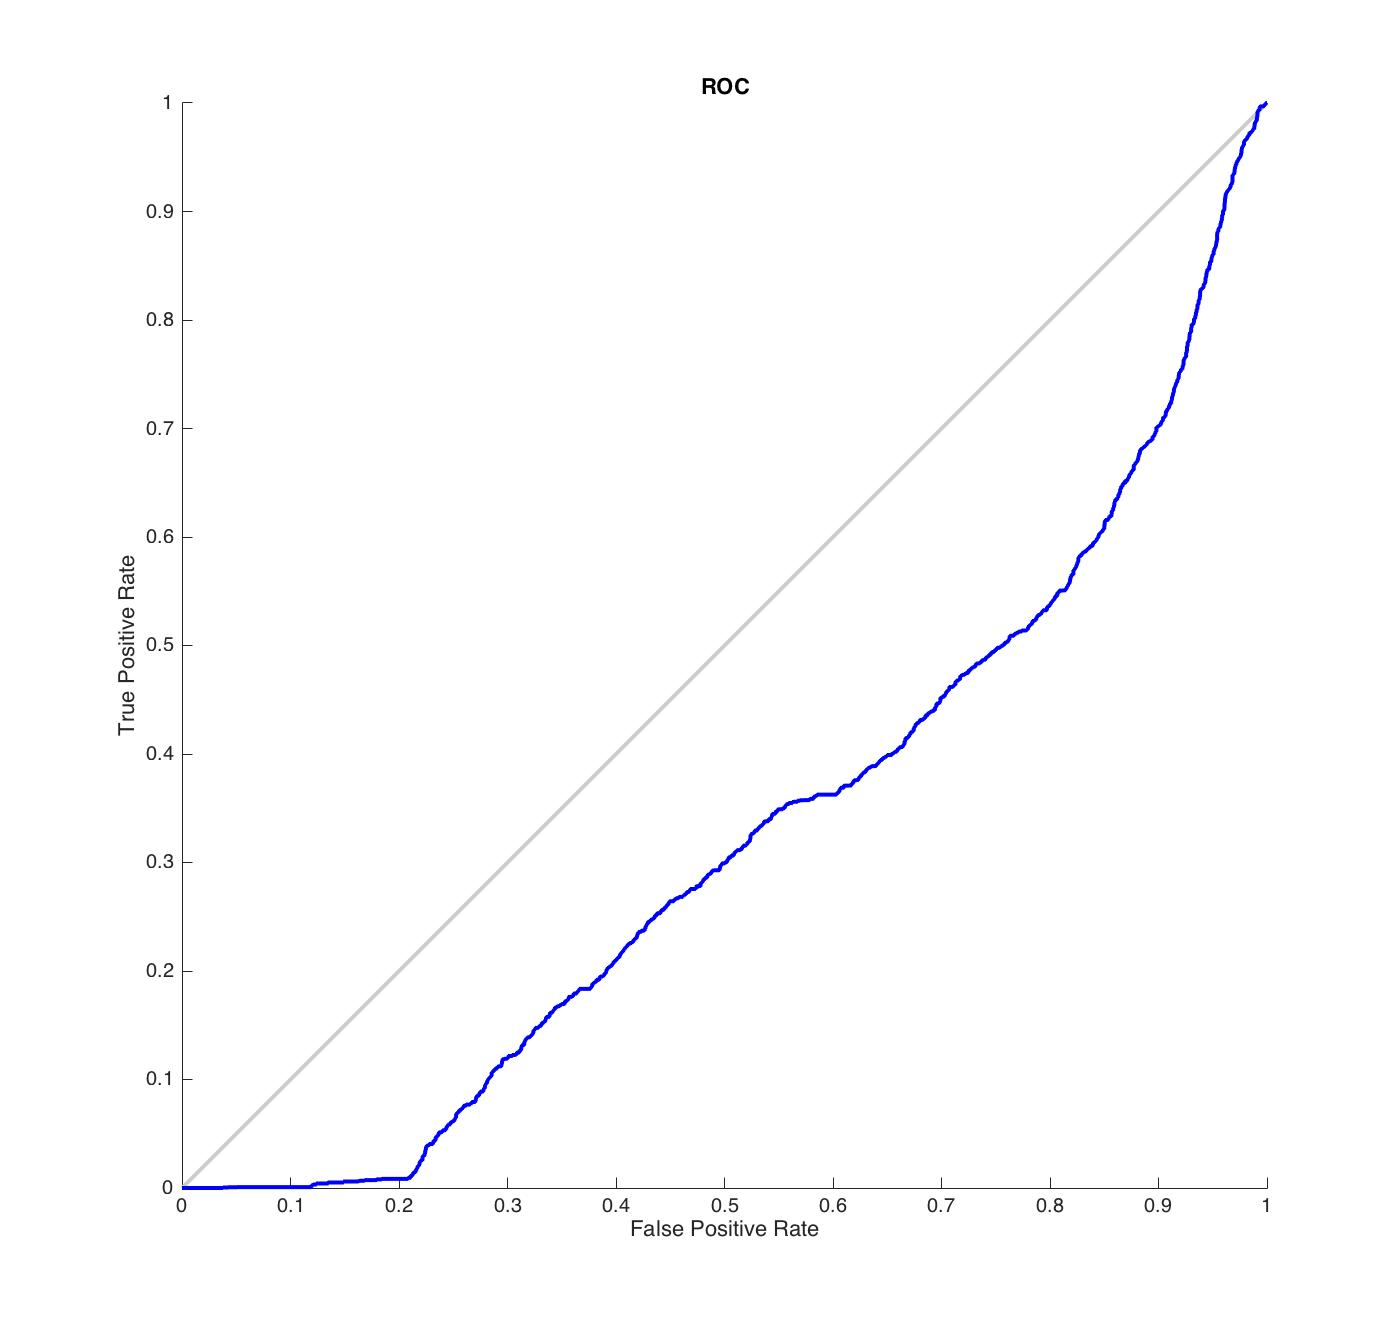
\includegraphics[width=\linewidth]{train_cc/roc_normal}
\endminipage\hfill
\minipage{0.53\textwidth}
  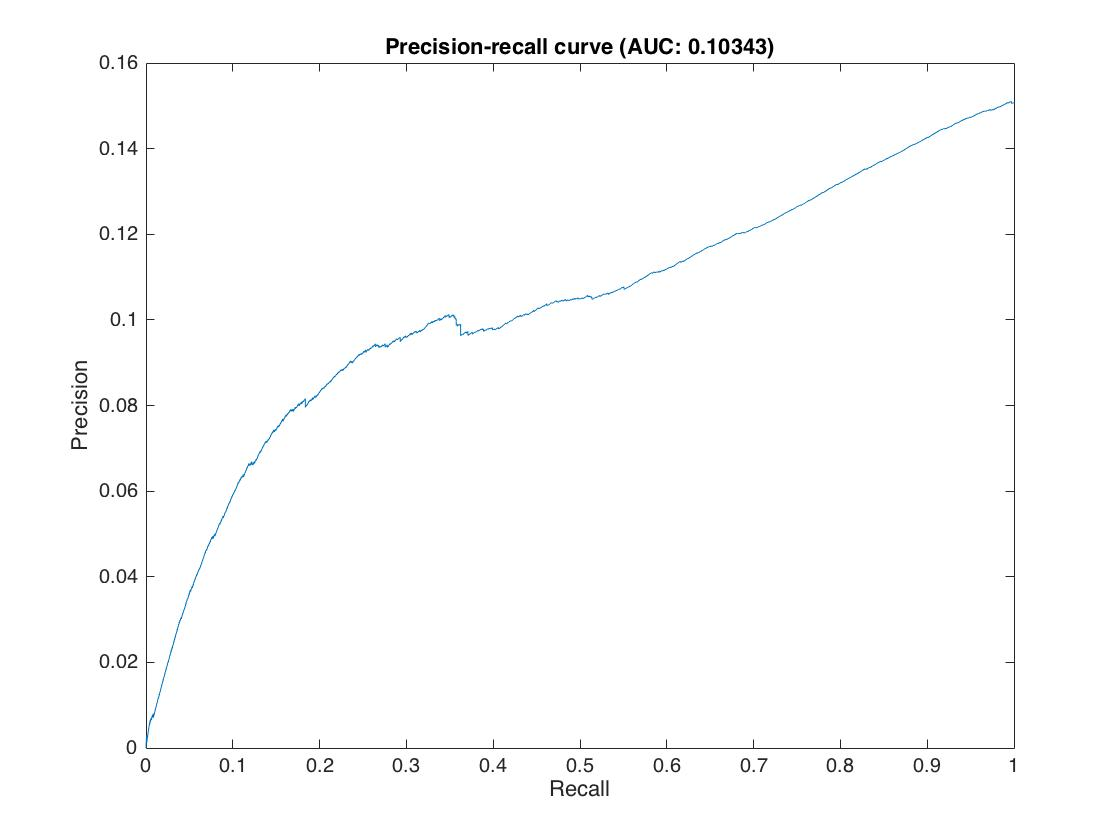
\includegraphics[width=\linewidth]{train_cc/prec_rec_normal}
\endminipage
\caption{ROC curve and Precision-Recall curve for classification without training, using the median reference value.}\label{fig:regiondetnormal}
\end{figure}

\begin{figure}[!htb]
\minipage{0.42\textwidth}
  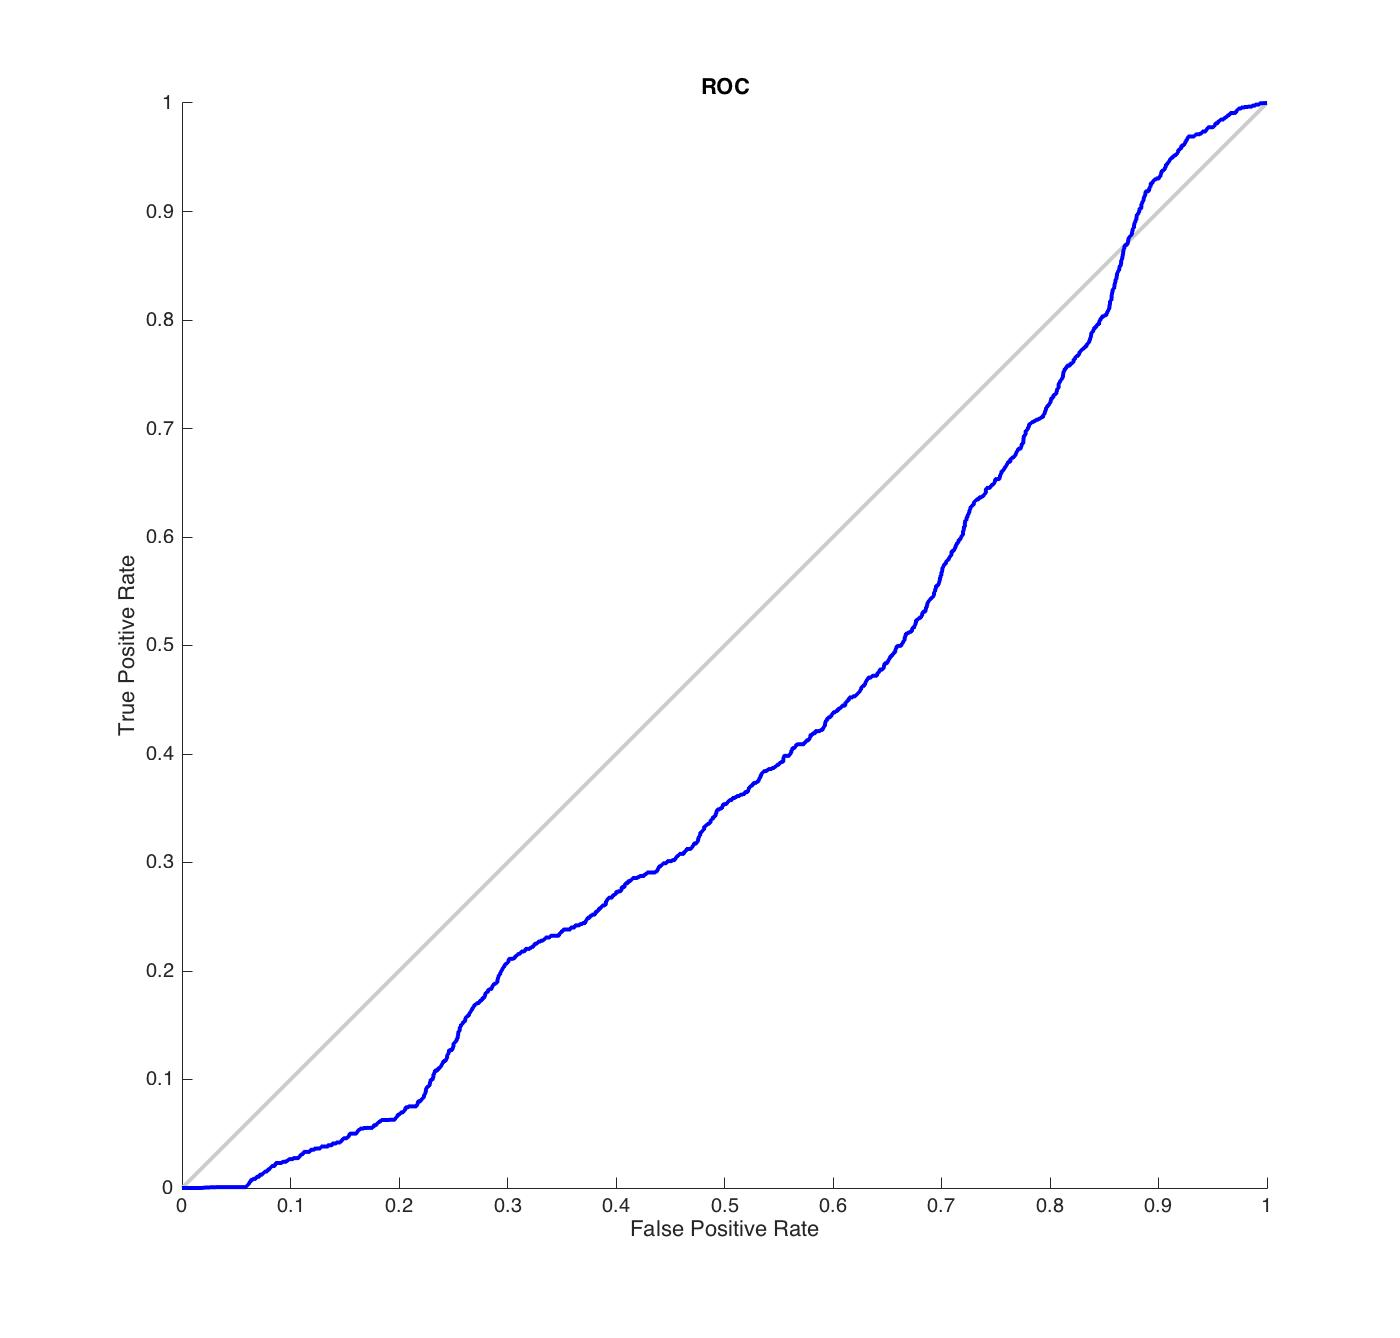
\includegraphics[width=\linewidth]{train_cc/roc_normal_global}
\endminipage\hfill
\minipage{0.53\textwidth}
  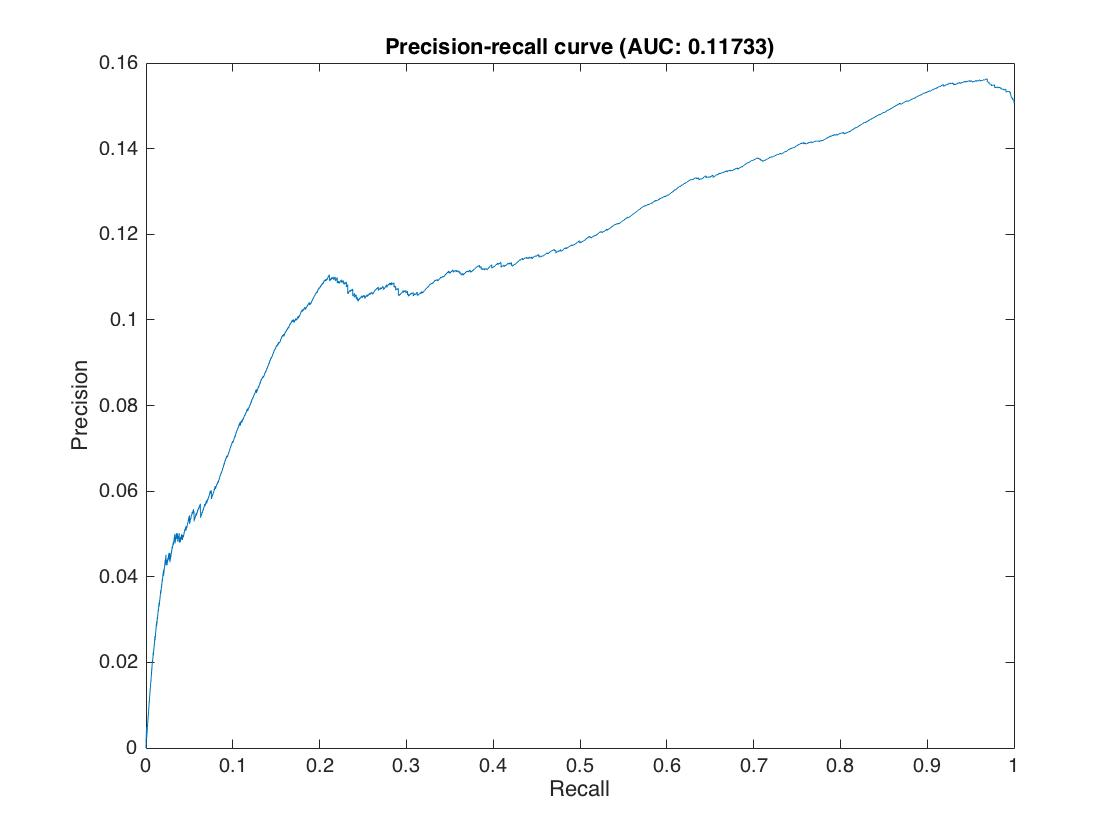
\includegraphics[width=\linewidth]{train_cc/prec_rec_normal_global}
\endminipage
\caption{ROC curve and Precision-Recall curve for classification without training, using the global reference value.}\label{fig:regiondetnormal}
\end{figure}

\subsubsection{Performance with SVM training over \emph{SplicedCC}}

\begin{figure}[!htb]
\minipage{0.42\textwidth}
  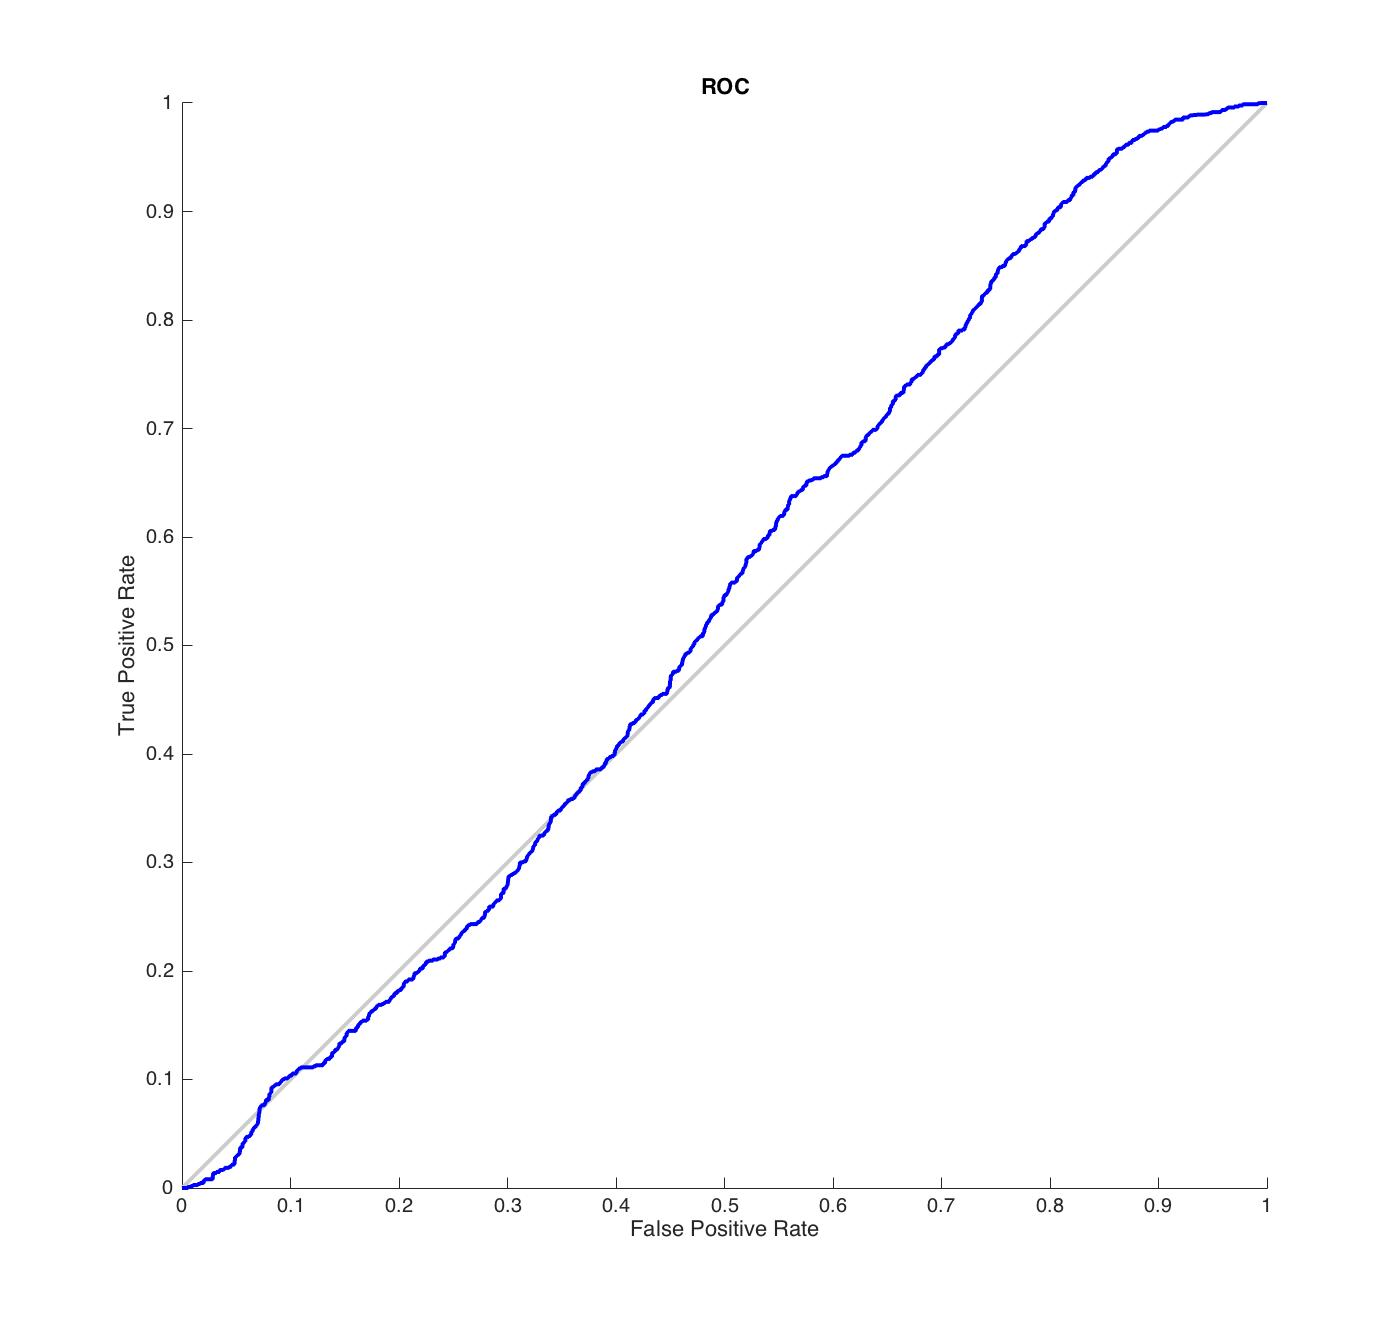
\includegraphics[width=\linewidth]{train_cc/roc_svm}
\endminipage\hfill
\minipage{0.53\textwidth}
  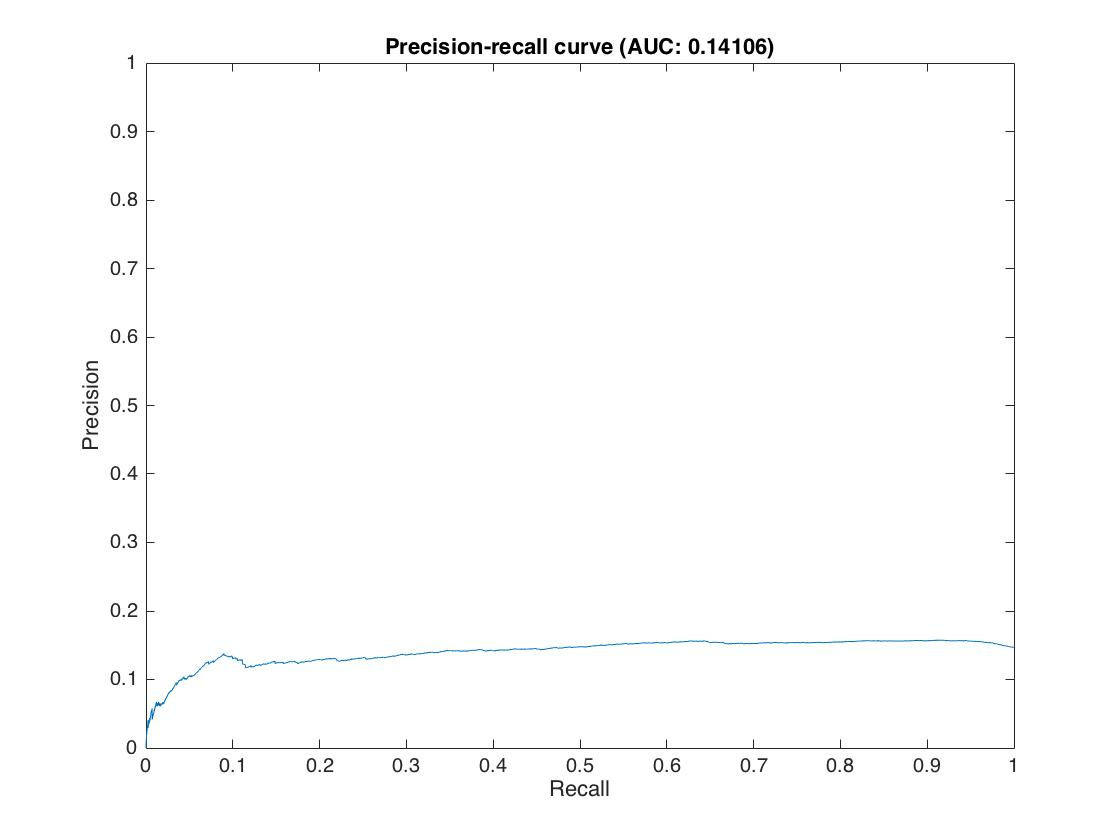
\includegraphics[width=\linewidth]{train_cc/prec_rec_svm}
\endminipage
\caption{ROC curve and Precision-Recall curve for classification with SVM training on \emph{SplicedCC}, using the global reference value.}\label{fig:regiondetnormal}
\end{figure}

\begin{figure}[!htb]
\minipage{0.42\textwidth}
  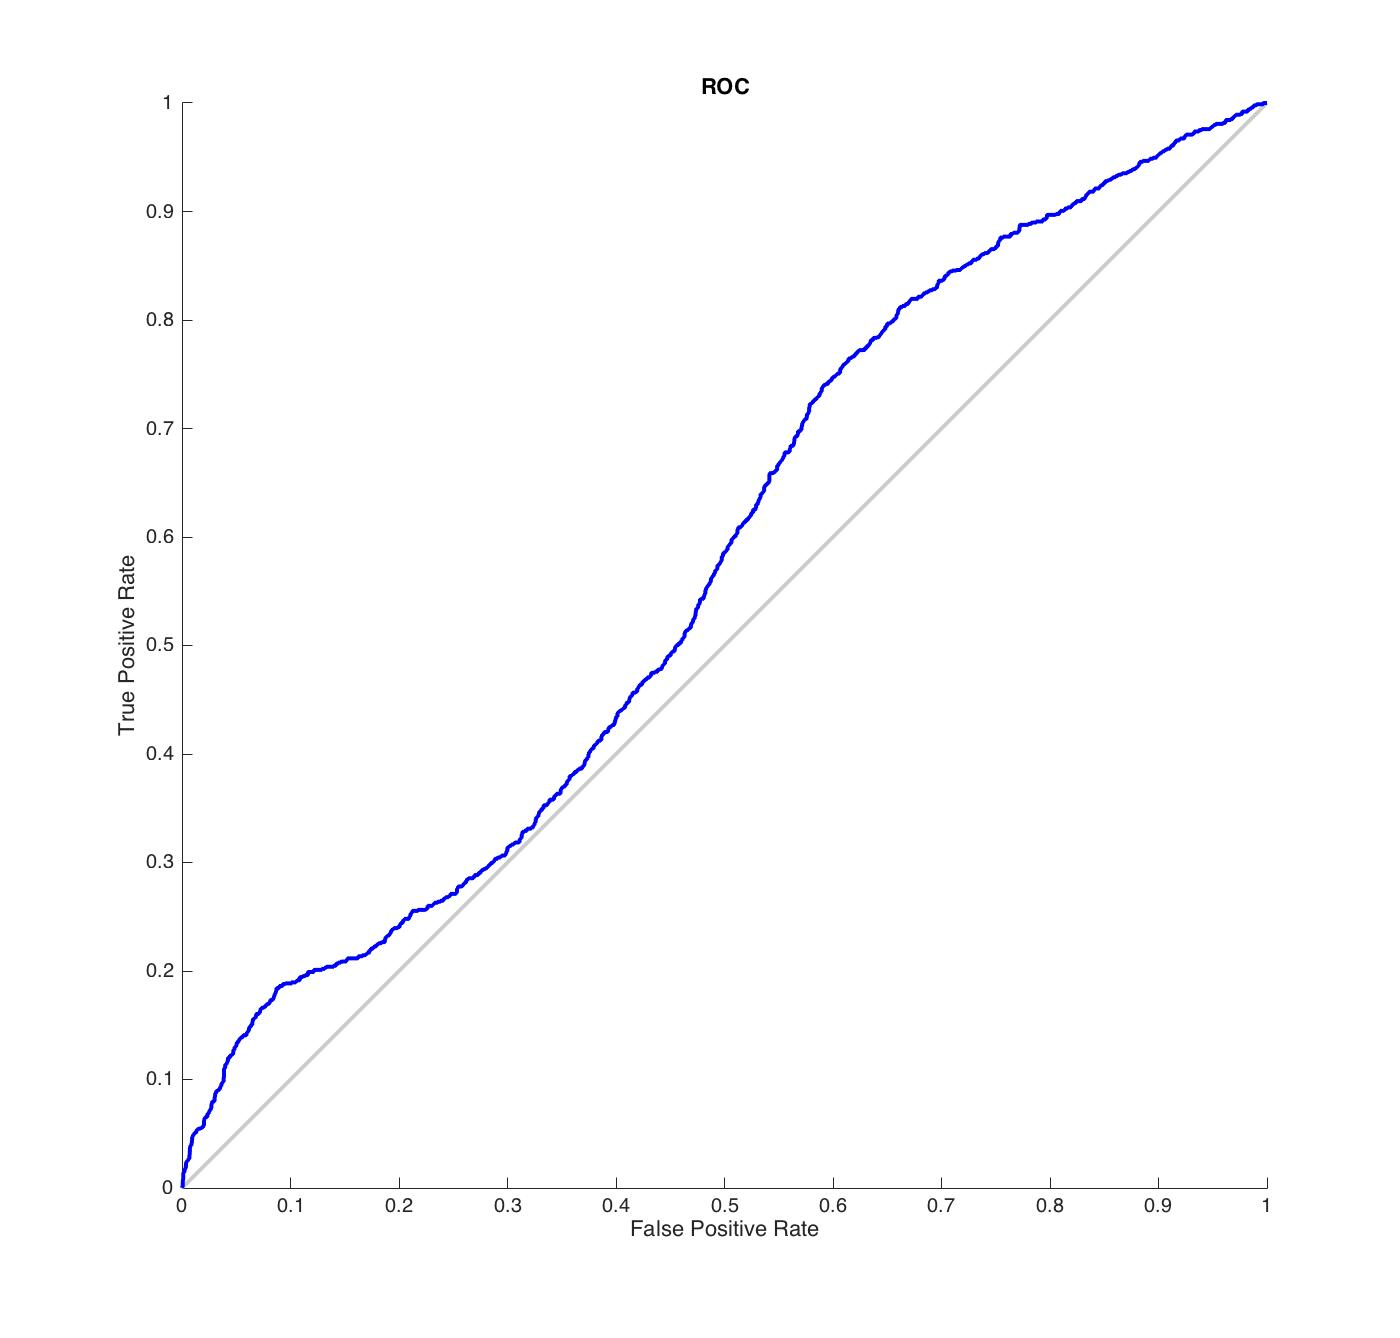
\includegraphics[width=\linewidth]{train_cc/roc_svm_global}
\endminipage\hfill
\minipage{0.53\textwidth}
  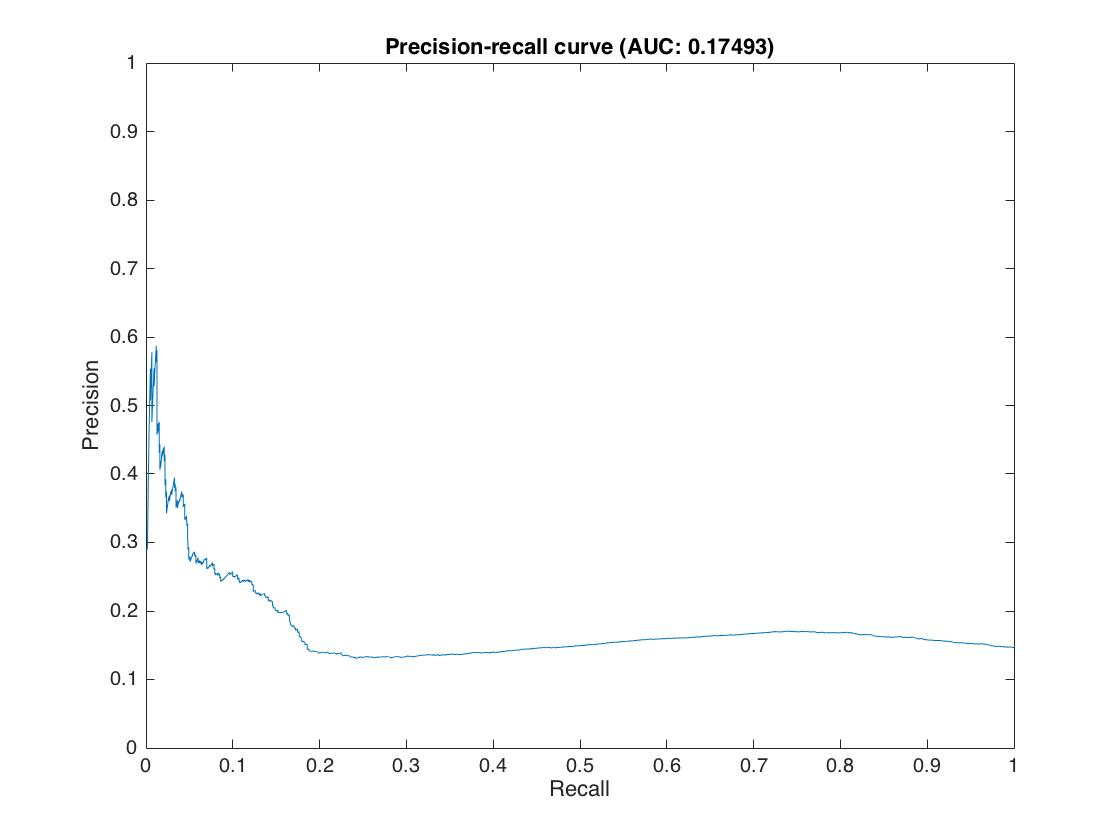
\includegraphics[width=\linewidth]{train_cc/prec_rec_svm_global}
\endminipage
\caption{ROC curve and Precision-Recall curve for classification with SVM training on \emph{SplicedCC}, using the global reference value.}\label{fig:regiondetnormal}
\end{figure}

\subsubsection{Performance with SVM training over \emph{SplicedDSO}}

\begin{figure}[!htb]
\minipage{0.42\textwidth}
  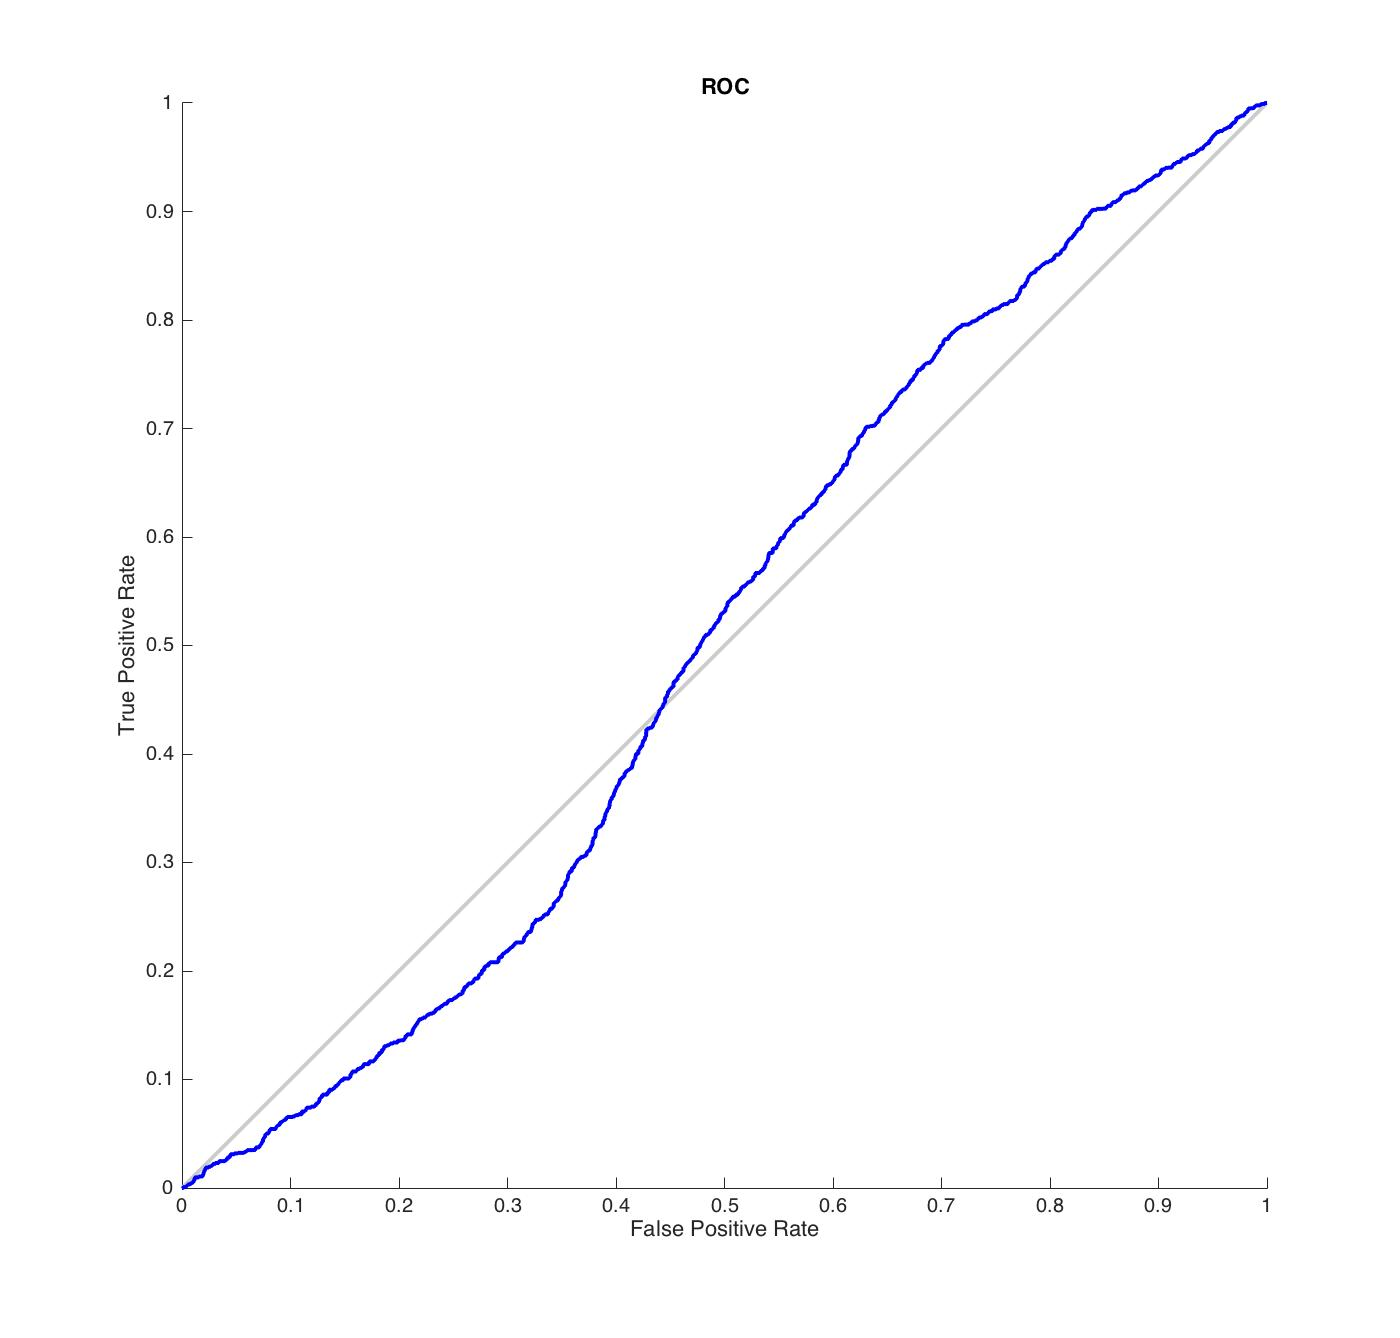
\includegraphics[width=\linewidth]{train_dso/roc_svm}
\endminipage\hfill
\minipage{0.53\textwidth}
  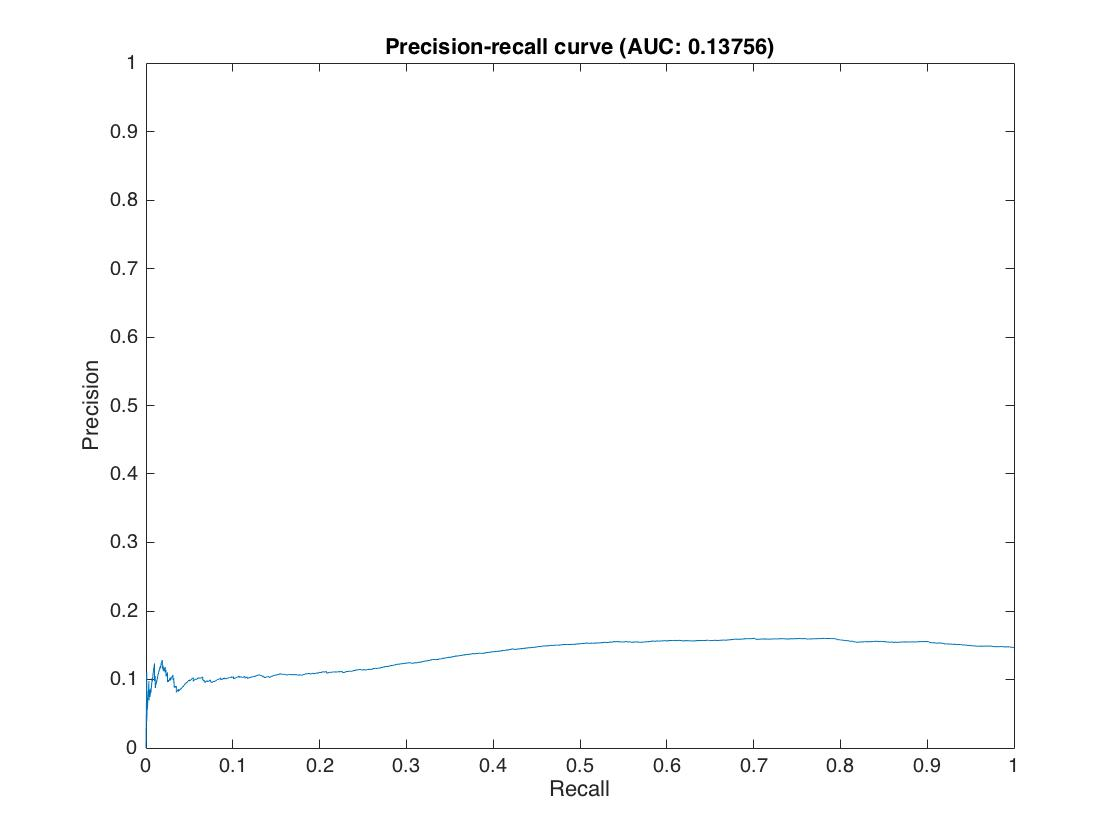
\includegraphics[width=\linewidth]{train_dso/prec_rec_svm}
\endminipage
\caption{ROC curve and Precision-Recall curve for classification with SVM training on \emph{SplicedDSO}, using the global reference value.}\label{fig:regiondetnormal}
\end{figure}

\begin{figure}[!htb]
\minipage{0.42\textwidth}
  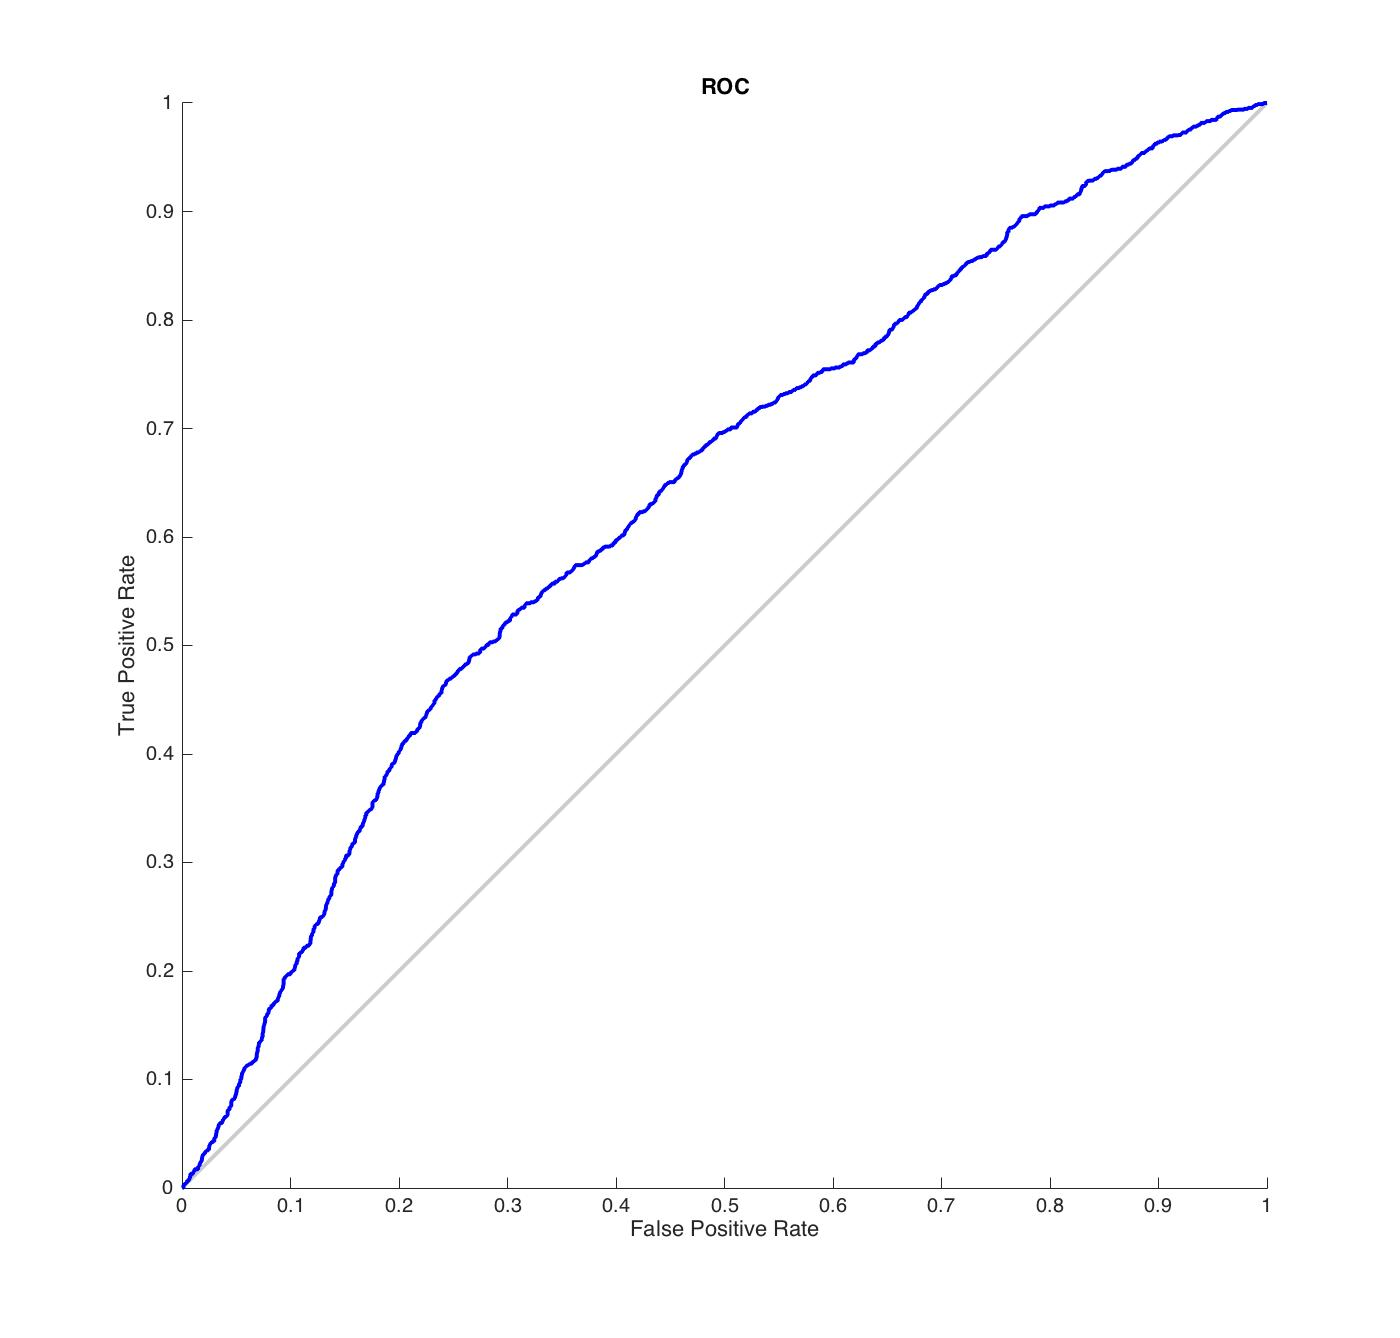
\includegraphics[width=\linewidth]{train_dso/roc_svm_global}
\endminipage\hfill
\minipage{0.53\textwidth}
  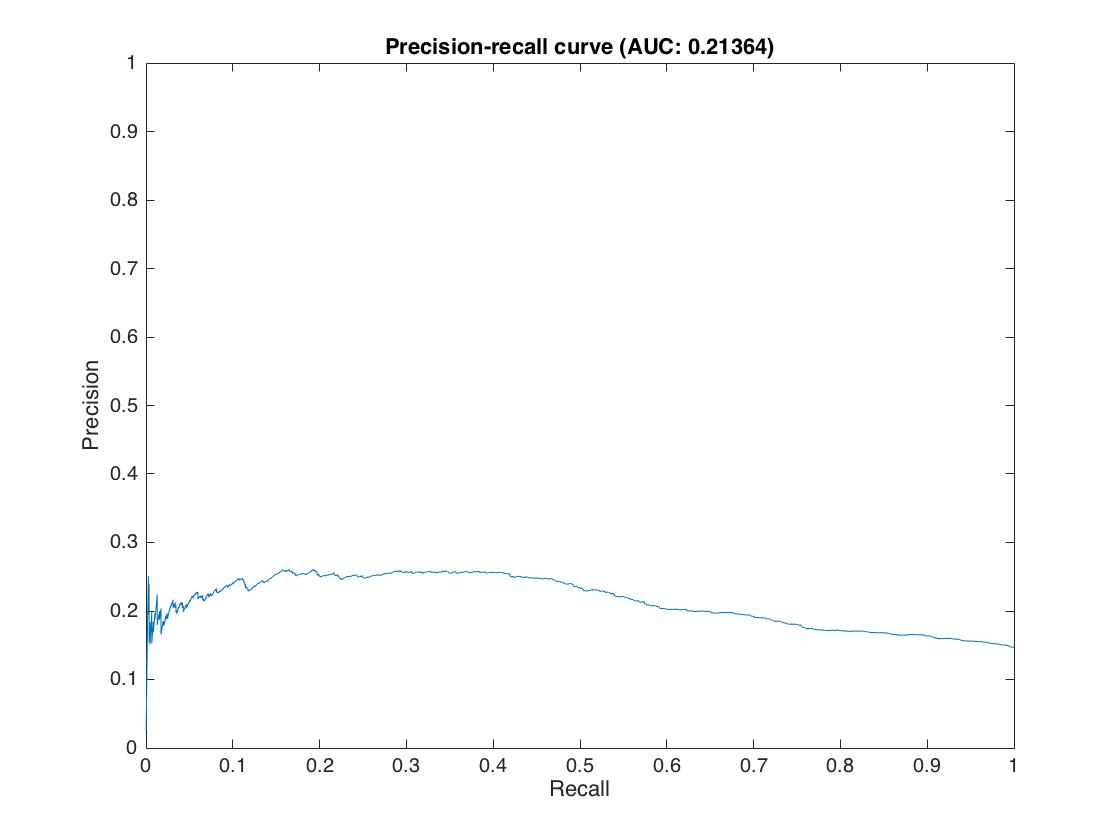
\includegraphics[width=\linewidth]{train_dso/prec_rec_svm_global}
\endminipage
\caption{ROC curve and Precision-Recall curve for classification with SVM training on \emph{SplicedDSO}, using the global reference value.}\label{fig:regiondetnormal}
\end{figure}


\chapter*{Conclusions}
\addcontentsline{toc}{chapter}{Conclusions}
\chaptermark{Conclusions}

Image composition is among the most common types of image manipulation and consists of using parts of two or more images to create a new fake one. In this context, this work has presented a method, composed by two different modules, that relies on illumination inconsistencies for detecting this image forgeries.

In the two different approaches, divided into two modules, proposed in Chapter 2, we analyzed illuminant maps entailing the interaction between the light source and the objects contained in a scene. The first module, aimed at detecting forgeries involving people, is based on the assumption that similar materials (\emph{e.g.} the human skin) illuminated by a common light source have similar properties in such maps.

As for research directions and future work, we suggest different contributions for each one of our proposed approaches. Future developments of this work may include the extension of the first module considering additional and different parts of body (\emph{e.g.}, all skin spots of the human body visible in an image). Given that our method compares skin material, it is feasible to use additional body parts, such as arms and legs, to increase the detection and confidence of the method.

Although promising as forensic evidence, methods that operate on illuminant color are inherently prone to estimation errors. Thus, we expect that further improvements can be achieved when more advanced illuminant color estimators become available.
}


\appendix
\chapter{Command line tool}

In this Appendix some implementation details are presented regarding the source code of the proposed approach. Source code of illuminant maps generation is available online\footnote{Christian Riess reasearch page for \emph{Scene Illumination as an Indicator of Image Manipulation} - https://www5.cs.fau.de/research/areas/computer-vision/image-forensics/scene-illumination-as-an-indicator-of-image-manipulation}.

The source code is divided into three parts:
\begin{itemize}
\item The two modules implemented separately (\emph{face-detector} and \emph{region-detector});
\item Illuminant maps estimation using IIC and GGE algorithms;
\item Image color descriptor extraction.
\end{itemize}

All code for the two main modules is written in Python using the open source computer vision library \emph{OpenCV}\footnote{OpenCV, Open Source Computer Vision Library -http://opencv.org}. OpenCV is an open source computer vision and machine learning software library built to provide a common infrastructure for computer vision applications. The library is written natively in C++, but it has C, Python, Java and MATLAB interfaces and supports Windows, Linux, Android and Mac OS.

Python version used is the \emph{3.4.2} and we used \emph{OpenCV 3.0.0}. 

The illuminant maps estimation algorithms implementation and image color descriptor codes are written in C++.

\begin{footnotesize}
\begin{verbatim}
ImageSplicingDetection v.0.5.1
usage: main.py 
            [-h] [--face-detector] [--region-detector] [--train] [--detect]
            [--evaluate] [--output-mask OUTPUT_MASK] [--display-result]
            [--crossvalidate] [--extract-single-features]
            [--no-extract-features] [--no-extract-maps] [--img IMG]
            [--euclidean-distances] [--heat-map] [--verbose]

optional arguments:
  -h, --help            show this help message and exit
  --face-detector       use face detector
  --region-detector     use region detector
  --train               train the model for further splicing detection
  --detect              detect splice over an image
  --evaluate            evaluate trained models over a set of images
  --output-mask OUTPUT_MASK
                        output mask path
  --display-result      display mask
  --crossvalidate       cross-validate the dataset
  --extract-single-features
                        extract feature vector for a specific image
  --no-extract-features
                        no extract all training images features
  --no-extract-maps     no extract all training images features
  --img IMG             the path of the suspicious image
  --euclidean-distances
                        visualize distances
  --heat-map            display the heat map between GGE and IIC maps
  --verbose             display all messages

\end{verbatim}
\end{footnotesize}


%%%  BACK MATTER  %%%  (bibliografia)
\backmatter

{
\bibliographystyle{ieee}
\bibliography{bibliography}
}

\chapter*{Ringraziamenti}
\addcontentsline{toc}{chapter}{Ringraziamenti}
\chaptermark{Ringraziamenti}

Per il percorso di tesi appena concluso vorrei innanzitutto ringraziare il Prof.~Alessandro Piva ed il Prof. Carlo Colombo per avermi dato la possibilità di poter contribuire a questo progetto. Un grande ringraziamento va poi al Dott.~Massimo Iuliani e al al Dott.~Marco Fanfani per tutto il tempo e il supporto a me dedicato durante tutto il lavoro svolto.

Un enorme grazie va a tutta la mia famiglia, a Samuele, Sonia e Sara, per avermi sempre sostenuto durante tutto il tempo dedicato allo studio ed aver creduto in me ogni giorno per tutti questi anni.

Un grazie va agli amici di sempre: Tommaso, Francesca, Lorenzo, Luca, Eleonora, Arianna, Claudia, Talita; il loro sostegno non è mai mancato, come non sono mai mancate le risate in compagnia.

Grazie ai miei compagni di corso e di studio, Tommaso e Saverio, che hanno contribuito a rendere più leggeri e piacevoli anche i momenti di studio più intenso.

Un grandissimo grazie va ad Agnese, per il suo supporto incodizionato, per la sua presenza anche nei momenti più difficili, per condividere e rendere sempre più speciale questo cammino.

Infine vorrei ringraziare tutti i presenti, anche quelli che possono esserlo solo con il pensiero, che sono o saranno con me a festeggiare questo giorno così speciale.
\end{document}

%pagina bianca (da usare, nei punti giusti, x avere una pag bianca invece che vuota con intestazione)
%\newpage{ \thispagestyle{empty}\null\vfil}